\documentclass[twoside]{book}

% Packages required by doxygen
\usepackage{fixltx2e}
\usepackage{calc}
\usepackage{doxygen}
\usepackage[export]{adjustbox} % also loads graphicx
\usepackage{graphicx}
\usepackage[utf8]{inputenc}
\usepackage{makeidx}
\usepackage{multicol}
\usepackage{multirow}
\PassOptionsToPackage{warn}{textcomp}
\usepackage{textcomp}
\usepackage[nointegrals]{wasysym}
\usepackage[table]{xcolor}

% Font selection
\usepackage[T1]{fontenc}
\usepackage[scaled=.90]{helvet}
\usepackage{courier}
\usepackage{amssymb}
\usepackage{sectsty}
\renewcommand{\familydefault}{\sfdefault}
\allsectionsfont{%
  \fontseries{bc}\selectfont%
  \color{darkgray}%
}
\renewcommand{\DoxyLabelFont}{%
  \fontseries{bc}\selectfont%
  \color{darkgray}%
}
\newcommand{\+}{\discretionary{\mbox{\scriptsize$\hookleftarrow$}}{}{}}

% Page & text layout
\usepackage{geometry}
\geometry{%
  a4paper,%
  top=2.5cm,%
  bottom=2.5cm,%
  left=2.5cm,%
  right=2.5cm%
}
\tolerance=750
\hfuzz=15pt
\hbadness=750
\setlength{\emergencystretch}{15pt}
\setlength{\parindent}{0cm}
\setlength{\parskip}{0.2cm}
\makeatletter
\renewcommand{\paragraph}{%
  \@startsection{paragraph}{4}{0ex}{-1.0ex}{1.0ex}{%
    \normalfont\normalsize\bfseries\SS@parafont%
  }%
}
\renewcommand{\subparagraph}{%
  \@startsection{subparagraph}{5}{0ex}{-1.0ex}{1.0ex}{%
    \normalfont\normalsize\bfseries\SS@subparafont%
  }%
}
\makeatother

% Headers & footers
\usepackage{fancyhdr}
\pagestyle{fancyplain}
\fancyhead[LE]{\fancyplain{}{\bfseries\thepage}}
\fancyhead[CE]{\fancyplain{}{}}
\fancyhead[RE]{\fancyplain{}{\bfseries\leftmark}}
\fancyhead[LO]{\fancyplain{}{\bfseries\rightmark}}
\fancyhead[CO]{\fancyplain{}{}}
\fancyhead[RO]{\fancyplain{}{\bfseries\thepage}}
\fancyfoot[LE]{\fancyplain{}{}}
\fancyfoot[CE]{\fancyplain{}{}}
\fancyfoot[RE]{\fancyplain{}{\bfseries\scriptsize Coroutine Manager Pro }}
\fancyfoot[LO]{\fancyplain{}{\bfseries\scriptsize Coroutine Manager Pro }}
\fancyfoot[CO]{\fancyplain{}{}}
\fancyfoot[RO]{\fancyplain{}{}}
\renewcommand{\footrulewidth}{0.4pt}
\renewcommand{\chaptermark}[1]{%
  \markboth{#1}{}%
}
\renewcommand{\sectionmark}[1]{%
  \markright{\thesection\ #1}%
}

% Indices & bibliography
\usepackage{natbib}
\usepackage[titles]{tocloft}
\setcounter{tocdepth}{3}
\setcounter{secnumdepth}{5}
\makeindex

% Hyperlinks (required, but should be loaded last)
\usepackage{ifpdf}
\ifpdf
  \usepackage[pdftex,pagebackref=true]{hyperref}
\else
  \usepackage[ps2pdf,pagebackref=true]{hyperref}
\fi
\hypersetup{%
  colorlinks=true,%
  linkcolor=blue,%
  citecolor=blue,%
  unicode%
}

% Custom commands
\newcommand{\clearemptydoublepage}{%
  \newpage{\pagestyle{empty}\cleardoublepage}%
}


%===== C O N T E N T S =====

\begin{document}

% Titlepage & ToC
\hypersetup{pageanchor=false,
             bookmarks=true,
             bookmarksnumbered=true,
             pdfencoding=unicode
            }
\pagenumbering{roman}
\begin{titlepage}
\vspace*{7cm}
\begin{center}%
{\Large Coroutine Manager Pro \\[1ex]\large 1.\+0 }\\
\vspace*{0.5cm}
{\small Mon Jan 4 2016 15:58:08}\\
\end{center}
\end{titlepage}
\clearemptydoublepage
\tableofcontents
\clearemptydoublepage
\pagenumbering{arabic}
\hypersetup{pageanchor=true}

%--- Begin generated contents ---
\chapter{Hierarchical Index}
\section{Class Hierarchy}
This inheritance list is sorted roughly, but not completely, alphabetically\+:\begin{DoxyCompactList}
\item \contentsline{section}{C\+M\+\_\+\+Global\+Coroutine\+Manager$<$ T $>$}{\pageref{class_c_m___global_coroutine_manager}}{}
\item \contentsline{section}{C\+M\+\_\+\+Global\+Coroutine\+Manager$<$ C\+M\+\_\+\+Job\+Manager $>$}{\pageref{class_c_m___global_coroutine_manager}}{}
\begin{DoxyCompactList}
\item \contentsline{section}{C\+M\+\_\+\+Job\+Manager}{\pageref{class_c_m___job_manager}}{}
\end{DoxyCompactList}
\item \contentsline{section}{C\+M\+\_\+\+Global\+Coroutine\+Manager$<$ C\+M\+\_\+\+Job\+Queue $>$}{\pageref{class_c_m___global_coroutine_manager}}{}
\begin{DoxyCompactList}
\item \contentsline{section}{C\+M\+\_\+\+Job\+Queue}{\pageref{class_c_m___job_queue}}{}
\end{DoxyCompactList}
\item \contentsline{section}{C\+M\+\_\+\+Singleton$<$ C\+M\+\_\+\+Dispatcher $>$}{\pageref{class_c_m___singleton}}{}
\begin{DoxyCompactList}
\item \contentsline{section}{C\+M\+\_\+\+Dispatcher}{\pageref{class_c_m___dispatcher}}{}
\end{DoxyCompactList}
\item \contentsline{section}{C\+M\+\_\+\+Singleton$<$ C\+M\+\_\+\+Logger $>$}{\pageref{class_c_m___singleton}}{}
\begin{DoxyCompactList}
\item \contentsline{section}{C\+M\+\_\+\+Logger}{\pageref{class_c_m___logger}}{}
\end{DoxyCompactList}
\item Event\+Args\begin{DoxyCompactList}
\item \contentsline{section}{C\+M\+\_\+\+Job\+Event\+Args}{\pageref{class_c_m___job_event_args}}{}
\item \contentsline{section}{C\+M\+\_\+\+Job\+Manager\+Event\+Args}{\pageref{class_c_m___job_manager_event_args}}{}
\item \contentsline{section}{C\+M\+\_\+\+Job\+Manager\+Job\+Edited\+Event\+Args}{\pageref{class_c_m___job_manager_job_edited_event_args}}{}
\item \contentsline{section}{C\+M\+\_\+\+Queue\+Event\+Args}{\pageref{class_c_m___queue_event_args}}{}
\end{DoxyCompactList}
\item \contentsline{section}{I\+C\+M\+\_\+\+Cloneable$<$ T $>$}{\pageref{interface_i_c_m___cloneable}}{}
\item \contentsline{section}{I\+C\+M\+\_\+\+Cloneable$<$ C\+M\+\_\+\+Job $>$}{\pageref{interface_i_c_m___cloneable}}{}
\begin{DoxyCompactList}
\item \contentsline{section}{C\+M\+\_\+\+Job}{\pageref{class_c_m___job}}{}
\end{DoxyCompactList}
\item \contentsline{section}{I\+C\+M\+\_\+\+Cloneable$<$ C\+M\+\_\+\+Job\+Queue $>$}{\pageref{interface_i_c_m___cloneable}}{}
\begin{DoxyCompactList}
\item \contentsline{section}{C\+M\+\_\+\+Job\+Queue}{\pageref{class_c_m___job_queue}}{}
\end{DoxyCompactList}
\item \contentsline{section}{C\+M\+\_\+\+Logger.\+Message}{\pageref{class_c_m___logger_1_1_message}}{}
\item Mono\+Behaviour\begin{DoxyCompactList}
\item \contentsline{section}{C\+M\+\_\+\+Singleton$<$ T $>$}{\pageref{class_c_m___singleton}}{}
\item \contentsline{section}{Example\+Character\+Damage}{\pageref{class_example_character_damage}}{}
\item \contentsline{section}{Example\+Character\+Movement}{\pageref{class_example_character_movement}}{}
\item \contentsline{section}{Example\+Continous\+Spawner}{\pageref{class_example_continous_spawner}}{}
\item \contentsline{section}{Example\+Damage\+Applier}{\pageref{class_example_damage_applier}}{}
\item \contentsline{section}{Example\+G\+U\+I}{\pageref{class_example_g_u_i}}{}
\item \contentsline{section}{Example\+Job\+Manager\+Test}{\pageref{class_example_job_manager_test}}{}
\item \contentsline{section}{Example\+Job\+Queue\+Test}{\pageref{class_example_job_queue_test}}{}
\item \contentsline{section}{Example\+Job\+Test}{\pageref{class_example_job_test}}{}
\item \contentsline{section}{Example\+Timer}{\pageref{class_example_timer}}{}
\item \contentsline{section}{Example\+T\+Imer\+Pause\+Resume}{\pageref{class_example_t_imer_pause_resume}}{}
\end{DoxyCompactList}
\end{DoxyCompactList}

\chapter{Class Index}
\section{Class List}
Here are the classes, structs, unions and interfaces with brief descriptions\+:\begin{DoxyCompactList}
\item\contentsline{section}{\hyperlink{class_c_m___dispatcher}{C\+M\+\_\+\+Dispatcher} \\*Used to start coroutines in the main thread from seperate threads. }{\pageref{class_c_m___dispatcher}}{}
\item\contentsline{section}{\hyperlink{class_c_m___global_coroutine_manager}{C\+M\+\_\+\+Global\+Coroutine\+Manager$<$ T $>$} \\*The base class of Global Coroutine Managers. Provides access to a singular global copy of the class. }{\pageref{class_c_m___global_coroutine_manager}}{}
\item\contentsline{section}{\hyperlink{class_c_m___job}{C\+M\+\_\+\+Job} \\*The main coroutine job class. Encapsulates the behaviour for a single coroutine job. Provides access to status (i.\+e. running, paused, killed etc), }{\pageref{class_c_m___job}}{}
\item\contentsline{section}{\hyperlink{class_c_m___job_event_args}{C\+M\+\_\+\+Job\+Event\+Args} \\*Arguements used in events raised by \hyperlink{class_c_m___job}{C\+M\+\_\+\+Job}. }{\pageref{class_c_m___job_event_args}}{}
\item\contentsline{section}{\hyperlink{class_c_m___job_manager}{C\+M\+\_\+\+Job\+Manager} \\*The main job manager class. Encapsulates the behaviour for global and local job managers. Provides access to events and public access to stored jobs. }{\pageref{class_c_m___job_manager}}{}
\item\contentsline{section}{\hyperlink{class_c_m___job_manager_event_args}{C\+M\+\_\+\+Job\+Manager\+Event\+Args} \\*Arguements used in events raised by \hyperlink{class_c_m___job_manager}{C\+M\+\_\+\+Job\+Manager}. }{\pageref{class_c_m___job_manager_event_args}}{}
\item\contentsline{section}{\hyperlink{class_c_m___job_manager_job_edited_event_args}{C\+M\+\_\+\+Job\+Manager\+Job\+Edited\+Event\+Args} \\*Arguements used in events raised by \hyperlink{class_c_m___job_manager}{C\+M\+\_\+\+Job\+Manager}. }{\pageref{class_c_m___job_manager_job_edited_event_args}}{}
\item\contentsline{section}{\hyperlink{class_c_m___job_queue}{C\+M\+\_\+\+Job\+Queue} \\*The main job queue class. Encapsulates all behaviour related to queueing a job. Provides access to events, and status (i.\+e. running, repeating). }{\pageref{class_c_m___job_queue}}{}
\item\contentsline{section}{\hyperlink{class_c_m___logger}{C\+M\+\_\+\+Logger} \\*Simple logging class used by the Coroutine Manager. }{\pageref{class_c_m___logger}}{}
\item\contentsline{section}{\hyperlink{class_c_m___queue_event_args}{C\+M\+\_\+\+Queue\+Event\+Args} \\*Arguements used by events raised by \hyperlink{class_c_m___job_queue}{C\+M\+\_\+\+Job\+Queue}. }{\pageref{class_c_m___queue_event_args}}{}
\item\contentsline{section}{\hyperlink{class_c_m___singleton}{C\+M\+\_\+\+Singleton$<$ T $>$} \\*A base class for any Singleton. Provides global singular access to a Mono\+Behaviour. }{\pageref{class_c_m___singleton}}{}
\item\contentsline{section}{\hyperlink{class_example_character_damage}{Example\+Character\+Damage} \\*Example character with action queue. }{\pageref{class_example_character_damage}}{}
\item\contentsline{section}{\hyperlink{class_example_character_movement}{Example\+Character\+Movement} \\*Example Script. A simple script showing how you can use \hyperlink{class_c_m___job_queue}{C\+M\+\_\+\+Job\+Queue} to create easily repeatable character movement. }{\pageref{class_example_character_movement}}{}
\item\contentsline{section}{\hyperlink{class_example_continous_spawner}{Example\+Continous\+Spawner} \\*Example Script. Used to spawn a number of objects using \hyperlink{class_c_m___job}{C\+M\+\_\+\+Job}. }{\pageref{class_example_continous_spawner}}{}
\item\contentsline{section}{\hyperlink{class_example_damage_applier}{Example\+Damage\+Applier} \\*Applies damage actions to the example character. }{\pageref{class_example_damage_applier}}{}
\item\contentsline{section}{\hyperlink{class_example_g_u_i}{Example\+G\+U\+I} \\*Simple G\+U\+I controller. Uses a \hyperlink{class_c_m___job_queue}{C\+M\+\_\+\+Job\+Queue} to enqueue a number of gui actions. }{\pageref{class_example_g_u_i}}{}
\item\contentsline{section}{\hyperlink{class_example_job_manager_test}{Example\+Job\+Manager\+Test} \\*Includes a number of methods to test the functionality of the \hyperlink{class_c_m___job_manager}{C\+M\+\_\+\+Job\+Manager} class. Each method showcases a particular functionality of the \hyperlink{class_c_m___job_manager}{C\+M\+\_\+\+Job\+Manager} that you can implement in your own projects. }{\pageref{class_example_job_manager_test}}{}
\item\contentsline{section}{\hyperlink{class_example_job_queue_test}{Example\+Job\+Queue\+Test} \\*Includes a number of methods to test the functionality of the \hyperlink{class_c_m___job_queue}{C\+M\+\_\+\+Job\+Queue} class. Each method showcases a particular functionality of the \hyperlink{class_c_m___job_queue}{C\+M\+\_\+\+Job\+Queue} that you can implement in your own projects. Each method returns an ienumerator so that it can added to a seperate job queue to be run in sequence for test purposes. }{\pageref{class_example_job_queue_test}}{}
\item\contentsline{section}{\hyperlink{class_example_job_test}{Example\+Job\+Test} \\*Includes a number of methods to test the functionality of the \hyperlink{class_c_m___job}{C\+M\+\_\+\+Job} class. Each method showcases a particular functionality of the \hyperlink{class_c_m___job}{C\+M\+\_\+\+Job} class that you can implement in your own projects. Each method returns an ienumerator so that it can added to a job queue to be run in sequence for test purposes. }{\pageref{class_example_job_test}}{}
\item\contentsline{section}{\hyperlink{class_example_timer}{Example\+Timer} \\*Creates new coroutine job to update a text object with time since startup. Adds job to global job manager so that it can be paused and resumed as required. }{\pageref{class_example_timer}}{}
\item\contentsline{section}{\hyperlink{class_example_t_imer_pause_resume}{Example\+T\+Imer\+Pause\+Resume} \\*Pauses all jobs associated with the Job\+Manager when user clicks left mouse button and resumes all jobs with user clicks right mouse button. }{\pageref{class_example_t_imer_pause_resume}}{}
\item\contentsline{section}{\hyperlink{interface_i_c_m___cloneable}{I\+C\+M\+\_\+\+Cloneable$<$ T $>$} \\*An interface for all classes used by the coroutine manager that can be cloned. }{\pageref{interface_i_c_m___cloneable}}{}
\item\contentsline{section}{\hyperlink{class_c_m___logger_1_1_message}{C\+M\+\_\+\+Logger.\+Message} \\*Encapsulates a message used by \hyperlink{class_c_m___logger}{C\+M\+\_\+\+Logger}. }{\pageref{class_c_m___logger_1_1_message}}{}
\end{DoxyCompactList}

\chapter{Class Documentation}
\hypertarget{class_c_m___dispatcher}{}\section{C\+M\+\_\+\+Dispatcher Class Reference}
\label{class_c_m___dispatcher}\index{C\+M\+\_\+\+Dispatcher@{C\+M\+\_\+\+Dispatcher}}


Used to start coroutines in the main thread from seperate threads.  


Inheritance diagram for C\+M\+\_\+\+Dispatcher\+:\begin{figure}[H]
\begin{center}
\leavevmode
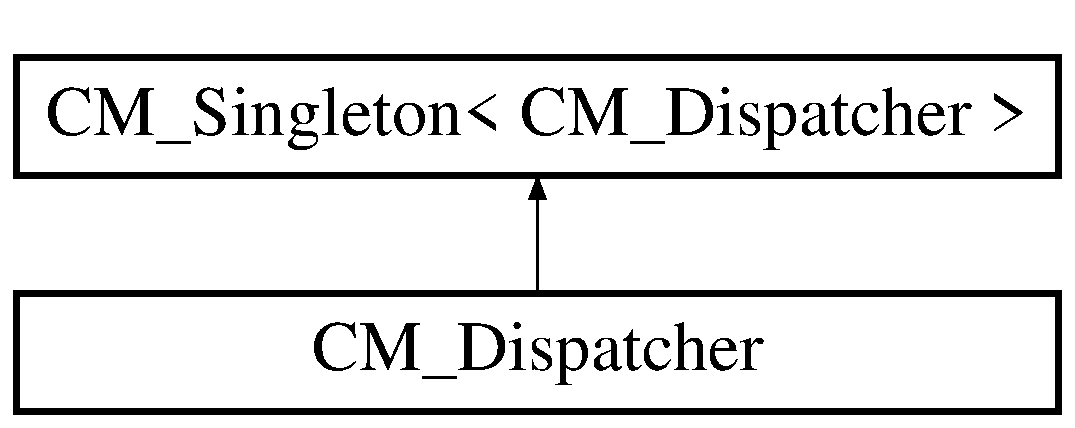
\includegraphics[height=2.000000cm]{class_c_m___dispatcher}
\end{center}
\end{figure}
\subsection*{Public Member Functions}
\begin{DoxyCompactItemize}
\item 
void \hyperlink{class_c_m___dispatcher_a1cdbca41b92b6d2d9bdca7c989c96b2a}{Add\+To\+Execute\+Queue} (I\+Enumerator job)
\begin{DoxyCompactList}\small\item\em Adds to execute queue. Coroutines in the queue are executed during the next timestep in the update method. \end{DoxyCompactList}\end{DoxyCompactItemize}
\subsection*{Additional Inherited Members}


\subsection{Detailed Description}
Used to start coroutines in the main thread from seperate threads. 



\subsection{Member Function Documentation}
\hypertarget{class_c_m___dispatcher_a1cdbca41b92b6d2d9bdca7c989c96b2a}{}\index{C\+M\+\_\+\+Dispatcher@{C\+M\+\_\+\+Dispatcher}!Add\+To\+Execute\+Queue@{Add\+To\+Execute\+Queue}}
\index{Add\+To\+Execute\+Queue@{Add\+To\+Execute\+Queue}!C\+M\+\_\+\+Dispatcher@{C\+M\+\_\+\+Dispatcher}}
\subsubsection[{Add\+To\+Execute\+Queue(\+I\+Enumerator job)}]{\setlength{\rightskip}{0pt plus 5cm}void C\+M\+\_\+\+Dispatcher.\+Add\+To\+Execute\+Queue (
\begin{DoxyParamCaption}
\item[{I\+Enumerator}]{job}
\end{DoxyParamCaption}
)}\label{class_c_m___dispatcher_a1cdbca41b92b6d2d9bdca7c989c96b2a}


Adds to execute queue. Coroutines in the queue are executed during the next timestep in the update method. 


\begin{DoxyParams}{Parameters}
{\em job} & Job.\\
\hline
\end{DoxyParams}


The documentation for this class was generated from the following file\+:\begin{DoxyCompactItemize}
\item 
C\+M\+\_\+\+Dispatcher.\+cs\end{DoxyCompactItemize}

\hypertarget{class_c_m___global_coroutine_manager}{}\section{C\+M\+\_\+\+Global\+Coroutine\+Manager$<$ T $>$ Class Template Reference}
\label{class_c_m___global_coroutine_manager}\index{C\+M\+\_\+\+Global\+Coroutine\+Manager$<$ T $>$@{C\+M\+\_\+\+Global\+Coroutine\+Manager$<$ T $>$}}


The base class of Global Coroutine Managers. Provides access to a singular global copy of the class.  


\subsection*{Protected Member Functions}
\begin{DoxyCompactItemize}
\item 
\hypertarget{class_c_m___global_coroutine_manager_a72523bcc2452962a1b1b5f8c4e6c6c12}{}virtual \hyperlink{class_c_m___job}{C\+M\+\_\+\+Job} {\bfseries Make\+Job} (string id, I\+Enumerator routine, bool add\+Listener\+To\+On\+Complete=true)\label{class_c_m___global_coroutine_manager_a72523bcc2452962a1b1b5f8c4e6c6c12}

\item 
\hypertarget{class_c_m___global_coroutine_manager_a2d14d4bf53d589e977a23b35443cbc77}{}virtual \hyperlink{class_c_m___job}{C\+M\+\_\+\+Job} {\bfseries Make\+Job} (\hyperlink{class_c_m___job}{C\+M\+\_\+\+Job} job)\label{class_c_m___global_coroutine_manager_a2d14d4bf53d589e977a23b35443cbc77}

\item 
\hypertarget{class_c_m___global_coroutine_manager_af0738a3e1dd19c1e8469ced62cc4d7aa}{}void {\bfseries Auto\+Generate\+Job\+Id} (\hyperlink{class_c_m___job}{C\+M\+\_\+\+Job} job)\label{class_c_m___global_coroutine_manager_af0738a3e1dd19c1e8469ced62cc4d7aa}

\item 
\hypertarget{class_c_m___global_coroutine_manager_a40fc4c4c48edf30f1c22d261f636463e}{}abstract void {\bfseries Handlejob\+Complete} (object sender, \hyperlink{class_c_m___job_event_args}{C\+M\+\_\+\+Job\+Event\+Args} e)\label{class_c_m___global_coroutine_manager_a40fc4c4c48edf30f1c22d261f636463e}

\end{DoxyCompactItemize}
\subsection*{Properties}
\begin{DoxyCompactItemize}
\item 
static T \hyperlink{class_c_m___global_coroutine_manager_ad6d1dbbb92d1de12b8e1018cf62d3a31}{Global}\hspace{0.3cm}{\ttfamily  \mbox{[}get\mbox{]}}
\begin{DoxyCompactList}\small\item\em Access to a global instance. \end{DoxyCompactList}\end{DoxyCompactItemize}


\subsection{Detailed Description}
The base class of Global Coroutine Managers. Provides access to a singular global copy of the class. 

\begin{Desc}
\item[Type Constraints]\begin{description}
\item[{\em T} : {\em new()}]\end{description}
\end{Desc}


\subsection{Property Documentation}
\hypertarget{class_c_m___global_coroutine_manager_ad6d1dbbb92d1de12b8e1018cf62d3a31}{}\index{C\+M\+\_\+\+Global\+Coroutine\+Manager@{C\+M\+\_\+\+Global\+Coroutine\+Manager}!Global@{Global}}
\index{Global@{Global}!C\+M\+\_\+\+Global\+Coroutine\+Manager@{C\+M\+\_\+\+Global\+Coroutine\+Manager}}
\subsubsection[{Global}]{\setlength{\rightskip}{0pt plus 5cm}T {\bf C\+M\+\_\+\+Global\+Coroutine\+Manager}$<$ T $>$.Global\hspace{0.3cm}{\ttfamily [static]}, {\ttfamily [get]}}\label{class_c_m___global_coroutine_manager_ad6d1dbbb92d1de12b8e1018cf62d3a31}


Access to a global instance. 



The documentation for this class was generated from the following file\+:\begin{DoxyCompactItemize}
\item 
C\+M\+\_\+\+Global\+Coroutine\+Manager.\+cs\end{DoxyCompactItemize}

\hypertarget{class_c_m___job}{}\section{C\+M\+\_\+\+Job Class Reference}
\label{class_c_m___job}\index{C\+M\+\_\+\+Job@{C\+M\+\_\+\+Job}}


The main coroutine job class. Encapsulates the behaviour for a single coroutine job. Provides access to status (i.\+e. running, paused, killed etc),  


Inheritance diagram for C\+M\+\_\+\+Job\+:\begin{figure}[H]
\begin{center}
\leavevmode
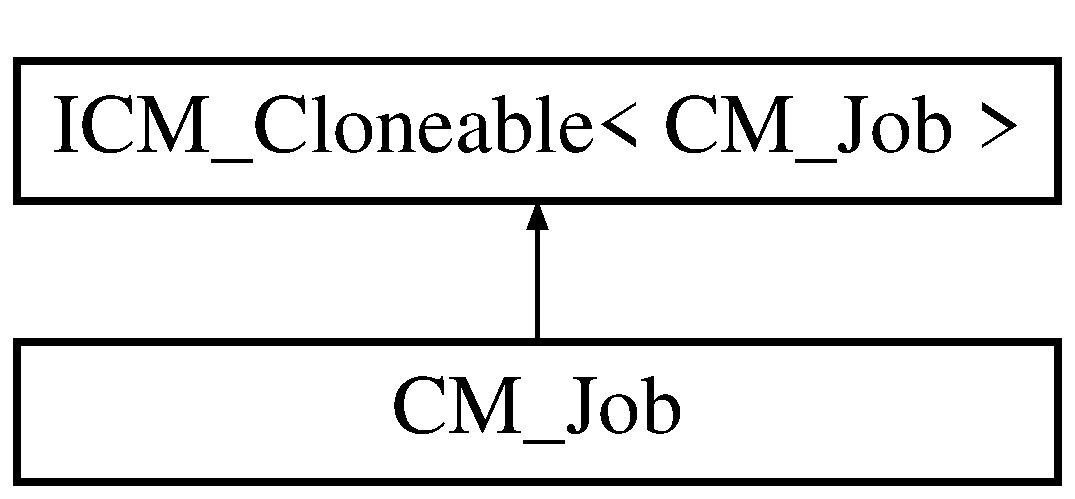
\includegraphics[height=2.000000cm]{class_c_m___job}
\end{center}
\end{figure}
\subsection*{Public Member Functions}
\begin{DoxyCompactItemize}
\item 
\hyperlink{class_c_m___job}{C\+M\+\_\+\+Job} \hyperlink{class_c_m___job_a7821bb2da3f3c9b30e171595a48aba7d}{Clone} ()
\begin{DoxyCompactList}\small\item\em Clone this instance. \end{DoxyCompactList}\item 
\hyperlink{class_c_m___job}{C\+M\+\_\+\+Job}\mbox{[}$\,$\mbox{]} \hyperlink{class_c_m___job_a1b1cd4972a357665fb21d20f58018b1e}{Clone} (int num\+Of\+Copies)
\begin{DoxyCompactList}\small\item\em Clone this instance. \end{DoxyCompactList}\item 
\hyperlink{class_c_m___job}{C\+M\+\_\+\+Job} \hyperlink{class_c_m___job_a54fd4dbd315708b9acd2a09f7096a554}{Start} ()
\begin{DoxyCompactList}\small\item\em Start this instance. Runs the coroutine immediately. \end{DoxyCompactList}\item 
\hyperlink{class_c_m___job}{C\+M\+\_\+\+Job} \hyperlink{class_c_m___job_a8c43918a2c837fe98cef1884da11836f}{Start} (float delay\+In\+Seconds)
\begin{DoxyCompactList}\small\item\em Start the specified instance after delay\+In\+Seconds. The coroutine is added to \hyperlink{class_c_m___dispatcher}{C\+M\+\_\+\+Dispatcher} job queue to be executed in the next timestep as a coroutine cannot be started in a seperate thread. \end{DoxyCompactList}\item 
\hyperlink{class_c_m___job}{C\+M\+\_\+\+Job} \hyperlink{class_c_m___job_a5b083485bb5892b17e180ff646a68a78}{Repeat} ()
\begin{DoxyCompactList}\small\item\em Sets this instance to repeat. The job is repeated when it has finished processing. \end{DoxyCompactList}\item 
\hyperlink{class_c_m___job}{C\+M\+\_\+\+Job} \hyperlink{class_c_m___job_a25e1a04eb72396ed2bf2b142d074d311}{Repeat} (int num\+Of\+Times)
\begin{DoxyCompactList}\small\item\em Sets this instance to repeat. The job is repeated a set number of times. \end{DoxyCompactList}\item 
\hypertarget{class_c_m___job_a3a7cfe0528790ce973e44c003a724459}{}\hyperlink{class_c_m___job}{C\+M\+\_\+\+Job} {\bfseries Stop\+Repeat} ()\label{class_c_m___job_a3a7cfe0528790ce973e44c003a724459}

\item 
\hyperlink{class_c_m___job}{C\+M\+\_\+\+Job} \hyperlink{class_c_m___job_a5ff8d362cc752f68ceed306837e36b8e}{Stop\+Repeat} (float delay\+In\+Seconds)
\begin{DoxyCompactList}\small\item\em Stops the repeat after a specified delay in seconds. \end{DoxyCompactList}\item 
\hyperlink{class_c_m___job}{C\+M\+\_\+\+Job} \hyperlink{class_c_m___job_aedbae0620e8da4cfc201f0dd3fc70c0e}{Pause} ()
\begin{DoxyCompactList}\small\item\em Pause this instance. \end{DoxyCompactList}\item 
\hyperlink{class_c_m___job}{C\+M\+\_\+\+Job} \hyperlink{class_c_m___job_a3cad9a52d6b2cbd773310f2d16943180}{Pause} (float delay\+In\+Seconds)
\begin{DoxyCompactList}\small\item\em Pause the specified instance after delay\+In\+Seconds. \end{DoxyCompactList}\item 
\hyperlink{class_c_m___job}{C\+M\+\_\+\+Job} \hyperlink{class_c_m___job_a17e7b235cb28ed51729f9235de1b576b}{Resume} ()
\begin{DoxyCompactList}\small\item\em Resume this instance. \end{DoxyCompactList}\item 
\hyperlink{class_c_m___job}{C\+M\+\_\+\+Job} \hyperlink{class_c_m___job_a5c68291f23790ca6be0941d4500ba3eb}{Resume} (float delay\+In\+Seconds)
\begin{DoxyCompactList}\small\item\em Resume the specified instance after delay\+In\+Seconds. \end{DoxyCompactList}\item 
void \hyperlink{class_c_m___job_a436839505339e2eb42c84de560a0874a}{Kill} ()
\begin{DoxyCompactList}\small\item\em Kill this instance. Stops the running coroutine. \end{DoxyCompactList}\item 
void \hyperlink{class_c_m___job_ac6413a58435cac4840e1dad8b53bd306}{Kill} (float delay\+In\+Seconds)
\begin{DoxyCompactList}\small\item\em Kill this instance. Stops the running coroutine after delay\+In\+Seconds. \end{DoxyCompactList}\item 
\hyperlink{class_c_m___job}{C\+M\+\_\+\+Job} \hyperlink{class_c_m___job_aa71a7f4fa664df6b7dd8f33f431f9935}{Add\+Child} (\hyperlink{class_c_m___job}{C\+M\+\_\+\+Job} child\+Job)
\begin{DoxyCompactList}\small\item\em Adds a child job. \end{DoxyCompactList}\item 
\hyperlink{class_c_m___job}{C\+M\+\_\+\+Job} \hyperlink{class_c_m___job_a9852216469080219798b397645d85767}{Add\+Child} (I\+Enumerator child\+Job)
\begin{DoxyCompactList}\small\item\em Create a new job using the provided Enumerator and adds as a child job. \end{DoxyCompactList}\item 
\hyperlink{class_c_m___job}{C\+M\+\_\+\+Job} \hyperlink{class_c_m___job_aaa110693cfb8ab6b8e35b7dafece2d32}{Remove\+Child\+Job} (\hyperlink{class_c_m___job}{C\+M\+\_\+\+Job} child\+Job)
\begin{DoxyCompactList}\small\item\em Removes a child job if present. \end{DoxyCompactList}\item 
\hyperlink{class_c_m___job}{C\+M\+\_\+\+Job} \hyperlink{class_c_m___job_a7b169aa2419e1b14bc5af2ef47bfbbe6}{Notify\+On\+Job\+Finished\+Running} (Event\+Handler$<$ \hyperlink{class_c_m___job_event_args}{C\+M\+\_\+\+Job\+Event\+Args} $>$ e)
\begin{DoxyCompactList}\small\item\em Subscribes to the job\+Finished\+Running event \end{DoxyCompactList}\item 
\hyperlink{class_c_m___job}{C\+M\+\_\+\+Job} \hyperlink{class_c_m___job_a0180557e1cfa03cf4a580f11711bb783}{Remove\+Notify\+On\+Job\+Finished\+Running} (Event\+Handler$<$ \hyperlink{class_c_m___job_event_args}{C\+M\+\_\+\+Job\+Event\+Args} $>$ e)
\begin{DoxyCompactList}\small\item\em Unsubscribes to the job\+Finished\+Running event \end{DoxyCompactList}\item 
\hyperlink{class_c_m___job}{C\+M\+\_\+\+Job} \hyperlink{class_c_m___job_a144f7f4f50fc9e78cb3cc89948b43781}{Notify\+On\+Job\+Started} (Event\+Handler$<$ \hyperlink{class_c_m___job_event_args}{C\+M\+\_\+\+Job\+Event\+Args} $>$ e)
\begin{DoxyCompactList}\small\item\em Subscribes to the job\+Started event. \end{DoxyCompactList}\item 
\hyperlink{class_c_m___job}{C\+M\+\_\+\+Job} \hyperlink{class_c_m___job_a136e32ada03eaab4c526b553d973f36f}{Remove\+Notify\+On\+Job\+Started} (Event\+Handler$<$ \hyperlink{class_c_m___job_event_args}{C\+M\+\_\+\+Job\+Event\+Args} $>$ e)
\begin{DoxyCompactList}\small\item\em Unsubscribes to the job\+Started event. \end{DoxyCompactList}\item 
\hyperlink{class_c_m___job}{C\+M\+\_\+\+Job} \hyperlink{class_c_m___job_a656895b36f0619ae50563993c25cd8c0}{Notify\+On\+Job\+Paused} (Event\+Handler$<$ \hyperlink{class_c_m___job_event_args}{C\+M\+\_\+\+Job\+Event\+Args} $>$ e)
\begin{DoxyCompactList}\small\item\em Subscribes to the job paused event. \end{DoxyCompactList}\item 
\hyperlink{class_c_m___job}{C\+M\+\_\+\+Job} \hyperlink{class_c_m___job_a1d12a9e9f851bb722e00c5982ff1fd08}{Remove\+Notify\+On\+Job\+Paused} (Event\+Handler$<$ \hyperlink{class_c_m___job_event_args}{C\+M\+\_\+\+Job\+Event\+Args} $>$ e)
\begin{DoxyCompactList}\small\item\em Unsubscribes to the job paused event. \end{DoxyCompactList}\item 
\hyperlink{class_c_m___job}{C\+M\+\_\+\+Job} \hyperlink{class_c_m___job_a75f17a64e339db10f3b8fb75fb240a0b}{Notify\+On\+Job\+Resumed} (Event\+Handler$<$ \hyperlink{class_c_m___job_event_args}{C\+M\+\_\+\+Job\+Event\+Args} $>$ e)
\begin{DoxyCompactList}\small\item\em Subscribes to the job resumed event. \end{DoxyCompactList}\item 
\hyperlink{class_c_m___job}{C\+M\+\_\+\+Job} \hyperlink{class_c_m___job_ab6821efdd6ee49603d1148b80483ef23}{Remove\+Notify\+On\+Job\+Resumed} (Event\+Handler$<$ \hyperlink{class_c_m___job_event_args}{C\+M\+\_\+\+Job\+Event\+Args} $>$ e)
\begin{DoxyCompactList}\small\item\em Unsubscribes to the job resumed event. \end{DoxyCompactList}\item 
\hyperlink{class_c_m___job}{C\+M\+\_\+\+Job} \hyperlink{class_c_m___job_aad8e48e0d2fa17fde30ba76516dbf7bd}{Notify\+On\+Job\+Complete} (Event\+Handler$<$ \hyperlink{class_c_m___job_event_args}{C\+M\+\_\+\+Job\+Event\+Args} $>$ e)
\begin{DoxyCompactList}\small\item\em Subscribes to the the job\+Complete event. \end{DoxyCompactList}\item 
\hyperlink{class_c_m___job}{C\+M\+\_\+\+Job} \hyperlink{class_c_m___job_a66b44002e5fcff452842af8750826453}{Remove\+Notify\+On\+Job\+Complete} (Event\+Handler$<$ \hyperlink{class_c_m___job_event_args}{C\+M\+\_\+\+Job\+Event\+Args} $>$ e)
\begin{DoxyCompactList}\small\item\em Unsubscribes to the the job\+Complete event. \end{DoxyCompactList}\item 
\hyperlink{class_c_m___job}{C\+M\+\_\+\+Job} \hyperlink{class_c_m___job_aadeb872e3ab5b90139e0d728f869be6c}{Notify\+On\+Child\+Job\+Started} (Event\+Handler$<$ \hyperlink{class_c_m___job_event_args}{C\+M\+\_\+\+Job\+Event\+Args} $>$ e)
\begin{DoxyCompactList}\small\item\em Subscribes to the the child\+Jobs\+Started event. \end{DoxyCompactList}\item 
\hyperlink{class_c_m___job}{C\+M\+\_\+\+Job} \hyperlink{class_c_m___job_aa1841d0fe84126d85c11a31c7b87c1ab}{Remove\+Notify\+On\+Child\+Job\+Started} (Event\+Handler$<$ \hyperlink{class_c_m___job_event_args}{C\+M\+\_\+\+Job\+Event\+Args} $>$ e)
\begin{DoxyCompactList}\small\item\em Unsubscribes to the the child\+Jobs\+Started event. \end{DoxyCompactList}\item 
\hyperlink{class_c_m___job}{C\+M\+\_\+\+Job} \hyperlink{class_c_m___job_aebb453c205c9817d621bea62f1716ae0}{Notify\+On\+Child\+Job\+Complete} (Event\+Handler$<$ \hyperlink{class_c_m___job_event_args}{C\+M\+\_\+\+Job\+Event\+Args} $>$ e)
\begin{DoxyCompactList}\small\item\em Subscribes to the the child\+Jobs\+Complete event. \end{DoxyCompactList}\item 
\hyperlink{class_c_m___job}{C\+M\+\_\+\+Job} \hyperlink{class_c_m___job_ac84b366bd233ee5970fd9f5841195d8b}{Remove\+Notify\+On\+Child\+Job\+Complete} (Event\+Handler$<$ \hyperlink{class_c_m___job_event_args}{C\+M\+\_\+\+Job\+Event\+Args} $>$ e)
\begin{DoxyCompactList}\small\item\em Unsubscribes to the the child\+Jobs\+Complete event. \end{DoxyCompactList}\end{DoxyCompactItemize}
\subsection*{Static Public Member Functions}
\begin{DoxyCompactItemize}
\item 
static \hyperlink{class_c_m___job}{C\+M\+\_\+\+Job} \hyperlink{class_c_m___job_a1ffab1654cb694e80dd1af68418048bb}{Make} (I\+Enumerator \hyperlink{class_c_m___job_a872a3e122dfc58a365f659918ba0fb82}{coroutine})
\begin{DoxyCompactList}\small\item\em Returns an initialised \hyperlink{class_c_m___job}{C\+M\+\_\+\+Job} instance. Provides static access to class. \end{DoxyCompactList}\item 
static \hyperlink{class_c_m___job}{C\+M\+\_\+\+Job} \hyperlink{class_c_m___job_ac2d0aa32b0e614d9a3133675c35a9866}{Make} (I\+Enumerator \hyperlink{class_c_m___job_a872a3e122dfc58a365f659918ba0fb82}{coroutine}, string \hyperlink{class_c_m___job_a19b93ec8fb1f643db06e79ad0710732b}{id})
\begin{DoxyCompactList}\small\item\em Returns an initialised \hyperlink{class_c_m___job}{C\+M\+\_\+\+Job} instance with the specified id. Provides static access to class. \end{DoxyCompactList}\item 
static \hyperlink{class_c_m___job}{C\+M\+\_\+\+Job}\mbox{[}$\,$\mbox{]} \hyperlink{class_c_m___job_a50cbb0f136c48addf0badefc62cecc6d}{Builder} (params I\+Enumerator\mbox{[}$\,$\mbox{]} coroutines)
\begin{DoxyCompactList}\small\item\em Builds the specified coroutines into \hyperlink{class_c_m___job}{C\+M\+\_\+\+Job} instances. \end{DoxyCompactList}\end{DoxyCompactItemize}
\subsection*{Protected Member Functions}
\begin{DoxyCompactItemize}
\item 
void \hyperlink{class_c_m___job_af33a79ea5b8e707fb79e594e580d4e17}{On\+Job\+Finished\+Running} (\hyperlink{class_c_m___job_event_args}{C\+M\+\_\+\+Job\+Event\+Args} e)
\begin{DoxyCompactList}\small\item\em Raises the job finished running event. \end{DoxyCompactList}\item 
void \hyperlink{class_c_m___job_a5b3aa9f1598fcf753be6fffad0f9a69a}{On\+Job\+Started} (\hyperlink{class_c_m___job_event_args}{C\+M\+\_\+\+Job\+Event\+Args} e)
\begin{DoxyCompactList}\small\item\em Raises the job started event. \end{DoxyCompactList}\item 
void \hyperlink{class_c_m___job_a6386d33b5ef65196a144598cb34fc12f}{On\+Job\+Complete} (\hyperlink{class_c_m___job_event_args}{C\+M\+\_\+\+Job\+Event\+Args} e)
\begin{DoxyCompactList}\small\item\em Raises the job complete event. \end{DoxyCompactList}\item 
void \hyperlink{class_c_m___job_a61f918b9776bf4437f3a0efa9cde64a2}{On\+Job\+Paused} (\hyperlink{class_c_m___job_event_args}{C\+M\+\_\+\+Job\+Event\+Args} e)
\begin{DoxyCompactList}\small\item\em Raises the job paused event. \end{DoxyCompactList}\item 
void \hyperlink{class_c_m___job_a6b6887d0dd433362ea571cdc4a419be1}{On\+Job\+Resumed} (\hyperlink{class_c_m___job_event_args}{C\+M\+\_\+\+Job\+Event\+Args} e)
\begin{DoxyCompactList}\small\item\em Raises the job resumed event. \end{DoxyCompactList}\item 
void \hyperlink{class_c_m___job_a39e81165ee12eb69e01e2052dd4add3e}{On\+Child\+Jobs\+Started} (\hyperlink{class_c_m___job_event_args}{C\+M\+\_\+\+Job\+Event\+Args} e)
\begin{DoxyCompactList}\small\item\em Raises the child jobs started event. \end{DoxyCompactList}\item 
void \hyperlink{class_c_m___job_a64f5a20ea7643b75584a1b63b8098011}{On\+Child\+Jobs\+Complete} (\hyperlink{class_c_m___job_event_args}{C\+M\+\_\+\+Job\+Event\+Args} e)
\begin{DoxyCompactList}\small\item\em Raises the child jobs complete event. \end{DoxyCompactList}\end{DoxyCompactItemize}
\subsection*{Properties}
\begin{DoxyCompactItemize}
\item 
string \hyperlink{class_c_m___job_a19b93ec8fb1f643db06e79ad0710732b}{id}\hspace{0.3cm}{\ttfamily  \mbox{[}get, set\mbox{]}}
\begin{DoxyCompactList}\small\item\em Gets or sets the identifier. The identifier is a unique key used by \hyperlink{class_c_m___job_manager}{C\+M\+\_\+\+Job\+Manager} to reference individual jobs. \end{DoxyCompactList}\item 
bool \hyperlink{class_c_m___job_a2226fbaee0c831d28fde43ffe0a58f70}{running}\hspace{0.3cm}{\ttfamily  \mbox{[}get\mbox{]}}
\begin{DoxyCompactList}\small\item\em Gets a value indicating whether this \hyperlink{class_c_m___job}{C\+M\+\_\+\+Job} is running. \end{DoxyCompactList}\item 
bool \hyperlink{class_c_m___job_a4d7d6001f3d1153d50f83490fe426925}{paused}\hspace{0.3cm}{\ttfamily  \mbox{[}get\mbox{]}}
\begin{DoxyCompactList}\small\item\em Gets a value indicating whether this \hyperlink{class_c_m___job}{C\+M\+\_\+\+Job} is paused. \end{DoxyCompactList}\item 
bool \hyperlink{class_c_m___job_aa15b9e9cead89bfbd449e0194dc30751}{job\+Killed}\hspace{0.3cm}{\ttfamily  \mbox{[}get\mbox{]}}
\begin{DoxyCompactList}\small\item\em Gets a value indicating whether this \hyperlink{class_c_m___job}{C\+M\+\_\+\+Job} job was killed or was allowed to complete. \end{DoxyCompactList}\item 
bool \hyperlink{class_c_m___job_ab18400e9cdb983c298d92c6e28acc599}{repeating}\hspace{0.3cm}{\ttfamily  \mbox{[}get\mbox{]}}
\begin{DoxyCompactList}\small\item\em Gets a value indicating whether this \hyperlink{class_c_m___job}{C\+M\+\_\+\+Job} is repeating. \end{DoxyCompactList}\item 
int \hyperlink{class_c_m___job_a042add3b81a210d7a98505bd53765ab5}{num\+Of\+Times\+Executed}\hspace{0.3cm}{\ttfamily  \mbox{[}get\mbox{]}}
\begin{DoxyCompactList}\small\item\em Gets the number of times this job has been executed. \end{DoxyCompactList}\item 
I\+Enumerator \hyperlink{class_c_m___job_a872a3e122dfc58a365f659918ba0fb82}{coroutine}\hspace{0.3cm}{\ttfamily  \mbox{[}get\mbox{]}}
\begin{DoxyCompactList}\small\item\em Gets the coroutine of this job. \end{DoxyCompactList}\end{DoxyCompactItemize}


\subsection{Detailed Description}
The main coroutine job class. Encapsulates the behaviour for a single coroutine job. Provides access to status (i.\+e. running, paused, killed etc), 



\subsection{Member Function Documentation}
\hypertarget{class_c_m___job_aa71a7f4fa664df6b7dd8f33f431f9935}{}\index{C\+M\+\_\+\+Job@{C\+M\+\_\+\+Job}!Add\+Child@{Add\+Child}}
\index{Add\+Child@{Add\+Child}!C\+M\+\_\+\+Job@{C\+M\+\_\+\+Job}}
\subsubsection[{Add\+Child(\+C\+M\+\_\+\+Job child\+Job)}]{\setlength{\rightskip}{0pt plus 5cm}{\bf C\+M\+\_\+\+Job} C\+M\+\_\+\+Job.\+Add\+Child (
\begin{DoxyParamCaption}
\item[{{\bf C\+M\+\_\+\+Job}}]{child\+Job}
\end{DoxyParamCaption}
)}\label{class_c_m___job_aa71a7f4fa664df6b7dd8f33f431f9935}


Adds a child job. 

\begin{DoxyReturn}{Returns}
The child.
\end{DoxyReturn}

\begin{DoxyParams}{Parameters}
{\em child\+Job} & Child job.\\
\hline
\end{DoxyParams}
\hypertarget{class_c_m___job_a9852216469080219798b397645d85767}{}\index{C\+M\+\_\+\+Job@{C\+M\+\_\+\+Job}!Add\+Child@{Add\+Child}}
\index{Add\+Child@{Add\+Child}!C\+M\+\_\+\+Job@{C\+M\+\_\+\+Job}}
\subsubsection[{Add\+Child(\+I\+Enumerator child\+Job)}]{\setlength{\rightskip}{0pt plus 5cm}{\bf C\+M\+\_\+\+Job} C\+M\+\_\+\+Job.\+Add\+Child (
\begin{DoxyParamCaption}
\item[{I\+Enumerator}]{child\+Job}
\end{DoxyParamCaption}
)}\label{class_c_m___job_a9852216469080219798b397645d85767}


Create a new job using the provided Enumerator and adds as a child job. 

\begin{DoxyReturn}{Returns}
The child.
\end{DoxyReturn}

\begin{DoxyParams}{Parameters}
{\em child\+Job} & Child job.\\
\hline
\end{DoxyParams}
\hypertarget{class_c_m___job_a50cbb0f136c48addf0badefc62cecc6d}{}\index{C\+M\+\_\+\+Job@{C\+M\+\_\+\+Job}!Builder@{Builder}}
\index{Builder@{Builder}!C\+M\+\_\+\+Job@{C\+M\+\_\+\+Job}}
\subsubsection[{Builder(params I\+Enumerator[] coroutines)}]{\setlength{\rightskip}{0pt plus 5cm}static {\bf C\+M\+\_\+\+Job} \mbox{[}$\,$\mbox{]} C\+M\+\_\+\+Job.\+Builder (
\begin{DoxyParamCaption}
\item[{params I\+Enumerator\mbox{[}$\,$\mbox{]}}]{coroutines}
\end{DoxyParamCaption}
)\hspace{0.3cm}{\ttfamily [static]}}\label{class_c_m___job_a50cbb0f136c48addf0badefc62cecc6d}


Builds the specified coroutines into \hyperlink{class_c_m___job}{C\+M\+\_\+\+Job} instances. 


\begin{DoxyParams}{Parameters}
{\em coroutines} & The built jobs.\\
\hline
\end{DoxyParams}
\hypertarget{class_c_m___job_a7821bb2da3f3c9b30e171595a48aba7d}{}\index{C\+M\+\_\+\+Job@{C\+M\+\_\+\+Job}!Clone@{Clone}}
\index{Clone@{Clone}!C\+M\+\_\+\+Job@{C\+M\+\_\+\+Job}}
\subsubsection[{Clone()}]{\setlength{\rightskip}{0pt plus 5cm}{\bf C\+M\+\_\+\+Job} C\+M\+\_\+\+Job.\+Clone (
\begin{DoxyParamCaption}
{}
\end{DoxyParamCaption}
)}\label{class_c_m___job_a7821bb2da3f3c9b30e171595a48aba7d}


Clone this instance. 

\hypertarget{class_c_m___job_a1b1cd4972a357665fb21d20f58018b1e}{}\index{C\+M\+\_\+\+Job@{C\+M\+\_\+\+Job}!Clone@{Clone}}
\index{Clone@{Clone}!C\+M\+\_\+\+Job@{C\+M\+\_\+\+Job}}
\subsubsection[{Clone(int num\+Of\+Copies)}]{\setlength{\rightskip}{0pt plus 5cm}{\bf C\+M\+\_\+\+Job} \mbox{[}$\,$\mbox{]} C\+M\+\_\+\+Job.\+Clone (
\begin{DoxyParamCaption}
\item[{int}]{num\+Of\+Copies}
\end{DoxyParamCaption}
)}\label{class_c_m___job_a1b1cd4972a357665fb21d20f58018b1e}


Clone this instance. 


\begin{DoxyParams}{Parameters}
{\em num\+Of\+Copies} & Number of copies to create.\\
\hline
\end{DoxyParams}
\hypertarget{class_c_m___job_a436839505339e2eb42c84de560a0874a}{}\index{C\+M\+\_\+\+Job@{C\+M\+\_\+\+Job}!Kill@{Kill}}
\index{Kill@{Kill}!C\+M\+\_\+\+Job@{C\+M\+\_\+\+Job}}
\subsubsection[{Kill()}]{\setlength{\rightskip}{0pt plus 5cm}void C\+M\+\_\+\+Job.\+Kill (
\begin{DoxyParamCaption}
{}
\end{DoxyParamCaption}
)}\label{class_c_m___job_a436839505339e2eb42c84de560a0874a}


Kill this instance. Stops the running coroutine. 

\hypertarget{class_c_m___job_ac6413a58435cac4840e1dad8b53bd306}{}\index{C\+M\+\_\+\+Job@{C\+M\+\_\+\+Job}!Kill@{Kill}}
\index{Kill@{Kill}!C\+M\+\_\+\+Job@{C\+M\+\_\+\+Job}}
\subsubsection[{Kill(float delay\+In\+Seconds)}]{\setlength{\rightskip}{0pt plus 5cm}void C\+M\+\_\+\+Job.\+Kill (
\begin{DoxyParamCaption}
\item[{float}]{delay\+In\+Seconds}
\end{DoxyParamCaption}
)}\label{class_c_m___job_ac6413a58435cac4840e1dad8b53bd306}


Kill this instance. Stops the running coroutine after delay\+In\+Seconds. 


\begin{DoxyParams}{Parameters}
{\em delay\+In\+Seconds} & Delay in seconds until instance killed.\\
\hline
\end{DoxyParams}
\hypertarget{class_c_m___job_a1ffab1654cb694e80dd1af68418048bb}{}\index{C\+M\+\_\+\+Job@{C\+M\+\_\+\+Job}!Make@{Make}}
\index{Make@{Make}!C\+M\+\_\+\+Job@{C\+M\+\_\+\+Job}}
\subsubsection[{Make(\+I\+Enumerator coroutine)}]{\setlength{\rightskip}{0pt plus 5cm}static {\bf C\+M\+\_\+\+Job} C\+M\+\_\+\+Job.\+Make (
\begin{DoxyParamCaption}
\item[{I\+Enumerator}]{coroutine}
\end{DoxyParamCaption}
)\hspace{0.3cm}{\ttfamily [static]}}\label{class_c_m___job_a1ffab1654cb694e80dd1af68418048bb}


Returns an initialised \hyperlink{class_c_m___job}{C\+M\+\_\+\+Job} instance. Provides static access to class. 


\begin{DoxyParams}{Parameters}
{\em coroutine} & Coroutine.\\
\hline
\end{DoxyParams}
\hypertarget{class_c_m___job_ac2d0aa32b0e614d9a3133675c35a9866}{}\index{C\+M\+\_\+\+Job@{C\+M\+\_\+\+Job}!Make@{Make}}
\index{Make@{Make}!C\+M\+\_\+\+Job@{C\+M\+\_\+\+Job}}
\subsubsection[{Make(\+I\+Enumerator coroutine, string id)}]{\setlength{\rightskip}{0pt plus 5cm}static {\bf C\+M\+\_\+\+Job} C\+M\+\_\+\+Job.\+Make (
\begin{DoxyParamCaption}
\item[{I\+Enumerator}]{coroutine, }
\item[{string}]{id}
\end{DoxyParamCaption}
)\hspace{0.3cm}{\ttfamily [static]}}\label{class_c_m___job_ac2d0aa32b0e614d9a3133675c35a9866}


Returns an initialised \hyperlink{class_c_m___job}{C\+M\+\_\+\+Job} instance with the specified id. Provides static access to class. 


\begin{DoxyParams}{Parameters}
{\em coroutine} & Coroutine.\\
\hline
{\em id} & Identifier.\\
\hline
\end{DoxyParams}
\hypertarget{class_c_m___job_aebb453c205c9817d621bea62f1716ae0}{}\index{C\+M\+\_\+\+Job@{C\+M\+\_\+\+Job}!Notify\+On\+Child\+Job\+Complete@{Notify\+On\+Child\+Job\+Complete}}
\index{Notify\+On\+Child\+Job\+Complete@{Notify\+On\+Child\+Job\+Complete}!C\+M\+\_\+\+Job@{C\+M\+\_\+\+Job}}
\subsubsection[{Notify\+On\+Child\+Job\+Complete(\+Event\+Handler$<$ C\+M\+\_\+\+Job\+Event\+Args $>$ e)}]{\setlength{\rightskip}{0pt plus 5cm}{\bf C\+M\+\_\+\+Job} C\+M\+\_\+\+Job.\+Notify\+On\+Child\+Job\+Complete (
\begin{DoxyParamCaption}
\item[{Event\+Handler$<$ {\bf C\+M\+\_\+\+Job\+Event\+Args} $>$}]{e}
\end{DoxyParamCaption}
)}\label{class_c_m___job_aebb453c205c9817d621bea62f1716ae0}


Subscribes to the the child\+Jobs\+Complete event. 


\begin{DoxyParams}{Parameters}
{\em e} & The eventhandler to be invoked on event.\\
\hline
\end{DoxyParams}
\hypertarget{class_c_m___job_aadeb872e3ab5b90139e0d728f869be6c}{}\index{C\+M\+\_\+\+Job@{C\+M\+\_\+\+Job}!Notify\+On\+Child\+Job\+Started@{Notify\+On\+Child\+Job\+Started}}
\index{Notify\+On\+Child\+Job\+Started@{Notify\+On\+Child\+Job\+Started}!C\+M\+\_\+\+Job@{C\+M\+\_\+\+Job}}
\subsubsection[{Notify\+On\+Child\+Job\+Started(\+Event\+Handler$<$ C\+M\+\_\+\+Job\+Event\+Args $>$ e)}]{\setlength{\rightskip}{0pt plus 5cm}{\bf C\+M\+\_\+\+Job} C\+M\+\_\+\+Job.\+Notify\+On\+Child\+Job\+Started (
\begin{DoxyParamCaption}
\item[{Event\+Handler$<$ {\bf C\+M\+\_\+\+Job\+Event\+Args} $>$}]{e}
\end{DoxyParamCaption}
)}\label{class_c_m___job_aadeb872e3ab5b90139e0d728f869be6c}


Subscribes to the the child\+Jobs\+Started event. 


\begin{DoxyParams}{Parameters}
{\em e} & The eventhandler to be invoked on event.\\
\hline
\end{DoxyParams}
\hypertarget{class_c_m___job_aad8e48e0d2fa17fde30ba76516dbf7bd}{}\index{C\+M\+\_\+\+Job@{C\+M\+\_\+\+Job}!Notify\+On\+Job\+Complete@{Notify\+On\+Job\+Complete}}
\index{Notify\+On\+Job\+Complete@{Notify\+On\+Job\+Complete}!C\+M\+\_\+\+Job@{C\+M\+\_\+\+Job}}
\subsubsection[{Notify\+On\+Job\+Complete(\+Event\+Handler$<$ C\+M\+\_\+\+Job\+Event\+Args $>$ e)}]{\setlength{\rightskip}{0pt plus 5cm}{\bf C\+M\+\_\+\+Job} C\+M\+\_\+\+Job.\+Notify\+On\+Job\+Complete (
\begin{DoxyParamCaption}
\item[{Event\+Handler$<$ {\bf C\+M\+\_\+\+Job\+Event\+Args} $>$}]{e}
\end{DoxyParamCaption}
)}\label{class_c_m___job_aad8e48e0d2fa17fde30ba76516dbf7bd}


Subscribes to the the job\+Complete event. 


\begin{DoxyParams}{Parameters}
{\em e} & The eventhandler to be invoked on event.\\
\hline
\end{DoxyParams}
\hypertarget{class_c_m___job_a7b169aa2419e1b14bc5af2ef47bfbbe6}{}\index{C\+M\+\_\+\+Job@{C\+M\+\_\+\+Job}!Notify\+On\+Job\+Finished\+Running@{Notify\+On\+Job\+Finished\+Running}}
\index{Notify\+On\+Job\+Finished\+Running@{Notify\+On\+Job\+Finished\+Running}!C\+M\+\_\+\+Job@{C\+M\+\_\+\+Job}}
\subsubsection[{Notify\+On\+Job\+Finished\+Running(\+Event\+Handler$<$ C\+M\+\_\+\+Job\+Event\+Args $>$ e)}]{\setlength{\rightskip}{0pt plus 5cm}{\bf C\+M\+\_\+\+Job} C\+M\+\_\+\+Job.\+Notify\+On\+Job\+Finished\+Running (
\begin{DoxyParamCaption}
\item[{Event\+Handler$<$ {\bf C\+M\+\_\+\+Job\+Event\+Args} $>$}]{e}
\end{DoxyParamCaption}
)}\label{class_c_m___job_a7b169aa2419e1b14bc5af2ef47bfbbe6}


Subscribes to the job\+Finished\+Running event 


\begin{DoxyParams}{Parameters}
{\em e} & The eventhandler to be invoked on event.\\
\hline
\end{DoxyParams}
\hypertarget{class_c_m___job_a656895b36f0619ae50563993c25cd8c0}{}\index{C\+M\+\_\+\+Job@{C\+M\+\_\+\+Job}!Notify\+On\+Job\+Paused@{Notify\+On\+Job\+Paused}}
\index{Notify\+On\+Job\+Paused@{Notify\+On\+Job\+Paused}!C\+M\+\_\+\+Job@{C\+M\+\_\+\+Job}}
\subsubsection[{Notify\+On\+Job\+Paused(\+Event\+Handler$<$ C\+M\+\_\+\+Job\+Event\+Args $>$ e)}]{\setlength{\rightskip}{0pt plus 5cm}{\bf C\+M\+\_\+\+Job} C\+M\+\_\+\+Job.\+Notify\+On\+Job\+Paused (
\begin{DoxyParamCaption}
\item[{Event\+Handler$<$ {\bf C\+M\+\_\+\+Job\+Event\+Args} $>$}]{e}
\end{DoxyParamCaption}
)}\label{class_c_m___job_a656895b36f0619ae50563993c25cd8c0}


Subscribes to the job paused event. 

\begin{DoxyReturn}{Returns}
The on job paused.
\end{DoxyReturn}

\begin{DoxyParams}{Parameters}
{\em e} & E.\\
\hline
\end{DoxyParams}
\hypertarget{class_c_m___job_a75f17a64e339db10f3b8fb75fb240a0b}{}\index{C\+M\+\_\+\+Job@{C\+M\+\_\+\+Job}!Notify\+On\+Job\+Resumed@{Notify\+On\+Job\+Resumed}}
\index{Notify\+On\+Job\+Resumed@{Notify\+On\+Job\+Resumed}!C\+M\+\_\+\+Job@{C\+M\+\_\+\+Job}}
\subsubsection[{Notify\+On\+Job\+Resumed(\+Event\+Handler$<$ C\+M\+\_\+\+Job\+Event\+Args $>$ e)}]{\setlength{\rightskip}{0pt plus 5cm}{\bf C\+M\+\_\+\+Job} C\+M\+\_\+\+Job.\+Notify\+On\+Job\+Resumed (
\begin{DoxyParamCaption}
\item[{Event\+Handler$<$ {\bf C\+M\+\_\+\+Job\+Event\+Args} $>$}]{e}
\end{DoxyParamCaption}
)}\label{class_c_m___job_a75f17a64e339db10f3b8fb75fb240a0b}


Subscribes to the job resumed event. 

\begin{DoxyReturn}{Returns}
The on job paused.
\end{DoxyReturn}

\begin{DoxyParams}{Parameters}
{\em e} & E.\\
\hline
\end{DoxyParams}
\hypertarget{class_c_m___job_a144f7f4f50fc9e78cb3cc89948b43781}{}\index{C\+M\+\_\+\+Job@{C\+M\+\_\+\+Job}!Notify\+On\+Job\+Started@{Notify\+On\+Job\+Started}}
\index{Notify\+On\+Job\+Started@{Notify\+On\+Job\+Started}!C\+M\+\_\+\+Job@{C\+M\+\_\+\+Job}}
\subsubsection[{Notify\+On\+Job\+Started(\+Event\+Handler$<$ C\+M\+\_\+\+Job\+Event\+Args $>$ e)}]{\setlength{\rightskip}{0pt plus 5cm}{\bf C\+M\+\_\+\+Job} C\+M\+\_\+\+Job.\+Notify\+On\+Job\+Started (
\begin{DoxyParamCaption}
\item[{Event\+Handler$<$ {\bf C\+M\+\_\+\+Job\+Event\+Args} $>$}]{e}
\end{DoxyParamCaption}
)}\label{class_c_m___job_a144f7f4f50fc9e78cb3cc89948b43781}


Subscribes to the job\+Started event. 


\begin{DoxyParams}{Parameters}
{\em e} & The eventhandler to be invoked on event.\\
\hline
\end{DoxyParams}
\hypertarget{class_c_m___job_a64f5a20ea7643b75584a1b63b8098011}{}\index{C\+M\+\_\+\+Job@{C\+M\+\_\+\+Job}!On\+Child\+Jobs\+Complete@{On\+Child\+Jobs\+Complete}}
\index{On\+Child\+Jobs\+Complete@{On\+Child\+Jobs\+Complete}!C\+M\+\_\+\+Job@{C\+M\+\_\+\+Job}}
\subsubsection[{On\+Child\+Jobs\+Complete(\+C\+M\+\_\+\+Job\+Event\+Args e)}]{\setlength{\rightskip}{0pt plus 5cm}void C\+M\+\_\+\+Job.\+On\+Child\+Jobs\+Complete (
\begin{DoxyParamCaption}
\item[{{\bf C\+M\+\_\+\+Job\+Event\+Args}}]{e}
\end{DoxyParamCaption}
)\hspace{0.3cm}{\ttfamily [protected]}}\label{class_c_m___job_a64f5a20ea7643b75584a1b63b8098011}


Raises the child jobs complete event. 


\begin{DoxyParams}{Parameters}
{\em e} & E.\\
\hline
\end{DoxyParams}
\hypertarget{class_c_m___job_a39e81165ee12eb69e01e2052dd4add3e}{}\index{C\+M\+\_\+\+Job@{C\+M\+\_\+\+Job}!On\+Child\+Jobs\+Started@{On\+Child\+Jobs\+Started}}
\index{On\+Child\+Jobs\+Started@{On\+Child\+Jobs\+Started}!C\+M\+\_\+\+Job@{C\+M\+\_\+\+Job}}
\subsubsection[{On\+Child\+Jobs\+Started(\+C\+M\+\_\+\+Job\+Event\+Args e)}]{\setlength{\rightskip}{0pt plus 5cm}void C\+M\+\_\+\+Job.\+On\+Child\+Jobs\+Started (
\begin{DoxyParamCaption}
\item[{{\bf C\+M\+\_\+\+Job\+Event\+Args}}]{e}
\end{DoxyParamCaption}
)\hspace{0.3cm}{\ttfamily [protected]}}\label{class_c_m___job_a39e81165ee12eb69e01e2052dd4add3e}


Raises the child jobs started event. 


\begin{DoxyParams}{Parameters}
{\em e} & E.\\
\hline
\end{DoxyParams}
\hypertarget{class_c_m___job_a6386d33b5ef65196a144598cb34fc12f}{}\index{C\+M\+\_\+\+Job@{C\+M\+\_\+\+Job}!On\+Job\+Complete@{On\+Job\+Complete}}
\index{On\+Job\+Complete@{On\+Job\+Complete}!C\+M\+\_\+\+Job@{C\+M\+\_\+\+Job}}
\subsubsection[{On\+Job\+Complete(\+C\+M\+\_\+\+Job\+Event\+Args e)}]{\setlength{\rightskip}{0pt plus 5cm}void C\+M\+\_\+\+Job.\+On\+Job\+Complete (
\begin{DoxyParamCaption}
\item[{{\bf C\+M\+\_\+\+Job\+Event\+Args}}]{e}
\end{DoxyParamCaption}
)\hspace{0.3cm}{\ttfamily [protected]}}\label{class_c_m___job_a6386d33b5ef65196a144598cb34fc12f}


Raises the job complete event. 


\begin{DoxyParams}{Parameters}
{\em e} & E.\\
\hline
\end{DoxyParams}
\hypertarget{class_c_m___job_af33a79ea5b8e707fb79e594e580d4e17}{}\index{C\+M\+\_\+\+Job@{C\+M\+\_\+\+Job}!On\+Job\+Finished\+Running@{On\+Job\+Finished\+Running}}
\index{On\+Job\+Finished\+Running@{On\+Job\+Finished\+Running}!C\+M\+\_\+\+Job@{C\+M\+\_\+\+Job}}
\subsubsection[{On\+Job\+Finished\+Running(\+C\+M\+\_\+\+Job\+Event\+Args e)}]{\setlength{\rightskip}{0pt plus 5cm}void C\+M\+\_\+\+Job.\+On\+Job\+Finished\+Running (
\begin{DoxyParamCaption}
\item[{{\bf C\+M\+\_\+\+Job\+Event\+Args}}]{e}
\end{DoxyParamCaption}
)\hspace{0.3cm}{\ttfamily [protected]}}\label{class_c_m___job_af33a79ea5b8e707fb79e594e580d4e17}


Raises the job finished running event. 


\begin{DoxyParams}{Parameters}
{\em e} & E.\\
\hline
\end{DoxyParams}
\hypertarget{class_c_m___job_a61f918b9776bf4437f3a0efa9cde64a2}{}\index{C\+M\+\_\+\+Job@{C\+M\+\_\+\+Job}!On\+Job\+Paused@{On\+Job\+Paused}}
\index{On\+Job\+Paused@{On\+Job\+Paused}!C\+M\+\_\+\+Job@{C\+M\+\_\+\+Job}}
\subsubsection[{On\+Job\+Paused(\+C\+M\+\_\+\+Job\+Event\+Args e)}]{\setlength{\rightskip}{0pt plus 5cm}void C\+M\+\_\+\+Job.\+On\+Job\+Paused (
\begin{DoxyParamCaption}
\item[{{\bf C\+M\+\_\+\+Job\+Event\+Args}}]{e}
\end{DoxyParamCaption}
)\hspace{0.3cm}{\ttfamily [protected]}}\label{class_c_m___job_a61f918b9776bf4437f3a0efa9cde64a2}


Raises the job paused event. 


\begin{DoxyParams}{Parameters}
{\em e} & E.\\
\hline
\end{DoxyParams}
\hypertarget{class_c_m___job_a6b6887d0dd433362ea571cdc4a419be1}{}\index{C\+M\+\_\+\+Job@{C\+M\+\_\+\+Job}!On\+Job\+Resumed@{On\+Job\+Resumed}}
\index{On\+Job\+Resumed@{On\+Job\+Resumed}!C\+M\+\_\+\+Job@{C\+M\+\_\+\+Job}}
\subsubsection[{On\+Job\+Resumed(\+C\+M\+\_\+\+Job\+Event\+Args e)}]{\setlength{\rightskip}{0pt plus 5cm}void C\+M\+\_\+\+Job.\+On\+Job\+Resumed (
\begin{DoxyParamCaption}
\item[{{\bf C\+M\+\_\+\+Job\+Event\+Args}}]{e}
\end{DoxyParamCaption}
)\hspace{0.3cm}{\ttfamily [protected]}}\label{class_c_m___job_a6b6887d0dd433362ea571cdc4a419be1}


Raises the job resumed event. 


\begin{DoxyParams}{Parameters}
{\em e} & E.\\
\hline
\end{DoxyParams}
\hypertarget{class_c_m___job_a5b3aa9f1598fcf753be6fffad0f9a69a}{}\index{C\+M\+\_\+\+Job@{C\+M\+\_\+\+Job}!On\+Job\+Started@{On\+Job\+Started}}
\index{On\+Job\+Started@{On\+Job\+Started}!C\+M\+\_\+\+Job@{C\+M\+\_\+\+Job}}
\subsubsection[{On\+Job\+Started(\+C\+M\+\_\+\+Job\+Event\+Args e)}]{\setlength{\rightskip}{0pt plus 5cm}void C\+M\+\_\+\+Job.\+On\+Job\+Started (
\begin{DoxyParamCaption}
\item[{{\bf C\+M\+\_\+\+Job\+Event\+Args}}]{e}
\end{DoxyParamCaption}
)\hspace{0.3cm}{\ttfamily [protected]}}\label{class_c_m___job_a5b3aa9f1598fcf753be6fffad0f9a69a}


Raises the job started event. 


\begin{DoxyParams}{Parameters}
{\em e} & E.\\
\hline
\end{DoxyParams}
\hypertarget{class_c_m___job_aedbae0620e8da4cfc201f0dd3fc70c0e}{}\index{C\+M\+\_\+\+Job@{C\+M\+\_\+\+Job}!Pause@{Pause}}
\index{Pause@{Pause}!C\+M\+\_\+\+Job@{C\+M\+\_\+\+Job}}
\subsubsection[{Pause()}]{\setlength{\rightskip}{0pt plus 5cm}{\bf C\+M\+\_\+\+Job} C\+M\+\_\+\+Job.\+Pause (
\begin{DoxyParamCaption}
{}
\end{DoxyParamCaption}
)}\label{class_c_m___job_aedbae0620e8da4cfc201f0dd3fc70c0e}


Pause this instance. 

\hypertarget{class_c_m___job_a3cad9a52d6b2cbd773310f2d16943180}{}\index{C\+M\+\_\+\+Job@{C\+M\+\_\+\+Job}!Pause@{Pause}}
\index{Pause@{Pause}!C\+M\+\_\+\+Job@{C\+M\+\_\+\+Job}}
\subsubsection[{Pause(float delay\+In\+Seconds)}]{\setlength{\rightskip}{0pt plus 5cm}{\bf C\+M\+\_\+\+Job} C\+M\+\_\+\+Job.\+Pause (
\begin{DoxyParamCaption}
\item[{float}]{delay\+In\+Seconds}
\end{DoxyParamCaption}
)}\label{class_c_m___job_a3cad9a52d6b2cbd773310f2d16943180}


Pause the specified instance after delay\+In\+Seconds. 


\begin{DoxyParams}{Parameters}
{\em delay\+In\+Secods} & Delay in secods until instance is paused.\\
\hline
\end{DoxyParams}
\hypertarget{class_c_m___job_aaa110693cfb8ab6b8e35b7dafece2d32}{}\index{C\+M\+\_\+\+Job@{C\+M\+\_\+\+Job}!Remove\+Child\+Job@{Remove\+Child\+Job}}
\index{Remove\+Child\+Job@{Remove\+Child\+Job}!C\+M\+\_\+\+Job@{C\+M\+\_\+\+Job}}
\subsubsection[{Remove\+Child\+Job(\+C\+M\+\_\+\+Job child\+Job)}]{\setlength{\rightskip}{0pt plus 5cm}{\bf C\+M\+\_\+\+Job} C\+M\+\_\+\+Job.\+Remove\+Child\+Job (
\begin{DoxyParamCaption}
\item[{{\bf C\+M\+\_\+\+Job}}]{child\+Job}
\end{DoxyParamCaption}
)}\label{class_c_m___job_aaa110693cfb8ab6b8e35b7dafece2d32}


Removes a child job if present. 

\begin{DoxyReturn}{Returns}
The child job.
\end{DoxyReturn}

\begin{DoxyParams}{Parameters}
{\em child\+Job} & Child job.\\
\hline
\end{DoxyParams}
\hypertarget{class_c_m___job_ac84b366bd233ee5970fd9f5841195d8b}{}\index{C\+M\+\_\+\+Job@{C\+M\+\_\+\+Job}!Remove\+Notify\+On\+Child\+Job\+Complete@{Remove\+Notify\+On\+Child\+Job\+Complete}}
\index{Remove\+Notify\+On\+Child\+Job\+Complete@{Remove\+Notify\+On\+Child\+Job\+Complete}!C\+M\+\_\+\+Job@{C\+M\+\_\+\+Job}}
\subsubsection[{Remove\+Notify\+On\+Child\+Job\+Complete(\+Event\+Handler$<$ C\+M\+\_\+\+Job\+Event\+Args $>$ e)}]{\setlength{\rightskip}{0pt plus 5cm}{\bf C\+M\+\_\+\+Job} C\+M\+\_\+\+Job.\+Remove\+Notify\+On\+Child\+Job\+Complete (
\begin{DoxyParamCaption}
\item[{Event\+Handler$<$ {\bf C\+M\+\_\+\+Job\+Event\+Args} $>$}]{e}
\end{DoxyParamCaption}
)}\label{class_c_m___job_ac84b366bd233ee5970fd9f5841195d8b}


Unsubscribes to the the child\+Jobs\+Complete event. 


\begin{DoxyParams}{Parameters}
{\em e} & The eventhandler to be unsubscribed.\\
\hline
\end{DoxyParams}
\hypertarget{class_c_m___job_aa1841d0fe84126d85c11a31c7b87c1ab}{}\index{C\+M\+\_\+\+Job@{C\+M\+\_\+\+Job}!Remove\+Notify\+On\+Child\+Job\+Started@{Remove\+Notify\+On\+Child\+Job\+Started}}
\index{Remove\+Notify\+On\+Child\+Job\+Started@{Remove\+Notify\+On\+Child\+Job\+Started}!C\+M\+\_\+\+Job@{C\+M\+\_\+\+Job}}
\subsubsection[{Remove\+Notify\+On\+Child\+Job\+Started(\+Event\+Handler$<$ C\+M\+\_\+\+Job\+Event\+Args $>$ e)}]{\setlength{\rightskip}{0pt plus 5cm}{\bf C\+M\+\_\+\+Job} C\+M\+\_\+\+Job.\+Remove\+Notify\+On\+Child\+Job\+Started (
\begin{DoxyParamCaption}
\item[{Event\+Handler$<$ {\bf C\+M\+\_\+\+Job\+Event\+Args} $>$}]{e}
\end{DoxyParamCaption}
)}\label{class_c_m___job_aa1841d0fe84126d85c11a31c7b87c1ab}


Unsubscribes to the the child\+Jobs\+Started event. 


\begin{DoxyParams}{Parameters}
{\em e} & The eventhandler to be unsubscribed.\\
\hline
\end{DoxyParams}
\hypertarget{class_c_m___job_a66b44002e5fcff452842af8750826453}{}\index{C\+M\+\_\+\+Job@{C\+M\+\_\+\+Job}!Remove\+Notify\+On\+Job\+Complete@{Remove\+Notify\+On\+Job\+Complete}}
\index{Remove\+Notify\+On\+Job\+Complete@{Remove\+Notify\+On\+Job\+Complete}!C\+M\+\_\+\+Job@{C\+M\+\_\+\+Job}}
\subsubsection[{Remove\+Notify\+On\+Job\+Complete(\+Event\+Handler$<$ C\+M\+\_\+\+Job\+Event\+Args $>$ e)}]{\setlength{\rightskip}{0pt plus 5cm}{\bf C\+M\+\_\+\+Job} C\+M\+\_\+\+Job.\+Remove\+Notify\+On\+Job\+Complete (
\begin{DoxyParamCaption}
\item[{Event\+Handler$<$ {\bf C\+M\+\_\+\+Job\+Event\+Args} $>$}]{e}
\end{DoxyParamCaption}
)}\label{class_c_m___job_a66b44002e5fcff452842af8750826453}


Unsubscribes to the the job\+Complete event. 


\begin{DoxyParams}{Parameters}
{\em e} & The eventhandler to be unsubscribed.\\
\hline
\end{DoxyParams}
\hypertarget{class_c_m___job_a0180557e1cfa03cf4a580f11711bb783}{}\index{C\+M\+\_\+\+Job@{C\+M\+\_\+\+Job}!Remove\+Notify\+On\+Job\+Finished\+Running@{Remove\+Notify\+On\+Job\+Finished\+Running}}
\index{Remove\+Notify\+On\+Job\+Finished\+Running@{Remove\+Notify\+On\+Job\+Finished\+Running}!C\+M\+\_\+\+Job@{C\+M\+\_\+\+Job}}
\subsubsection[{Remove\+Notify\+On\+Job\+Finished\+Running(\+Event\+Handler$<$ C\+M\+\_\+\+Job\+Event\+Args $>$ e)}]{\setlength{\rightskip}{0pt plus 5cm}{\bf C\+M\+\_\+\+Job} C\+M\+\_\+\+Job.\+Remove\+Notify\+On\+Job\+Finished\+Running (
\begin{DoxyParamCaption}
\item[{Event\+Handler$<$ {\bf C\+M\+\_\+\+Job\+Event\+Args} $>$}]{e}
\end{DoxyParamCaption}
)}\label{class_c_m___job_a0180557e1cfa03cf4a580f11711bb783}


Unsubscribes to the job\+Finished\+Running event 


\begin{DoxyParams}{Parameters}
{\em e} & The eventhandler to be invoked on event.\\
\hline
\end{DoxyParams}
\hypertarget{class_c_m___job_a1d12a9e9f851bb722e00c5982ff1fd08}{}\index{C\+M\+\_\+\+Job@{C\+M\+\_\+\+Job}!Remove\+Notify\+On\+Job\+Paused@{Remove\+Notify\+On\+Job\+Paused}}
\index{Remove\+Notify\+On\+Job\+Paused@{Remove\+Notify\+On\+Job\+Paused}!C\+M\+\_\+\+Job@{C\+M\+\_\+\+Job}}
\subsubsection[{Remove\+Notify\+On\+Job\+Paused(\+Event\+Handler$<$ C\+M\+\_\+\+Job\+Event\+Args $>$ e)}]{\setlength{\rightskip}{0pt plus 5cm}{\bf C\+M\+\_\+\+Job} C\+M\+\_\+\+Job.\+Remove\+Notify\+On\+Job\+Paused (
\begin{DoxyParamCaption}
\item[{Event\+Handler$<$ {\bf C\+M\+\_\+\+Job\+Event\+Args} $>$}]{e}
\end{DoxyParamCaption}
)}\label{class_c_m___job_a1d12a9e9f851bb722e00c5982ff1fd08}


Unsubscribes to the job paused event. 


\begin{DoxyParams}{Parameters}
{\em e} & The eventhandler to be unsubscribed.\\
\hline
\end{DoxyParams}
\hypertarget{class_c_m___job_ab6821efdd6ee49603d1148b80483ef23}{}\index{C\+M\+\_\+\+Job@{C\+M\+\_\+\+Job}!Remove\+Notify\+On\+Job\+Resumed@{Remove\+Notify\+On\+Job\+Resumed}}
\index{Remove\+Notify\+On\+Job\+Resumed@{Remove\+Notify\+On\+Job\+Resumed}!C\+M\+\_\+\+Job@{C\+M\+\_\+\+Job}}
\subsubsection[{Remove\+Notify\+On\+Job\+Resumed(\+Event\+Handler$<$ C\+M\+\_\+\+Job\+Event\+Args $>$ e)}]{\setlength{\rightskip}{0pt plus 5cm}{\bf C\+M\+\_\+\+Job} C\+M\+\_\+\+Job.\+Remove\+Notify\+On\+Job\+Resumed (
\begin{DoxyParamCaption}
\item[{Event\+Handler$<$ {\bf C\+M\+\_\+\+Job\+Event\+Args} $>$}]{e}
\end{DoxyParamCaption}
)}\label{class_c_m___job_ab6821efdd6ee49603d1148b80483ef23}


Unsubscribes to the job resumed event. 


\begin{DoxyParams}{Parameters}
{\em e} & The eventhandler to be unsubscribed.\\
\hline
\end{DoxyParams}
\hypertarget{class_c_m___job_a136e32ada03eaab4c526b553d973f36f}{}\index{C\+M\+\_\+\+Job@{C\+M\+\_\+\+Job}!Remove\+Notify\+On\+Job\+Started@{Remove\+Notify\+On\+Job\+Started}}
\index{Remove\+Notify\+On\+Job\+Started@{Remove\+Notify\+On\+Job\+Started}!C\+M\+\_\+\+Job@{C\+M\+\_\+\+Job}}
\subsubsection[{Remove\+Notify\+On\+Job\+Started(\+Event\+Handler$<$ C\+M\+\_\+\+Job\+Event\+Args $>$ e)}]{\setlength{\rightskip}{0pt plus 5cm}{\bf C\+M\+\_\+\+Job} C\+M\+\_\+\+Job.\+Remove\+Notify\+On\+Job\+Started (
\begin{DoxyParamCaption}
\item[{Event\+Handler$<$ {\bf C\+M\+\_\+\+Job\+Event\+Args} $>$}]{e}
\end{DoxyParamCaption}
)}\label{class_c_m___job_a136e32ada03eaab4c526b553d973f36f}


Unsubscribes to the job\+Started event. 


\begin{DoxyParams}{Parameters}
{\em e} & The eventhandler to be unsubscribed.\\
\hline
\end{DoxyParams}
\hypertarget{class_c_m___job_a5b083485bb5892b17e180ff646a68a78}{}\index{C\+M\+\_\+\+Job@{C\+M\+\_\+\+Job}!Repeat@{Repeat}}
\index{Repeat@{Repeat}!C\+M\+\_\+\+Job@{C\+M\+\_\+\+Job}}
\subsubsection[{Repeat()}]{\setlength{\rightskip}{0pt plus 5cm}{\bf C\+M\+\_\+\+Job} C\+M\+\_\+\+Job.\+Repeat (
\begin{DoxyParamCaption}
{}
\end{DoxyParamCaption}
)}\label{class_c_m___job_a5b083485bb5892b17e180ff646a68a78}


Sets this instance to repeat. The job is repeated when it has finished processing. 

\hypertarget{class_c_m___job_a25e1a04eb72396ed2bf2b142d074d311}{}\index{C\+M\+\_\+\+Job@{C\+M\+\_\+\+Job}!Repeat@{Repeat}}
\index{Repeat@{Repeat}!C\+M\+\_\+\+Job@{C\+M\+\_\+\+Job}}
\subsubsection[{Repeat(int num\+Of\+Times)}]{\setlength{\rightskip}{0pt plus 5cm}{\bf C\+M\+\_\+\+Job} C\+M\+\_\+\+Job.\+Repeat (
\begin{DoxyParamCaption}
\item[{int}]{num\+Of\+Times}
\end{DoxyParamCaption}
)}\label{class_c_m___job_a25e1a04eb72396ed2bf2b142d074d311}


Sets this instance to repeat. The job is repeated a set number of times. 

\hypertarget{class_c_m___job_a17e7b235cb28ed51729f9235de1b576b}{}\index{C\+M\+\_\+\+Job@{C\+M\+\_\+\+Job}!Resume@{Resume}}
\index{Resume@{Resume}!C\+M\+\_\+\+Job@{C\+M\+\_\+\+Job}}
\subsubsection[{Resume()}]{\setlength{\rightskip}{0pt plus 5cm}{\bf C\+M\+\_\+\+Job} C\+M\+\_\+\+Job.\+Resume (
\begin{DoxyParamCaption}
{}
\end{DoxyParamCaption}
)}\label{class_c_m___job_a17e7b235cb28ed51729f9235de1b576b}


Resume this instance. 

\hypertarget{class_c_m___job_a5c68291f23790ca6be0941d4500ba3eb}{}\index{C\+M\+\_\+\+Job@{C\+M\+\_\+\+Job}!Resume@{Resume}}
\index{Resume@{Resume}!C\+M\+\_\+\+Job@{C\+M\+\_\+\+Job}}
\subsubsection[{Resume(float delay\+In\+Seconds)}]{\setlength{\rightskip}{0pt plus 5cm}{\bf C\+M\+\_\+\+Job} C\+M\+\_\+\+Job.\+Resume (
\begin{DoxyParamCaption}
\item[{float}]{delay\+In\+Seconds}
\end{DoxyParamCaption}
)}\label{class_c_m___job_a5c68291f23790ca6be0941d4500ba3eb}


Resume the specified instance after delay\+In\+Seconds. 


\begin{DoxyParams}{Parameters}
{\em delay\+In\+Secods} & Delay in secods until instance is resumed.\\
\hline
\end{DoxyParams}
\hypertarget{class_c_m___job_a54fd4dbd315708b9acd2a09f7096a554}{}\index{C\+M\+\_\+\+Job@{C\+M\+\_\+\+Job}!Start@{Start}}
\index{Start@{Start}!C\+M\+\_\+\+Job@{C\+M\+\_\+\+Job}}
\subsubsection[{Start()}]{\setlength{\rightskip}{0pt plus 5cm}{\bf C\+M\+\_\+\+Job} C\+M\+\_\+\+Job.\+Start (
\begin{DoxyParamCaption}
{}
\end{DoxyParamCaption}
)}\label{class_c_m___job_a54fd4dbd315708b9acd2a09f7096a554}


Start this instance. Runs the coroutine immediately. 

\hypertarget{class_c_m___job_a8c43918a2c837fe98cef1884da11836f}{}\index{C\+M\+\_\+\+Job@{C\+M\+\_\+\+Job}!Start@{Start}}
\index{Start@{Start}!C\+M\+\_\+\+Job@{C\+M\+\_\+\+Job}}
\subsubsection[{Start(float delay\+In\+Seconds)}]{\setlength{\rightskip}{0pt plus 5cm}{\bf C\+M\+\_\+\+Job} C\+M\+\_\+\+Job.\+Start (
\begin{DoxyParamCaption}
\item[{float}]{delay\+In\+Seconds}
\end{DoxyParamCaption}
)}\label{class_c_m___job_a8c43918a2c837fe98cef1884da11836f}


Start the specified instance after delay\+In\+Seconds. The coroutine is added to \hyperlink{class_c_m___dispatcher}{C\+M\+\_\+\+Dispatcher} job queue to be executed in the next timestep as a coroutine cannot be started in a seperate thread. 


\begin{DoxyParams}{Parameters}
{\em delay\+In\+Secods} & Delay in secods until instance is processed.\\
\hline
\end{DoxyParams}
\hypertarget{class_c_m___job_a5ff8d362cc752f68ceed306837e36b8e}{}\index{C\+M\+\_\+\+Job@{C\+M\+\_\+\+Job}!Stop\+Repeat@{Stop\+Repeat}}
\index{Stop\+Repeat@{Stop\+Repeat}!C\+M\+\_\+\+Job@{C\+M\+\_\+\+Job}}
\subsubsection[{Stop\+Repeat(float delay\+In\+Seconds)}]{\setlength{\rightskip}{0pt plus 5cm}{\bf C\+M\+\_\+\+Job} C\+M\+\_\+\+Job.\+Stop\+Repeat (
\begin{DoxyParamCaption}
\item[{float}]{delay\+In\+Seconds}
\end{DoxyParamCaption}
)}\label{class_c_m___job_a5ff8d362cc752f68ceed306837e36b8e}


Stops the repeat after a specified delay in seconds. 

\begin{DoxyReturn}{Returns}
The repeat.
\end{DoxyReturn}

\begin{DoxyParams}{Parameters}
{\em delay\+In\+Seconds} & Delay in seconds.\\
\hline
\end{DoxyParams}


\subsection{Property Documentation}
\hypertarget{class_c_m___job_a872a3e122dfc58a365f659918ba0fb82}{}\index{C\+M\+\_\+\+Job@{C\+M\+\_\+\+Job}!coroutine@{coroutine}}
\index{coroutine@{coroutine}!C\+M\+\_\+\+Job@{C\+M\+\_\+\+Job}}
\subsubsection[{coroutine}]{\setlength{\rightskip}{0pt plus 5cm}I\+Enumerator C\+M\+\_\+\+Job.\+coroutine\hspace{0.3cm}{\ttfamily [get]}}\label{class_c_m___job_a872a3e122dfc58a365f659918ba0fb82}


Gets the coroutine of this job. 

The coroutine.\hypertarget{class_c_m___job_a19b93ec8fb1f643db06e79ad0710732b}{}\index{C\+M\+\_\+\+Job@{C\+M\+\_\+\+Job}!id@{id}}
\index{id@{id}!C\+M\+\_\+\+Job@{C\+M\+\_\+\+Job}}
\subsubsection[{id}]{\setlength{\rightskip}{0pt plus 5cm}string C\+M\+\_\+\+Job.\+id\hspace{0.3cm}{\ttfamily [get]}, {\ttfamily [set]}}\label{class_c_m___job_a19b93ec8fb1f643db06e79ad0710732b}


Gets or sets the identifier. The identifier is a unique key used by \hyperlink{class_c_m___job_manager}{C\+M\+\_\+\+Job\+Manager} to reference individual jobs. 

The identifier.\hypertarget{class_c_m___job_aa15b9e9cead89bfbd449e0194dc30751}{}\index{C\+M\+\_\+\+Job@{C\+M\+\_\+\+Job}!job\+Killed@{job\+Killed}}
\index{job\+Killed@{job\+Killed}!C\+M\+\_\+\+Job@{C\+M\+\_\+\+Job}}
\subsubsection[{job\+Killed}]{\setlength{\rightskip}{0pt plus 5cm}bool C\+M\+\_\+\+Job.\+job\+Killed\hspace{0.3cm}{\ttfamily [get]}}\label{class_c_m___job_aa15b9e9cead89bfbd449e0194dc30751}


Gets a value indicating whether this \hyperlink{class_c_m___job}{C\+M\+\_\+\+Job} job was killed or was allowed to complete. 

{\ttfamily true} if job killed; otherwise, {\ttfamily false}.\hypertarget{class_c_m___job_a042add3b81a210d7a98505bd53765ab5}{}\index{C\+M\+\_\+\+Job@{C\+M\+\_\+\+Job}!num\+Of\+Times\+Executed@{num\+Of\+Times\+Executed}}
\index{num\+Of\+Times\+Executed@{num\+Of\+Times\+Executed}!C\+M\+\_\+\+Job@{C\+M\+\_\+\+Job}}
\subsubsection[{num\+Of\+Times\+Executed}]{\setlength{\rightskip}{0pt plus 5cm}int C\+M\+\_\+\+Job.\+num\+Of\+Times\+Executed\hspace{0.3cm}{\ttfamily [get]}}\label{class_c_m___job_a042add3b81a210d7a98505bd53765ab5}


Gets the number of times this job has been executed. 

The number of times executed.\hypertarget{class_c_m___job_a4d7d6001f3d1153d50f83490fe426925}{}\index{C\+M\+\_\+\+Job@{C\+M\+\_\+\+Job}!paused@{paused}}
\index{paused@{paused}!C\+M\+\_\+\+Job@{C\+M\+\_\+\+Job}}
\subsubsection[{paused}]{\setlength{\rightskip}{0pt plus 5cm}bool C\+M\+\_\+\+Job.\+paused\hspace{0.3cm}{\ttfamily [get]}}\label{class_c_m___job_a4d7d6001f3d1153d50f83490fe426925}


Gets a value indicating whether this \hyperlink{class_c_m___job}{C\+M\+\_\+\+Job} is paused. 

{\ttfamily true} if paused; otherwise, {\ttfamily false}.\hypertarget{class_c_m___job_ab18400e9cdb983c298d92c6e28acc599}{}\index{C\+M\+\_\+\+Job@{C\+M\+\_\+\+Job}!repeating@{repeating}}
\index{repeating@{repeating}!C\+M\+\_\+\+Job@{C\+M\+\_\+\+Job}}
\subsubsection[{repeating}]{\setlength{\rightskip}{0pt plus 5cm}bool C\+M\+\_\+\+Job.\+repeating\hspace{0.3cm}{\ttfamily [get]}}\label{class_c_m___job_ab18400e9cdb983c298d92c6e28acc599}


Gets a value indicating whether this \hyperlink{class_c_m___job}{C\+M\+\_\+\+Job} is repeating. 

{\ttfamily true} if repeating; otherwise, {\ttfamily false}.\hypertarget{class_c_m___job_a2226fbaee0c831d28fde43ffe0a58f70}{}\index{C\+M\+\_\+\+Job@{C\+M\+\_\+\+Job}!running@{running}}
\index{running@{running}!C\+M\+\_\+\+Job@{C\+M\+\_\+\+Job}}
\subsubsection[{running}]{\setlength{\rightskip}{0pt plus 5cm}bool C\+M\+\_\+\+Job.\+running\hspace{0.3cm}{\ttfamily [get]}}\label{class_c_m___job_a2226fbaee0c831d28fde43ffe0a58f70}


Gets a value indicating whether this \hyperlink{class_c_m___job}{C\+M\+\_\+\+Job} is running. 

{\ttfamily true} if running; otherwise, {\ttfamily false}.

The documentation for this class was generated from the following file\+:\begin{DoxyCompactItemize}
\item 
C\+M\+\_\+\+Job.\+cs\end{DoxyCompactItemize}

\hypertarget{class_c_m___job_event_args}{}\section{C\+M\+\_\+\+Job\+Event\+Args Class Reference}
\label{class_c_m___job_event_args}\index{C\+M\+\_\+\+Job\+Event\+Args@{C\+M\+\_\+\+Job\+Event\+Args}}


Arguements used in events raised by \hyperlink{class_c_m___job}{C\+M\+\_\+\+Job}.  


Inheritance diagram for C\+M\+\_\+\+Job\+Event\+Args\+:\begin{figure}[H]
\begin{center}
\leavevmode
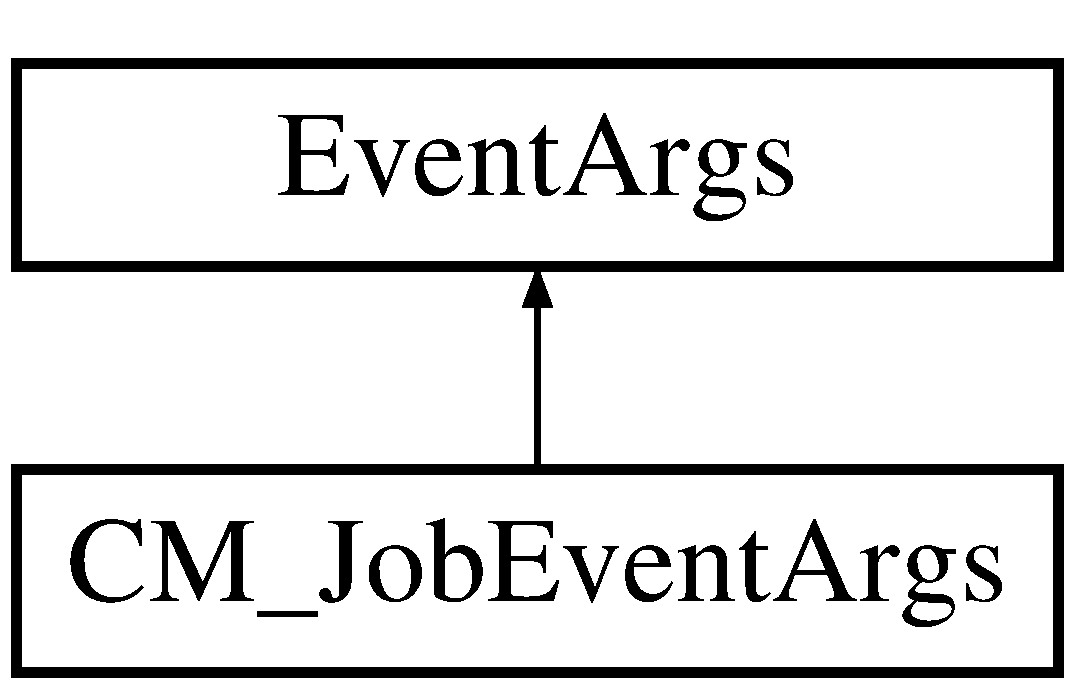
\includegraphics[height=2.000000cm]{class_c_m___job_event_args}
\end{center}
\end{figure}
\subsection*{Public Member Functions}
\begin{DoxyCompactItemize}
\item 
\hyperlink{class_c_m___job_event_args_a31a12f7cf24666f25f6b0967668cff61}{C\+M\+\_\+\+Job\+Event\+Args} (\hyperlink{class_c_m___job}{C\+M\+\_\+\+Job} \hyperlink{class_c_m___job_event_args_a602ecf7364ca2e6a2285f1622e7f1c8b}{job}, \hyperlink{class_c_m___job}{C\+M\+\_\+\+Job}\mbox{[}$\,$\mbox{]} \hyperlink{class_c_m___job_event_args_a6b20e99da0cb8807604b4459eebb4484}{child\+Jobs})
\begin{DoxyCompactList}\small\item\em Initializes a new instance of the \hyperlink{class_c_m___job_event_args}{C\+M\+\_\+\+Job\+Event\+Args} class. \end{DoxyCompactList}\end{DoxyCompactItemize}
\subsection*{Properties}
\begin{DoxyCompactItemize}
\item 
\hyperlink{class_c_m___job}{C\+M\+\_\+\+Job} \hyperlink{class_c_m___job_event_args_a602ecf7364ca2e6a2285f1622e7f1c8b}{job}\hspace{0.3cm}{\ttfamily  \mbox{[}get\mbox{]}}
\begin{DoxyCompactList}\small\item\em Gets the current job. \end{DoxyCompactList}\item 
\hyperlink{class_c_m___job}{C\+M\+\_\+\+Job}\mbox{[}$\,$\mbox{]} \hyperlink{class_c_m___job_event_args_a6b20e99da0cb8807604b4459eebb4484}{child\+Jobs}\hspace{0.3cm}{\ttfamily  \mbox{[}get\mbox{]}}
\begin{DoxyCompactList}\small\item\em Gets the child jobs (if any). \end{DoxyCompactList}\item 
bool \hyperlink{class_c_m___job_event_args_a67592931253f8d17df276bc17b54952b}{has\+Child\+Jobs}\hspace{0.3cm}{\ttfamily  \mbox{[}get\mbox{]}}
\begin{DoxyCompactList}\small\item\em Gets a value indicating whether this \hyperlink{class_c_m___job_event_args}{C\+M\+\_\+\+Job\+Event\+Args} has child jobs. \end{DoxyCompactList}\end{DoxyCompactItemize}


\subsection{Detailed Description}
Arguements used in events raised by \hyperlink{class_c_m___job}{C\+M\+\_\+\+Job}. 



\subsection{Constructor \& Destructor Documentation}
\hypertarget{class_c_m___job_event_args_a31a12f7cf24666f25f6b0967668cff61}{}\index{C\+M\+\_\+\+Job\+Event\+Args@{C\+M\+\_\+\+Job\+Event\+Args}!C\+M\+\_\+\+Job\+Event\+Args@{C\+M\+\_\+\+Job\+Event\+Args}}
\index{C\+M\+\_\+\+Job\+Event\+Args@{C\+M\+\_\+\+Job\+Event\+Args}!C\+M\+\_\+\+Job\+Event\+Args@{C\+M\+\_\+\+Job\+Event\+Args}}
\subsubsection[{C\+M\+\_\+\+Job\+Event\+Args(\+C\+M\+\_\+\+Job job, C\+M\+\_\+\+Job[] child\+Jobs)}]{\setlength{\rightskip}{0pt plus 5cm}C\+M\+\_\+\+Job\+Event\+Args.\+C\+M\+\_\+\+Job\+Event\+Args (
\begin{DoxyParamCaption}
\item[{{\bf C\+M\+\_\+\+Job}}]{job, }
\item[{{\bf C\+M\+\_\+\+Job}\mbox{[}$\,$\mbox{]}}]{child\+Jobs}
\end{DoxyParamCaption}
)}\label{class_c_m___job_event_args_a31a12f7cf24666f25f6b0967668cff61}


Initializes a new instance of the \hyperlink{class_c_m___job_event_args}{C\+M\+\_\+\+Job\+Event\+Args} class. 


\begin{DoxyParams}{Parameters}
{\em job} & Job.\\
\hline
{\em child\+Jobs} & Child jobs.\\
\hline
\end{DoxyParams}


\subsection{Property Documentation}
\hypertarget{class_c_m___job_event_args_a6b20e99da0cb8807604b4459eebb4484}{}\index{C\+M\+\_\+\+Job\+Event\+Args@{C\+M\+\_\+\+Job\+Event\+Args}!child\+Jobs@{child\+Jobs}}
\index{child\+Jobs@{child\+Jobs}!C\+M\+\_\+\+Job\+Event\+Args@{C\+M\+\_\+\+Job\+Event\+Args}}
\subsubsection[{child\+Jobs}]{\setlength{\rightskip}{0pt plus 5cm}{\bf C\+M\+\_\+\+Job} \mbox{[}$\,$\mbox{]} C\+M\+\_\+\+Job\+Event\+Args.\+child\+Jobs\hspace{0.3cm}{\ttfamily [get]}}\label{class_c_m___job_event_args_a6b20e99da0cb8807604b4459eebb4484}


Gets the child jobs (if any). 

The child jobs.\hypertarget{class_c_m___job_event_args_a67592931253f8d17df276bc17b54952b}{}\index{C\+M\+\_\+\+Job\+Event\+Args@{C\+M\+\_\+\+Job\+Event\+Args}!has\+Child\+Jobs@{has\+Child\+Jobs}}
\index{has\+Child\+Jobs@{has\+Child\+Jobs}!C\+M\+\_\+\+Job\+Event\+Args@{C\+M\+\_\+\+Job\+Event\+Args}}
\subsubsection[{has\+Child\+Jobs}]{\setlength{\rightskip}{0pt plus 5cm}bool C\+M\+\_\+\+Job\+Event\+Args.\+has\+Child\+Jobs\hspace{0.3cm}{\ttfamily [get]}}\label{class_c_m___job_event_args_a67592931253f8d17df276bc17b54952b}


Gets a value indicating whether this \hyperlink{class_c_m___job_event_args}{C\+M\+\_\+\+Job\+Event\+Args} has child jobs. 

{\ttfamily true} if has child jobs; otherwise, {\ttfamily false}.\hypertarget{class_c_m___job_event_args_a602ecf7364ca2e6a2285f1622e7f1c8b}{}\index{C\+M\+\_\+\+Job\+Event\+Args@{C\+M\+\_\+\+Job\+Event\+Args}!job@{job}}
\index{job@{job}!C\+M\+\_\+\+Job\+Event\+Args@{C\+M\+\_\+\+Job\+Event\+Args}}
\subsubsection[{job}]{\setlength{\rightskip}{0pt plus 5cm}{\bf C\+M\+\_\+\+Job} C\+M\+\_\+\+Job\+Event\+Args.\+job\hspace{0.3cm}{\ttfamily [get]}}\label{class_c_m___job_event_args_a602ecf7364ca2e6a2285f1622e7f1c8b}


Gets the current job. 

The job.

The documentation for this class was generated from the following file\+:\begin{DoxyCompactItemize}
\item 
C\+M\+\_\+\+Job\+Event\+Args.\+cs\end{DoxyCompactItemize}

\hypertarget{class_c_m___job_manager}{}\section{C\+M\+\_\+\+Job\+Manager Class Reference}
\label{class_c_m___job_manager}\index{C\+M\+\_\+\+Job\+Manager@{C\+M\+\_\+\+Job\+Manager}}


The main job manager class. Encapsulates the behaviour for global and local job managers. Provides access to events and public access to stored jobs.  


Inheritance diagram for C\+M\+\_\+\+Job\+Manager\+:\begin{figure}[H]
\begin{center}
\leavevmode
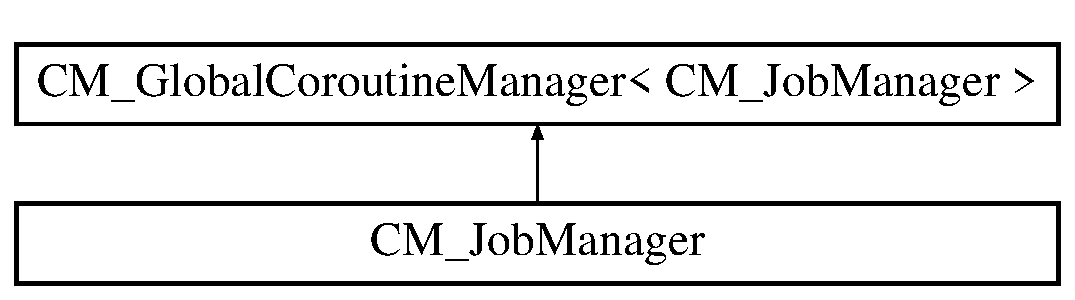
\includegraphics[height=2.000000cm]{class_c_m___job_manager}
\end{center}
\end{figure}
\subsection*{Public Member Functions}
\begin{DoxyCompactItemize}
\item 
\hyperlink{class_c_m___job_manager}{C\+M\+\_\+\+Job\+Manager} \hyperlink{class_c_m___job_manager_a3e8f2abdcaffd8f61f8a27be1b288c66}{Add\+Job} (\hyperlink{class_c_m___job}{C\+M\+\_\+\+Job} job)
\begin{DoxyCompactList}\small\item\em Adds a job to the job manager. \end{DoxyCompactList}\item 
\hyperlink{class_c_m___job_manager}{C\+M\+\_\+\+Job\+Manager} \hyperlink{class_c_m___job_manager_a03642325160354e27b9603b8e9b71996}{Add\+Job} (string id, I\+Enumerator routine)
\begin{DoxyCompactList}\small\item\em Creates a job with the specified id and routine and adds to job manager. \end{DoxyCompactList}\item 
\hyperlink{class_c_m___job_manager}{C\+M\+\_\+\+Job\+Manager} \hyperlink{class_c_m___job_manager_a3c8aef4596141686e60e5a3166c7264a}{Add\+Job} (I\+List$<$ \hyperlink{class_c_m___job}{C\+M\+\_\+\+Job} $>$ jobs)
\begin{DoxyCompactList}\small\item\em Adds the provided jobs to the job manager. \end{DoxyCompactList}\item 
\hyperlink{class_c_m___job_manager}{C\+M\+\_\+\+Job\+Manager} \hyperlink{class_c_m___job_manager_a295f3f6cd5f10cc3646f6f85203097f6}{Add\+Job} (params \hyperlink{class_c_m___job}{C\+M\+\_\+\+Job}\mbox{[}$\,$\mbox{]} jobs)
\begin{DoxyCompactList}\small\item\em Adds the provided jobs to the job manager. \end{DoxyCompactList}\item 
\hyperlink{class_c_m___job_manager}{C\+M\+\_\+\+Job\+Manager} \hyperlink{class_c_m___job_manager_a70e6b6c8c3252c52549123df98349db4}{Remove\+Job} (\hyperlink{class_c_m___job}{C\+M\+\_\+\+Job} job)
\begin{DoxyCompactList}\small\item\em Removes the job if owned by this instance of job manager. \end{DoxyCompactList}\item 
\hyperlink{class_c_m___job_manager}{C\+M\+\_\+\+Job\+Manager} \hyperlink{class_c_m___job_manager_afc719b10d34b02fa82c26bbfbadc7356}{Remove\+Job} (string id)
\begin{DoxyCompactList}\small\item\em Removes the job if owned by this instance of job manager. \end{DoxyCompactList}\item 
\hyperlink{class_c_m___job_manager}{C\+M\+\_\+\+Job\+Manager} \hyperlink{class_c_m___job_manager_a81deb518cf6f4359330e6f0d405080ef}{Start\+Coroutine} (\hyperlink{class_c_m___job}{C\+M\+\_\+\+Job} job)
\begin{DoxyCompactList}\small\item\em Starts the specified coroutine if owned by this instance of job manager. Job is searched using job id. \end{DoxyCompactList}\item 
\hyperlink{class_c_m___job_manager}{C\+M\+\_\+\+Job\+Manager} \hyperlink{class_c_m___job_manager_af2bb3415fd6f85c1e04f99b2cc6efd4e}{Start\+Coroutine} (string id)
\begin{DoxyCompactList}\small\item\em Starts the specified coroutine if owned by this instance of job manager. \end{DoxyCompactList}\item 
\hyperlink{class_c_m___job_manager}{C\+M\+\_\+\+Job\+Manager} \hyperlink{class_c_m___job_manager_aeee478b4e96e09cb9f4a7e3610c7dd49}{Start\+All} ()
\begin{DoxyCompactList}\small\item\em Starts all jobs owned by this instance. \end{DoxyCompactList}\item 
\hyperlink{class_c_m___job_manager}{C\+M\+\_\+\+Job\+Manager} \hyperlink{class_c_m___job_manager_acf6ad4a995461c0bc6f519150e57306c}{Start\+All} (float delay\+In\+Seconds)
\begin{DoxyCompactList}\small\item\em Starts all jobs owned by this instance after delay in seconds. \end{DoxyCompactList}\item 
\hyperlink{class_c_m___job_manager}{C\+M\+\_\+\+Job\+Manager} \hyperlink{class_c_m___job_manager_adf2ecaac62cbb5f946c6644dc03bc69c}{Stop\+Coroutine} (\hyperlink{class_c_m___job}{C\+M\+\_\+\+Job} job)
\begin{DoxyCompactList}\small\item\em Stops the specified coroutine if owned by this instance of job manager. Job is searched using job id. \end{DoxyCompactList}\item 
\hyperlink{class_c_m___job_manager}{C\+M\+\_\+\+Job\+Manager} \hyperlink{class_c_m___job_manager_ae5f0aba4e929269d10659a7b19579b7d}{Stop\+Coroutine} (string id)
\begin{DoxyCompactList}\small\item\em Stops the specified coroutine if owned by this instance of job manager. \end{DoxyCompactList}\item 
\hyperlink{class_c_m___job_manager}{C\+M\+\_\+\+Job\+Manager} \hyperlink{class_c_m___job_manager_a4d5891acec719e1003dc762df52a931a}{Pause\+Coroutine} (\hyperlink{class_c_m___job}{C\+M\+\_\+\+Job} job)
\begin{DoxyCompactList}\small\item\em Pauses the specified coroutine if owned by this instance of job manager. Job is searched using job id. \end{DoxyCompactList}\item 
\hyperlink{class_c_m___job_manager}{C\+M\+\_\+\+Job\+Manager} \hyperlink{class_c_m___job_manager_ae04090c1ecd34beb61a00f44d239b5f7}{Pause\+Coroutine} (string id)
\begin{DoxyCompactList}\small\item\em Stops the specified coroutine if owned by this instance of job manager. \end{DoxyCompactList}\item 
\hyperlink{class_c_m___job_manager}{C\+M\+\_\+\+Job\+Manager} \hyperlink{class_c_m___job_manager_a18f956a6db3fe89f4597c317838ab073}{Resume\+Coroutine} (\hyperlink{class_c_m___job}{C\+M\+\_\+\+Job} job)
\begin{DoxyCompactList}\small\item\em Resumes the specified coroutine if owned by this instance of job manager. Job is searched using job id. \end{DoxyCompactList}\item 
\hyperlink{class_c_m___job_manager}{C\+M\+\_\+\+Job\+Manager} \hyperlink{class_c_m___job_manager_a4038c3f395f2a64c3b4e18680d0a50ef}{Resume\+Coroutine} (string id)
\begin{DoxyCompactList}\small\item\em Stops the specified coroutine if owned by this instance of job manager. \end{DoxyCompactList}\item 
\hyperlink{class_c_m___job_manager}{C\+M\+\_\+\+Job\+Manager} \hyperlink{class_c_m___job_manager_ab1e48755bb929871595acfca595ae01b}{Pause\+All} ()
\begin{DoxyCompactList}\small\item\em Pauses all jobs owned by this instance. Raises all\+Jobs\+Paused event. \end{DoxyCompactList}\item 
\hyperlink{class_c_m___job_manager}{C\+M\+\_\+\+Job\+Manager} \hyperlink{class_c_m___job_manager_a32a5f874cae07a572b5f5115c48fc528}{Pause\+All} (float delay\+In\+Seconds)
\begin{DoxyCompactList}\small\item\em Pauses all jobs owned by this instance after delay in seconds. Raises all\+Jobs\+Paused event. \end{DoxyCompactList}\item 
\hyperlink{class_c_m___job_manager}{C\+M\+\_\+\+Job\+Manager} \hyperlink{class_c_m___job_manager_a838152b138f04a0c4c254f3b56bd31fe}{Resume\+All} ()
\begin{DoxyCompactList}\small\item\em Resumes all jobs owned by this instance. Raises all\+Jobs\+Resumed\+Event. \end{DoxyCompactList}\item 
\hyperlink{class_c_m___job_manager}{C\+M\+\_\+\+Job\+Manager} \hyperlink{class_c_m___job_manager_ac87588d5764ca7a71208ff96f3fd67f7}{Resume\+All} (float delay\+In\+Seconds)
\begin{DoxyCompactList}\small\item\em Resumes all jobs owned by this instance after delay in seconds. Raises all\+Jobs\+Resumed\+Event. \end{DoxyCompactList}\item 
\hyperlink{class_c_m___job_manager}{C\+M\+\_\+\+Job\+Manager} \hyperlink{class_c_m___job_manager_ab5a27b84b4fd3893e1dc271570930e62}{Kill\+All} ()
\begin{DoxyCompactList}\small\item\em Kills all jobs owned by this instance. Raises all\+Jobs\+Killed event. \end{DoxyCompactList}\item 
\hyperlink{class_c_m___job_manager}{C\+M\+\_\+\+Job\+Manager} \hyperlink{class_c_m___job_manager_a6c81a2ea2ade217311fef98c4571e9e5}{Kill\+All} (float delay\+In\+Seconds)
\begin{DoxyCompactList}\small\item\em Kills all jobs owned by this instance after delay in seconds. Raises all\+Jobs\+Killed event. \end{DoxyCompactList}\item 
\hyperlink{class_c_m___job_manager}{C\+M\+\_\+\+Job\+Manager} \hyperlink{class_c_m___job_manager_a7684d8a980b6dd3004feb35e978e2163}{Clear\+Job\+List} ()
\begin{DoxyCompactList}\small\item\em Clears the job list owned by this instance. It does not kill the jobs so they will continue to run. Raises all\+Jobs\+Cleared event. \end{DoxyCompactList}\item 
bool \hyperlink{class_c_m___job_manager_a5b18579964f7e16836eb66465c4f6d09}{Has\+Job} (string id)
\begin{DoxyCompactList}\small\item\em Determines whether this instance has the job with the specified id. \end{DoxyCompactList}\item 
bool \hyperlink{class_c_m___job_manager_a12642c18c8755585be14a1566a000113}{Is\+Running} (\hyperlink{class_c_m___job}{C\+M\+\_\+\+Job} job)
\begin{DoxyCompactList}\small\item\em Determines whether the specified job is executing. \end{DoxyCompactList}\item 
bool \hyperlink{class_c_m___job_manager_a5a3b38ca378a94e24e39a111734d9791}{Is\+Running} (string id)
\begin{DoxyCompactList}\small\item\em Determines whether the specified job is executing. \end{DoxyCompactList}\item 
\hyperlink{class_c_m___job_manager}{C\+M\+\_\+\+Job\+Manager} \hyperlink{class_c_m___job_manager_a00224b541cd09c65942f7b23ee0b39c0}{Notify\+On\+Job\+Added} (Event\+Handler$<$ \hyperlink{class_c_m___job_manager_job_edited_event_args}{C\+M\+\_\+\+Job\+Manager\+Job\+Edited\+Event\+Args} $>$ e)
\begin{DoxyCompactList}\small\item\em Subscribes to the the job\+Added event. \end{DoxyCompactList}\item 
\hyperlink{class_c_m___job_manager}{C\+M\+\_\+\+Job\+Manager} \hyperlink{class_c_m___job_manager_acd3196581bb9e192e05274fca2e27cdc}{Remove\+Notify\+On\+Job\+Added} (Event\+Handler$<$ \hyperlink{class_c_m___job_manager_job_edited_event_args}{C\+M\+\_\+\+Job\+Manager\+Job\+Edited\+Event\+Args} $>$ e)
\begin{DoxyCompactList}\small\item\em Unsubscribes to the the job\+Added event. \end{DoxyCompactList}\item 
\hyperlink{class_c_m___job_manager}{C\+M\+\_\+\+Job\+Manager} \hyperlink{class_c_m___job_manager_afcf02b75d90366cecc51bc9d3dba518d}{Notify\+On\+Job\+Removed} (Event\+Handler$<$ \hyperlink{class_c_m___job_manager_job_edited_event_args}{C\+M\+\_\+\+Job\+Manager\+Job\+Edited\+Event\+Args} $>$ e)
\begin{DoxyCompactList}\small\item\em Subscribes to the the job\+Removed event. \end{DoxyCompactList}\item 
\hyperlink{class_c_m___job_manager}{C\+M\+\_\+\+Job\+Manager} \hyperlink{class_c_m___job_manager_abbe42e2c33064edd8d43148ef8ce6df6}{Remove\+Notify\+On\+Job\+Removed} (Event\+Handler$<$ \hyperlink{class_c_m___job_manager_job_edited_event_args}{C\+M\+\_\+\+Job\+Manager\+Job\+Edited\+Event\+Args} $>$ e)
\begin{DoxyCompactList}\small\item\em Unsubscribes to the the job\+Removed event. \end{DoxyCompactList}\item 
\hyperlink{class_c_m___job_manager}{C\+M\+\_\+\+Job\+Manager} \hyperlink{class_c_m___job_manager_a5818cc96746d71cd81bcf711047ca360}{Notify\+On\+All\+Jobs\+Paused} (Event\+Handler$<$ \hyperlink{class_c_m___job_manager_event_args}{C\+M\+\_\+\+Job\+Manager\+Event\+Args} $>$ e)
\begin{DoxyCompactList}\small\item\em Subscribes to the the job\+Paused event. \end{DoxyCompactList}\item 
\hyperlink{class_c_m___job_manager}{C\+M\+\_\+\+Job\+Manager} \hyperlink{class_c_m___job_manager_a6399741e966f8f613b0dc97438263d8c}{Remove\+Notify\+On\+All\+Jobs\+Paused} (Event\+Handler$<$ \hyperlink{class_c_m___job_manager_event_args}{C\+M\+\_\+\+Job\+Manager\+Event\+Args} $>$ e)
\begin{DoxyCompactList}\small\item\em Unsubscribes to the the job\+Paused event. \end{DoxyCompactList}\item 
\hyperlink{class_c_m___job_manager}{C\+M\+\_\+\+Job\+Manager} \hyperlink{class_c_m___job_manager_a940976b91755f7849232bad8b6fdd472}{Notify\+On\+All\+Jobs\+Resumed} (Event\+Handler$<$ \hyperlink{class_c_m___job_manager_event_args}{C\+M\+\_\+\+Job\+Manager\+Event\+Args} $>$ e)
\begin{DoxyCompactList}\small\item\em Subscribes to the the job\+Resumed event. \end{DoxyCompactList}\item 
\hyperlink{class_c_m___job_manager}{C\+M\+\_\+\+Job\+Manager} \hyperlink{class_c_m___job_manager_aac35272ab72db1d666bca8e9825af345}{Remove\+Notify\+On\+All\+Jobs\+Resumed} (Event\+Handler$<$ \hyperlink{class_c_m___job_manager_event_args}{C\+M\+\_\+\+Job\+Manager\+Event\+Args} $>$ e)
\begin{DoxyCompactList}\small\item\em Unsubscribes to the the job\+Resumed event. \end{DoxyCompactList}\item 
\hyperlink{class_c_m___job_manager}{C\+M\+\_\+\+Job\+Manager} \hyperlink{class_c_m___job_manager_a047fad74154dfb0dfd95b2e68c241c53}{Notify\+On\+All\+Jobs\+Killed} (Event\+Handler$<$ \hyperlink{class_c_m___job_manager_event_args}{C\+M\+\_\+\+Job\+Manager\+Event\+Args} $>$ e)
\begin{DoxyCompactList}\small\item\em Subscribes to the the all\+Jobs\+Killed event. \end{DoxyCompactList}\item 
\hyperlink{class_c_m___job_manager}{C\+M\+\_\+\+Job\+Manager} \hyperlink{class_c_m___job_manager_a86d91437f2588d7f218ced31689bfbcd}{Remove\+Notify\+On\+All\+Jobs\+Killed} (Event\+Handler$<$ \hyperlink{class_c_m___job_manager_event_args}{C\+M\+\_\+\+Job\+Manager\+Event\+Args} $>$ e)
\begin{DoxyCompactList}\small\item\em Unsubscribes to the the all\+Jobs\+Killed event. \end{DoxyCompactList}\item 
\hyperlink{class_c_m___job_manager}{C\+M\+\_\+\+Job\+Manager} \hyperlink{class_c_m___job_manager_a61b1d9a2f93539f35a65bc52f35a2a7d}{Notify\+On\+All\+Jobs\+Cleared} (Event\+Handler$<$ \hyperlink{class_c_m___job_manager_event_args}{C\+M\+\_\+\+Job\+Manager\+Event\+Args} $>$ e)
\begin{DoxyCompactList}\small\item\em Subscribes to the the all\+Jobs\+Cleared event. \end{DoxyCompactList}\item 
\hyperlink{class_c_m___job_manager}{C\+M\+\_\+\+Job\+Manager} \hyperlink{class_c_m___job_manager_addf2ff8338d0cef43d47c8f0c95ec7c1}{Remove\+Notify\+On\+All\+Jobs\+Cleared} (Event\+Handler$<$ \hyperlink{class_c_m___job_manager_event_args}{C\+M\+\_\+\+Job\+Manager\+Event\+Args} $>$ e)
\begin{DoxyCompactList}\small\item\em Unsubscribes to the the all\+Jobs\+Cleared event. \end{DoxyCompactList}\item 
void \hyperlink{class_c_m___job_manager_a26be7a4d45e34639bde44ec8c7a7dac4}{On\+Job\+Removed} (\hyperlink{class_c_m___job_manager_job_edited_event_args}{C\+M\+\_\+\+Job\+Manager\+Job\+Edited\+Event\+Args} e)
\begin{DoxyCompactList}\small\item\em Raises the job removed event. \end{DoxyCompactList}\item 
void \hyperlink{class_c_m___job_manager_ae6f76e1db2269e63506ad70d063e6fd0}{On\+All\+Jobs\+Resumed} (\hyperlink{class_c_m___job_manager_event_args}{C\+M\+\_\+\+Job\+Manager\+Event\+Args} e)
\begin{DoxyCompactList}\small\item\em Raises the all jobs resumed event. \end{DoxyCompactList}\item 
void \hyperlink{class_c_m___job_manager_ae666d35da523c26313933b7b9c9ca244}{On\+All\+Jobs\+Paused} (\hyperlink{class_c_m___job_manager_event_args}{C\+M\+\_\+\+Job\+Manager\+Event\+Args} e)
\begin{DoxyCompactList}\small\item\em Raises the all jobs paused event. \end{DoxyCompactList}\item 
void \hyperlink{class_c_m___job_manager_a8aafc682e991a7b2c8cf056292243db8}{On\+All\+Jobs\+Killed} (\hyperlink{class_c_m___job_manager_event_args}{C\+M\+\_\+\+Job\+Manager\+Event\+Args} e)
\begin{DoxyCompactList}\small\item\em Raises the all jobs killed event. \end{DoxyCompactList}\item 
void \hyperlink{class_c_m___job_manager_ab7c334ef31635981f63460e5f8b270bf}{On\+All\+Jobs\+Cleared} (\hyperlink{class_c_m___job_manager_event_args}{C\+M\+\_\+\+Job\+Manager\+Event\+Args} e)
\begin{DoxyCompactList}\small\item\em Raises the all jobs cleared event. \end{DoxyCompactList}\end{DoxyCompactItemize}
\subsection*{Static Public Member Functions}
\begin{DoxyCompactItemize}
\item 
static \hyperlink{class_c_m___job_manager}{C\+M\+\_\+\+Job\+Manager} \hyperlink{class_c_m___job_manager_a404b217320793549dca8cd2c5914c608}{Make} ()
\begin{DoxyCompactList}\small\item\em Returns an initialised \hyperlink{class_c_m___job_manager}{C\+M\+\_\+\+Job\+Manager} instance. Provides static access to class. \end{DoxyCompactList}\end{DoxyCompactItemize}
\subsection*{Protected Member Functions}
\begin{DoxyCompactItemize}
\item 
void \hyperlink{class_c_m___job_manager_ae64a14d83bc4c6e0634b6469edbbef03}{On\+Job\+Added} (\hyperlink{class_c_m___job_manager_job_edited_event_args}{C\+M\+\_\+\+Job\+Manager\+Job\+Edited\+Event\+Args} e)
\begin{DoxyCompactList}\small\item\em Raises the job added event. \end{DoxyCompactList}\item 
\hypertarget{class_c_m___job_manager_a0c5d0104abdf10bda6af89301376792b}{}override void {\bfseries Handlejob\+Complete} (object sender, \hyperlink{class_c_m___job_event_args}{C\+M\+\_\+\+Job\+Event\+Args} e)\label{class_c_m___job_manager_a0c5d0104abdf10bda6af89301376792b}

\end{DoxyCompactItemize}
\subsection*{Events}
\begin{DoxyCompactItemize}
\item 
Event\+Handler$<$ \hyperlink{class_c_m___job_manager_job_edited_event_args}{C\+M\+\_\+\+Job\+Manager\+Job\+Edited\+Event\+Args} $>$ \hyperlink{class_c_m___job_manager_a0f3c4dff8b782e1b64abcbb7dc19cd8a}{job\+Added}
\begin{DoxyCompactList}\small\item\em Raised when job added. \end{DoxyCompactList}\item 
Event\+Handler$<$ \hyperlink{class_c_m___job_manager_job_edited_event_args}{C\+M\+\_\+\+Job\+Manager\+Job\+Edited\+Event\+Args} $>$ \hyperlink{class_c_m___job_manager_a3a24d267ce0e6a09a2cf8f13429f2b73}{job\+Removed}
\begin{DoxyCompactList}\small\item\em Raised when job removed. \end{DoxyCompactList}\item 
Event\+Handler$<$ \hyperlink{class_c_m___job_manager_event_args}{C\+M\+\_\+\+Job\+Manager\+Event\+Args} $>$ \hyperlink{class_c_m___job_manager_ac17ba0c89adf4dfa61d6b099f8029fa6}{all\+Jobs\+Killed}
\begin{DoxyCompactList}\small\item\em Raised when all jobs killed. \end{DoxyCompactList}\item 
Event\+Handler$<$ \hyperlink{class_c_m___job_manager_event_args}{C\+M\+\_\+\+Job\+Manager\+Event\+Args} $>$ \hyperlink{class_c_m___job_manager_a485232e2c1fe7cef56a53c20f74b638f}{all\+Jobs\+Resumed}
\begin{DoxyCompactList}\small\item\em Raised when all jobs resumed. \end{DoxyCompactList}\item 
Event\+Handler$<$ \hyperlink{class_c_m___job_manager_event_args}{C\+M\+\_\+\+Job\+Manager\+Event\+Args} $>$ \hyperlink{class_c_m___job_manager_a0dd6f2e0e4c7ead23dd25df03e23ddcb}{all\+Jobs\+Paused}
\begin{DoxyCompactList}\small\item\em Raised when all jobs paused. \end{DoxyCompactList}\item 
Event\+Handler$<$ \hyperlink{class_c_m___job_manager_event_args}{C\+M\+\_\+\+Job\+Manager\+Event\+Args} $>$ \hyperlink{class_c_m___job_manager_a292061e968b70d3271715d7a1c702db1}{all\+Jobs\+Cleared}
\begin{DoxyCompactList}\small\item\em Raised when all jobs cleared. \end{DoxyCompactList}\end{DoxyCompactItemize}
\subsection*{Additional Inherited Members}


\subsection{Detailed Description}
The main job manager class. Encapsulates the behaviour for global and local job managers. Provides access to events and public access to stored jobs. 



\subsection{Member Function Documentation}
\hypertarget{class_c_m___job_manager_a3e8f2abdcaffd8f61f8a27be1b288c66}{}\index{C\+M\+\_\+\+Job\+Manager@{C\+M\+\_\+\+Job\+Manager}!Add\+Job@{Add\+Job}}
\index{Add\+Job@{Add\+Job}!C\+M\+\_\+\+Job\+Manager@{C\+M\+\_\+\+Job\+Manager}}
\subsubsection[{Add\+Job(\+C\+M\+\_\+\+Job job)}]{\setlength{\rightskip}{0pt plus 5cm}{\bf C\+M\+\_\+\+Job\+Manager} C\+M\+\_\+\+Job\+Manager.\+Add\+Job (
\begin{DoxyParamCaption}
\item[{{\bf C\+M\+\_\+\+Job}}]{job}
\end{DoxyParamCaption}
)}\label{class_c_m___job_manager_a3e8f2abdcaffd8f61f8a27be1b288c66}


Adds a job to the job manager. 

\begin{DoxyReturn}{Returns}
The job.
\end{DoxyReturn}

\begin{DoxyParams}{Parameters}
{\em job} & Job.\\
\hline
\end{DoxyParams}
\hypertarget{class_c_m___job_manager_a03642325160354e27b9603b8e9b71996}{}\index{C\+M\+\_\+\+Job\+Manager@{C\+M\+\_\+\+Job\+Manager}!Add\+Job@{Add\+Job}}
\index{Add\+Job@{Add\+Job}!C\+M\+\_\+\+Job\+Manager@{C\+M\+\_\+\+Job\+Manager}}
\subsubsection[{Add\+Job(string id, I\+Enumerator routine)}]{\setlength{\rightskip}{0pt plus 5cm}{\bf C\+M\+\_\+\+Job\+Manager} C\+M\+\_\+\+Job\+Manager.\+Add\+Job (
\begin{DoxyParamCaption}
\item[{string}]{id, }
\item[{I\+Enumerator}]{routine}
\end{DoxyParamCaption}
)}\label{class_c_m___job_manager_a03642325160354e27b9603b8e9b71996}


Creates a job with the specified id and routine and adds to job manager. 

\begin{DoxyReturn}{Returns}
The job manager.
\end{DoxyReturn}

\begin{DoxyParams}{Parameters}
{\em id} & Identifier of job.\\
\hline
{\em routine} & Routine.\\
\hline
\end{DoxyParams}
\hypertarget{class_c_m___job_manager_a3c8aef4596141686e60e5a3166c7264a}{}\index{C\+M\+\_\+\+Job\+Manager@{C\+M\+\_\+\+Job\+Manager}!Add\+Job@{Add\+Job}}
\index{Add\+Job@{Add\+Job}!C\+M\+\_\+\+Job\+Manager@{C\+M\+\_\+\+Job\+Manager}}
\subsubsection[{Add\+Job(\+I\+List$<$ C\+M\+\_\+\+Job $>$ jobs)}]{\setlength{\rightskip}{0pt plus 5cm}{\bf C\+M\+\_\+\+Job\+Manager} C\+M\+\_\+\+Job\+Manager.\+Add\+Job (
\begin{DoxyParamCaption}
\item[{I\+List$<$ {\bf C\+M\+\_\+\+Job} $>$}]{jobs}
\end{DoxyParamCaption}
)}\label{class_c_m___job_manager_a3c8aef4596141686e60e5a3166c7264a}


Adds the provided jobs to the job manager. 

\begin{DoxyReturn}{Returns}
The job manager.
\end{DoxyReturn}

\begin{DoxyParams}{Parameters}
{\em jobs} & Jobs to add to this instance.\\
\hline
\end{DoxyParams}
\hypertarget{class_c_m___job_manager_a295f3f6cd5f10cc3646f6f85203097f6}{}\index{C\+M\+\_\+\+Job\+Manager@{C\+M\+\_\+\+Job\+Manager}!Add\+Job@{Add\+Job}}
\index{Add\+Job@{Add\+Job}!C\+M\+\_\+\+Job\+Manager@{C\+M\+\_\+\+Job\+Manager}}
\subsubsection[{Add\+Job(params C\+M\+\_\+\+Job[] jobs)}]{\setlength{\rightskip}{0pt plus 5cm}{\bf C\+M\+\_\+\+Job\+Manager} C\+M\+\_\+\+Job\+Manager.\+Add\+Job (
\begin{DoxyParamCaption}
\item[{params {\bf C\+M\+\_\+\+Job}\mbox{[}$\,$\mbox{]}}]{jobs}
\end{DoxyParamCaption}
)}\label{class_c_m___job_manager_a295f3f6cd5f10cc3646f6f85203097f6}


Adds the provided jobs to the job manager. 

\begin{DoxyReturn}{Returns}
The job manager.
\end{DoxyReturn}

\begin{DoxyParams}{Parameters}
{\em jobs} & Jobs to add to this instance.\\
\hline
\end{DoxyParams}
\hypertarget{class_c_m___job_manager_a7684d8a980b6dd3004feb35e978e2163}{}\index{C\+M\+\_\+\+Job\+Manager@{C\+M\+\_\+\+Job\+Manager}!Clear\+Job\+List@{Clear\+Job\+List}}
\index{Clear\+Job\+List@{Clear\+Job\+List}!C\+M\+\_\+\+Job\+Manager@{C\+M\+\_\+\+Job\+Manager}}
\subsubsection[{Clear\+Job\+List()}]{\setlength{\rightskip}{0pt plus 5cm}{\bf C\+M\+\_\+\+Job\+Manager} C\+M\+\_\+\+Job\+Manager.\+Clear\+Job\+List (
\begin{DoxyParamCaption}
{}
\end{DoxyParamCaption}
)}\label{class_c_m___job_manager_a7684d8a980b6dd3004feb35e978e2163}


Clears the job list owned by this instance. It does not kill the jobs so they will continue to run. Raises all\+Jobs\+Cleared event. 

\begin{DoxyReturn}{Returns}
The job list.
\end{DoxyReturn}
\hypertarget{class_c_m___job_manager_a5b18579964f7e16836eb66465c4f6d09}{}\index{C\+M\+\_\+\+Job\+Manager@{C\+M\+\_\+\+Job\+Manager}!Has\+Job@{Has\+Job}}
\index{Has\+Job@{Has\+Job}!C\+M\+\_\+\+Job\+Manager@{C\+M\+\_\+\+Job\+Manager}}
\subsubsection[{Has\+Job(string id)}]{\setlength{\rightskip}{0pt plus 5cm}bool C\+M\+\_\+\+Job\+Manager.\+Has\+Job (
\begin{DoxyParamCaption}
\item[{string}]{id}
\end{DoxyParamCaption}
)}\label{class_c_m___job_manager_a5b18579964f7e16836eb66465c4f6d09}


Determines whether this instance has the job with the specified id. 

\begin{DoxyReturn}{Returns}
{\ttfamily true} if this instance has a job with the specified id; otherwise, {\ttfamily false}.
\end{DoxyReturn}

\begin{DoxyParams}{Parameters}
{\em id} & Identifier.\\
\hline
\end{DoxyParams}
\hypertarget{class_c_m___job_manager_a12642c18c8755585be14a1566a000113}{}\index{C\+M\+\_\+\+Job\+Manager@{C\+M\+\_\+\+Job\+Manager}!Is\+Running@{Is\+Running}}
\index{Is\+Running@{Is\+Running}!C\+M\+\_\+\+Job\+Manager@{C\+M\+\_\+\+Job\+Manager}}
\subsubsection[{Is\+Running(\+C\+M\+\_\+\+Job job)}]{\setlength{\rightskip}{0pt plus 5cm}bool C\+M\+\_\+\+Job\+Manager.\+Is\+Running (
\begin{DoxyParamCaption}
\item[{{\bf C\+M\+\_\+\+Job}}]{job}
\end{DoxyParamCaption}
)}\label{class_c_m___job_manager_a12642c18c8755585be14a1566a000113}


Determines whether the specified job is executing. 

\begin{DoxyReturn}{Returns}
{\ttfamily true} if the job is currently running; otherwise, {\ttfamily false}.
\end{DoxyReturn}

\begin{DoxyParams}{Parameters}
{\em job} & Job.\\
\hline
\end{DoxyParams}
\hypertarget{class_c_m___job_manager_a5a3b38ca378a94e24e39a111734d9791}{}\index{C\+M\+\_\+\+Job\+Manager@{C\+M\+\_\+\+Job\+Manager}!Is\+Running@{Is\+Running}}
\index{Is\+Running@{Is\+Running}!C\+M\+\_\+\+Job\+Manager@{C\+M\+\_\+\+Job\+Manager}}
\subsubsection[{Is\+Running(string id)}]{\setlength{\rightskip}{0pt plus 5cm}bool C\+M\+\_\+\+Job\+Manager.\+Is\+Running (
\begin{DoxyParamCaption}
\item[{string}]{id}
\end{DoxyParamCaption}
)}\label{class_c_m___job_manager_a5a3b38ca378a94e24e39a111734d9791}


Determines whether the specified job is executing. 

\begin{DoxyReturn}{Returns}
{\ttfamily true} if the job is currently running; otherwise, {\ttfamily false}.
\end{DoxyReturn}

\begin{DoxyParams}{Parameters}
{\em job} & Job I\+D.\\
\hline
\end{DoxyParams}
\hypertarget{class_c_m___job_manager_ab5a27b84b4fd3893e1dc271570930e62}{}\index{C\+M\+\_\+\+Job\+Manager@{C\+M\+\_\+\+Job\+Manager}!Kill\+All@{Kill\+All}}
\index{Kill\+All@{Kill\+All}!C\+M\+\_\+\+Job\+Manager@{C\+M\+\_\+\+Job\+Manager}}
\subsubsection[{Kill\+All()}]{\setlength{\rightskip}{0pt plus 5cm}{\bf C\+M\+\_\+\+Job\+Manager} C\+M\+\_\+\+Job\+Manager.\+Kill\+All (
\begin{DoxyParamCaption}
{}
\end{DoxyParamCaption}
)}\label{class_c_m___job_manager_ab5a27b84b4fd3893e1dc271570930e62}


Kills all jobs owned by this instance. Raises all\+Jobs\+Killed event. 

\begin{DoxyReturn}{Returns}
The all.
\end{DoxyReturn}
\hypertarget{class_c_m___job_manager_a6c81a2ea2ade217311fef98c4571e9e5}{}\index{C\+M\+\_\+\+Job\+Manager@{C\+M\+\_\+\+Job\+Manager}!Kill\+All@{Kill\+All}}
\index{Kill\+All@{Kill\+All}!C\+M\+\_\+\+Job\+Manager@{C\+M\+\_\+\+Job\+Manager}}
\subsubsection[{Kill\+All(float delay\+In\+Seconds)}]{\setlength{\rightskip}{0pt plus 5cm}{\bf C\+M\+\_\+\+Job\+Manager} C\+M\+\_\+\+Job\+Manager.\+Kill\+All (
\begin{DoxyParamCaption}
\item[{float}]{delay\+In\+Seconds}
\end{DoxyParamCaption}
)}\label{class_c_m___job_manager_a6c81a2ea2ade217311fef98c4571e9e5}


Kills all jobs owned by this instance after delay in seconds. Raises all\+Jobs\+Killed event. 

\begin{DoxyReturn}{Returns}
The all.
\end{DoxyReturn}

\begin{DoxyParams}{Parameters}
{\em delay\+In\+Seconds} & Delay in seconds.\\
\hline
\end{DoxyParams}
\hypertarget{class_c_m___job_manager_a404b217320793549dca8cd2c5914c608}{}\index{C\+M\+\_\+\+Job\+Manager@{C\+M\+\_\+\+Job\+Manager}!Make@{Make}}
\index{Make@{Make}!C\+M\+\_\+\+Job\+Manager@{C\+M\+\_\+\+Job\+Manager}}
\subsubsection[{Make()}]{\setlength{\rightskip}{0pt plus 5cm}static {\bf C\+M\+\_\+\+Job\+Manager} C\+M\+\_\+\+Job\+Manager.\+Make (
\begin{DoxyParamCaption}
{}
\end{DoxyParamCaption}
)\hspace{0.3cm}{\ttfamily [static]}}\label{class_c_m___job_manager_a404b217320793549dca8cd2c5914c608}


Returns an initialised \hyperlink{class_c_m___job_manager}{C\+M\+\_\+\+Job\+Manager} instance. Provides static access to class. 

\hypertarget{class_c_m___job_manager_a61b1d9a2f93539f35a65bc52f35a2a7d}{}\index{C\+M\+\_\+\+Job\+Manager@{C\+M\+\_\+\+Job\+Manager}!Notify\+On\+All\+Jobs\+Cleared@{Notify\+On\+All\+Jobs\+Cleared}}
\index{Notify\+On\+All\+Jobs\+Cleared@{Notify\+On\+All\+Jobs\+Cleared}!C\+M\+\_\+\+Job\+Manager@{C\+M\+\_\+\+Job\+Manager}}
\subsubsection[{Notify\+On\+All\+Jobs\+Cleared(\+Event\+Handler$<$ C\+M\+\_\+\+Job\+Manager\+Event\+Args $>$ e)}]{\setlength{\rightskip}{0pt plus 5cm}{\bf C\+M\+\_\+\+Job\+Manager} C\+M\+\_\+\+Job\+Manager.\+Notify\+On\+All\+Jobs\+Cleared (
\begin{DoxyParamCaption}
\item[{Event\+Handler$<$ {\bf C\+M\+\_\+\+Job\+Manager\+Event\+Args} $>$}]{e}
\end{DoxyParamCaption}
)}\label{class_c_m___job_manager_a61b1d9a2f93539f35a65bc52f35a2a7d}


Subscribes to the the all\+Jobs\+Cleared event. 


\begin{DoxyParams}{Parameters}
{\em e} & The eventhandler to be invoked on event.\\
\hline
\end{DoxyParams}
\hypertarget{class_c_m___job_manager_a047fad74154dfb0dfd95b2e68c241c53}{}\index{C\+M\+\_\+\+Job\+Manager@{C\+M\+\_\+\+Job\+Manager}!Notify\+On\+All\+Jobs\+Killed@{Notify\+On\+All\+Jobs\+Killed}}
\index{Notify\+On\+All\+Jobs\+Killed@{Notify\+On\+All\+Jobs\+Killed}!C\+M\+\_\+\+Job\+Manager@{C\+M\+\_\+\+Job\+Manager}}
\subsubsection[{Notify\+On\+All\+Jobs\+Killed(\+Event\+Handler$<$ C\+M\+\_\+\+Job\+Manager\+Event\+Args $>$ e)}]{\setlength{\rightskip}{0pt plus 5cm}{\bf C\+M\+\_\+\+Job\+Manager} C\+M\+\_\+\+Job\+Manager.\+Notify\+On\+All\+Jobs\+Killed (
\begin{DoxyParamCaption}
\item[{Event\+Handler$<$ {\bf C\+M\+\_\+\+Job\+Manager\+Event\+Args} $>$}]{e}
\end{DoxyParamCaption}
)}\label{class_c_m___job_manager_a047fad74154dfb0dfd95b2e68c241c53}


Subscribes to the the all\+Jobs\+Killed event. 


\begin{DoxyParams}{Parameters}
{\em e} & The eventhandler to be invoked on event.\\
\hline
\end{DoxyParams}
\hypertarget{class_c_m___job_manager_a5818cc96746d71cd81bcf711047ca360}{}\index{C\+M\+\_\+\+Job\+Manager@{C\+M\+\_\+\+Job\+Manager}!Notify\+On\+All\+Jobs\+Paused@{Notify\+On\+All\+Jobs\+Paused}}
\index{Notify\+On\+All\+Jobs\+Paused@{Notify\+On\+All\+Jobs\+Paused}!C\+M\+\_\+\+Job\+Manager@{C\+M\+\_\+\+Job\+Manager}}
\subsubsection[{Notify\+On\+All\+Jobs\+Paused(\+Event\+Handler$<$ C\+M\+\_\+\+Job\+Manager\+Event\+Args $>$ e)}]{\setlength{\rightskip}{0pt plus 5cm}{\bf C\+M\+\_\+\+Job\+Manager} C\+M\+\_\+\+Job\+Manager.\+Notify\+On\+All\+Jobs\+Paused (
\begin{DoxyParamCaption}
\item[{Event\+Handler$<$ {\bf C\+M\+\_\+\+Job\+Manager\+Event\+Args} $>$}]{e}
\end{DoxyParamCaption}
)}\label{class_c_m___job_manager_a5818cc96746d71cd81bcf711047ca360}


Subscribes to the the job\+Paused event. 


\begin{DoxyParams}{Parameters}
{\em e} & The eventhandler to be invoked on event.\\
\hline
\end{DoxyParams}
\hypertarget{class_c_m___job_manager_a940976b91755f7849232bad8b6fdd472}{}\index{C\+M\+\_\+\+Job\+Manager@{C\+M\+\_\+\+Job\+Manager}!Notify\+On\+All\+Jobs\+Resumed@{Notify\+On\+All\+Jobs\+Resumed}}
\index{Notify\+On\+All\+Jobs\+Resumed@{Notify\+On\+All\+Jobs\+Resumed}!C\+M\+\_\+\+Job\+Manager@{C\+M\+\_\+\+Job\+Manager}}
\subsubsection[{Notify\+On\+All\+Jobs\+Resumed(\+Event\+Handler$<$ C\+M\+\_\+\+Job\+Manager\+Event\+Args $>$ e)}]{\setlength{\rightskip}{0pt plus 5cm}{\bf C\+M\+\_\+\+Job\+Manager} C\+M\+\_\+\+Job\+Manager.\+Notify\+On\+All\+Jobs\+Resumed (
\begin{DoxyParamCaption}
\item[{Event\+Handler$<$ {\bf C\+M\+\_\+\+Job\+Manager\+Event\+Args} $>$}]{e}
\end{DoxyParamCaption}
)}\label{class_c_m___job_manager_a940976b91755f7849232bad8b6fdd472}


Subscribes to the the job\+Resumed event. 


\begin{DoxyParams}{Parameters}
{\em e} & The eventhandler to be invoked on event.\\
\hline
\end{DoxyParams}
\hypertarget{class_c_m___job_manager_a00224b541cd09c65942f7b23ee0b39c0}{}\index{C\+M\+\_\+\+Job\+Manager@{C\+M\+\_\+\+Job\+Manager}!Notify\+On\+Job\+Added@{Notify\+On\+Job\+Added}}
\index{Notify\+On\+Job\+Added@{Notify\+On\+Job\+Added}!C\+M\+\_\+\+Job\+Manager@{C\+M\+\_\+\+Job\+Manager}}
\subsubsection[{Notify\+On\+Job\+Added(\+Event\+Handler$<$ C\+M\+\_\+\+Job\+Manager\+Job\+Edited\+Event\+Args $>$ e)}]{\setlength{\rightskip}{0pt plus 5cm}{\bf C\+M\+\_\+\+Job\+Manager} C\+M\+\_\+\+Job\+Manager.\+Notify\+On\+Job\+Added (
\begin{DoxyParamCaption}
\item[{Event\+Handler$<$ {\bf C\+M\+\_\+\+Job\+Manager\+Job\+Edited\+Event\+Args} $>$}]{e}
\end{DoxyParamCaption}
)}\label{class_c_m___job_manager_a00224b541cd09c65942f7b23ee0b39c0}


Subscribes to the the job\+Added event. 


\begin{DoxyParams}{Parameters}
{\em e} & The eventhandler to be invoked on event.\\
\hline
\end{DoxyParams}
\hypertarget{class_c_m___job_manager_afcf02b75d90366cecc51bc9d3dba518d}{}\index{C\+M\+\_\+\+Job\+Manager@{C\+M\+\_\+\+Job\+Manager}!Notify\+On\+Job\+Removed@{Notify\+On\+Job\+Removed}}
\index{Notify\+On\+Job\+Removed@{Notify\+On\+Job\+Removed}!C\+M\+\_\+\+Job\+Manager@{C\+M\+\_\+\+Job\+Manager}}
\subsubsection[{Notify\+On\+Job\+Removed(\+Event\+Handler$<$ C\+M\+\_\+\+Job\+Manager\+Job\+Edited\+Event\+Args $>$ e)}]{\setlength{\rightskip}{0pt plus 5cm}{\bf C\+M\+\_\+\+Job\+Manager} C\+M\+\_\+\+Job\+Manager.\+Notify\+On\+Job\+Removed (
\begin{DoxyParamCaption}
\item[{Event\+Handler$<$ {\bf C\+M\+\_\+\+Job\+Manager\+Job\+Edited\+Event\+Args} $>$}]{e}
\end{DoxyParamCaption}
)}\label{class_c_m___job_manager_afcf02b75d90366cecc51bc9d3dba518d}


Subscribes to the the job\+Removed event. 


\begin{DoxyParams}{Parameters}
{\em e} & The eventhandler to be invoked on event.\\
\hline
\end{DoxyParams}
\hypertarget{class_c_m___job_manager_ab7c334ef31635981f63460e5f8b270bf}{}\index{C\+M\+\_\+\+Job\+Manager@{C\+M\+\_\+\+Job\+Manager}!On\+All\+Jobs\+Cleared@{On\+All\+Jobs\+Cleared}}
\index{On\+All\+Jobs\+Cleared@{On\+All\+Jobs\+Cleared}!C\+M\+\_\+\+Job\+Manager@{C\+M\+\_\+\+Job\+Manager}}
\subsubsection[{On\+All\+Jobs\+Cleared(\+C\+M\+\_\+\+Job\+Manager\+Event\+Args e)}]{\setlength{\rightskip}{0pt plus 5cm}void C\+M\+\_\+\+Job\+Manager.\+On\+All\+Jobs\+Cleared (
\begin{DoxyParamCaption}
\item[{{\bf C\+M\+\_\+\+Job\+Manager\+Event\+Args}}]{e}
\end{DoxyParamCaption}
)}\label{class_c_m___job_manager_ab7c334ef31635981f63460e5f8b270bf}


Raises the all jobs cleared event. 


\begin{DoxyParams}{Parameters}
{\em e} & E.\\
\hline
\end{DoxyParams}
\hypertarget{class_c_m___job_manager_a8aafc682e991a7b2c8cf056292243db8}{}\index{C\+M\+\_\+\+Job\+Manager@{C\+M\+\_\+\+Job\+Manager}!On\+All\+Jobs\+Killed@{On\+All\+Jobs\+Killed}}
\index{On\+All\+Jobs\+Killed@{On\+All\+Jobs\+Killed}!C\+M\+\_\+\+Job\+Manager@{C\+M\+\_\+\+Job\+Manager}}
\subsubsection[{On\+All\+Jobs\+Killed(\+C\+M\+\_\+\+Job\+Manager\+Event\+Args e)}]{\setlength{\rightskip}{0pt plus 5cm}void C\+M\+\_\+\+Job\+Manager.\+On\+All\+Jobs\+Killed (
\begin{DoxyParamCaption}
\item[{{\bf C\+M\+\_\+\+Job\+Manager\+Event\+Args}}]{e}
\end{DoxyParamCaption}
)}\label{class_c_m___job_manager_a8aafc682e991a7b2c8cf056292243db8}


Raises the all jobs killed event. 


\begin{DoxyParams}{Parameters}
{\em e} & E.\\
\hline
\end{DoxyParams}
\hypertarget{class_c_m___job_manager_ae666d35da523c26313933b7b9c9ca244}{}\index{C\+M\+\_\+\+Job\+Manager@{C\+M\+\_\+\+Job\+Manager}!On\+All\+Jobs\+Paused@{On\+All\+Jobs\+Paused}}
\index{On\+All\+Jobs\+Paused@{On\+All\+Jobs\+Paused}!C\+M\+\_\+\+Job\+Manager@{C\+M\+\_\+\+Job\+Manager}}
\subsubsection[{On\+All\+Jobs\+Paused(\+C\+M\+\_\+\+Job\+Manager\+Event\+Args e)}]{\setlength{\rightskip}{0pt plus 5cm}void C\+M\+\_\+\+Job\+Manager.\+On\+All\+Jobs\+Paused (
\begin{DoxyParamCaption}
\item[{{\bf C\+M\+\_\+\+Job\+Manager\+Event\+Args}}]{e}
\end{DoxyParamCaption}
)}\label{class_c_m___job_manager_ae666d35da523c26313933b7b9c9ca244}


Raises the all jobs paused event. 


\begin{DoxyParams}{Parameters}
{\em e} & E.\\
\hline
\end{DoxyParams}
\hypertarget{class_c_m___job_manager_ae6f76e1db2269e63506ad70d063e6fd0}{}\index{C\+M\+\_\+\+Job\+Manager@{C\+M\+\_\+\+Job\+Manager}!On\+All\+Jobs\+Resumed@{On\+All\+Jobs\+Resumed}}
\index{On\+All\+Jobs\+Resumed@{On\+All\+Jobs\+Resumed}!C\+M\+\_\+\+Job\+Manager@{C\+M\+\_\+\+Job\+Manager}}
\subsubsection[{On\+All\+Jobs\+Resumed(\+C\+M\+\_\+\+Job\+Manager\+Event\+Args e)}]{\setlength{\rightskip}{0pt plus 5cm}void C\+M\+\_\+\+Job\+Manager.\+On\+All\+Jobs\+Resumed (
\begin{DoxyParamCaption}
\item[{{\bf C\+M\+\_\+\+Job\+Manager\+Event\+Args}}]{e}
\end{DoxyParamCaption}
)}\label{class_c_m___job_manager_ae6f76e1db2269e63506ad70d063e6fd0}


Raises the all jobs resumed event. 


\begin{DoxyParams}{Parameters}
{\em e} & E.\\
\hline
\end{DoxyParams}
\hypertarget{class_c_m___job_manager_ae64a14d83bc4c6e0634b6469edbbef03}{}\index{C\+M\+\_\+\+Job\+Manager@{C\+M\+\_\+\+Job\+Manager}!On\+Job\+Added@{On\+Job\+Added}}
\index{On\+Job\+Added@{On\+Job\+Added}!C\+M\+\_\+\+Job\+Manager@{C\+M\+\_\+\+Job\+Manager}}
\subsubsection[{On\+Job\+Added(\+C\+M\+\_\+\+Job\+Manager\+Job\+Edited\+Event\+Args e)}]{\setlength{\rightskip}{0pt plus 5cm}void C\+M\+\_\+\+Job\+Manager.\+On\+Job\+Added (
\begin{DoxyParamCaption}
\item[{{\bf C\+M\+\_\+\+Job\+Manager\+Job\+Edited\+Event\+Args}}]{e}
\end{DoxyParamCaption}
)\hspace{0.3cm}{\ttfamily [protected]}}\label{class_c_m___job_manager_ae64a14d83bc4c6e0634b6469edbbef03}


Raises the job added event. 


\begin{DoxyParams}{Parameters}
{\em e} & E.\\
\hline
\end{DoxyParams}
\hypertarget{class_c_m___job_manager_a26be7a4d45e34639bde44ec8c7a7dac4}{}\index{C\+M\+\_\+\+Job\+Manager@{C\+M\+\_\+\+Job\+Manager}!On\+Job\+Removed@{On\+Job\+Removed}}
\index{On\+Job\+Removed@{On\+Job\+Removed}!C\+M\+\_\+\+Job\+Manager@{C\+M\+\_\+\+Job\+Manager}}
\subsubsection[{On\+Job\+Removed(\+C\+M\+\_\+\+Job\+Manager\+Job\+Edited\+Event\+Args e)}]{\setlength{\rightskip}{0pt plus 5cm}void C\+M\+\_\+\+Job\+Manager.\+On\+Job\+Removed (
\begin{DoxyParamCaption}
\item[{{\bf C\+M\+\_\+\+Job\+Manager\+Job\+Edited\+Event\+Args}}]{e}
\end{DoxyParamCaption}
)}\label{class_c_m___job_manager_a26be7a4d45e34639bde44ec8c7a7dac4}


Raises the job removed event. 


\begin{DoxyParams}{Parameters}
{\em e} & E.\\
\hline
\end{DoxyParams}
\hypertarget{class_c_m___job_manager_ab1e48755bb929871595acfca595ae01b}{}\index{C\+M\+\_\+\+Job\+Manager@{C\+M\+\_\+\+Job\+Manager}!Pause\+All@{Pause\+All}}
\index{Pause\+All@{Pause\+All}!C\+M\+\_\+\+Job\+Manager@{C\+M\+\_\+\+Job\+Manager}}
\subsubsection[{Pause\+All()}]{\setlength{\rightskip}{0pt plus 5cm}{\bf C\+M\+\_\+\+Job\+Manager} C\+M\+\_\+\+Job\+Manager.\+Pause\+All (
\begin{DoxyParamCaption}
{}
\end{DoxyParamCaption}
)}\label{class_c_m___job_manager_ab1e48755bb929871595acfca595ae01b}


Pauses all jobs owned by this instance. Raises all\+Jobs\+Paused event. 

\begin{DoxyReturn}{Returns}
The all.
\end{DoxyReturn}
\hypertarget{class_c_m___job_manager_a32a5f874cae07a572b5f5115c48fc528}{}\index{C\+M\+\_\+\+Job\+Manager@{C\+M\+\_\+\+Job\+Manager}!Pause\+All@{Pause\+All}}
\index{Pause\+All@{Pause\+All}!C\+M\+\_\+\+Job\+Manager@{C\+M\+\_\+\+Job\+Manager}}
\subsubsection[{Pause\+All(float delay\+In\+Seconds)}]{\setlength{\rightskip}{0pt plus 5cm}{\bf C\+M\+\_\+\+Job\+Manager} C\+M\+\_\+\+Job\+Manager.\+Pause\+All (
\begin{DoxyParamCaption}
\item[{float}]{delay\+In\+Seconds}
\end{DoxyParamCaption}
)}\label{class_c_m___job_manager_a32a5f874cae07a572b5f5115c48fc528}


Pauses all jobs owned by this instance after delay in seconds. Raises all\+Jobs\+Paused event. 

\begin{DoxyReturn}{Returns}
The all.
\end{DoxyReturn}

\begin{DoxyParams}{Parameters}
{\em delay\+In\+Seconds} & Delay in seconds.\\
\hline
\end{DoxyParams}
\hypertarget{class_c_m___job_manager_a4d5891acec719e1003dc762df52a931a}{}\index{C\+M\+\_\+\+Job\+Manager@{C\+M\+\_\+\+Job\+Manager}!Pause\+Coroutine@{Pause\+Coroutine}}
\index{Pause\+Coroutine@{Pause\+Coroutine}!C\+M\+\_\+\+Job\+Manager@{C\+M\+\_\+\+Job\+Manager}}
\subsubsection[{Pause\+Coroutine(\+C\+M\+\_\+\+Job job)}]{\setlength{\rightskip}{0pt plus 5cm}{\bf C\+M\+\_\+\+Job\+Manager} C\+M\+\_\+\+Job\+Manager.\+Pause\+Coroutine (
\begin{DoxyParamCaption}
\item[{{\bf C\+M\+\_\+\+Job}}]{job}
\end{DoxyParamCaption}
)}\label{class_c_m___job_manager_a4d5891acec719e1003dc762df52a931a}


Pauses the specified coroutine if owned by this instance of job manager. Job is searched using job id. 

\begin{DoxyReturn}{Returns}
The job manager.
\end{DoxyReturn}

\begin{DoxyParams}{Parameters}
{\em job} & Job.\\
\hline
\end{DoxyParams}
\hypertarget{class_c_m___job_manager_ae04090c1ecd34beb61a00f44d239b5f7}{}\index{C\+M\+\_\+\+Job\+Manager@{C\+M\+\_\+\+Job\+Manager}!Pause\+Coroutine@{Pause\+Coroutine}}
\index{Pause\+Coroutine@{Pause\+Coroutine}!C\+M\+\_\+\+Job\+Manager@{C\+M\+\_\+\+Job\+Manager}}
\subsubsection[{Pause\+Coroutine(string id)}]{\setlength{\rightskip}{0pt plus 5cm}{\bf C\+M\+\_\+\+Job\+Manager} C\+M\+\_\+\+Job\+Manager.\+Pause\+Coroutine (
\begin{DoxyParamCaption}
\item[{string}]{id}
\end{DoxyParamCaption}
)}\label{class_c_m___job_manager_ae04090c1ecd34beb61a00f44d239b5f7}


Stops the specified coroutine if owned by this instance of job manager. 

\begin{DoxyReturn}{Returns}
The job manager.
\end{DoxyReturn}

\begin{DoxyParams}{Parameters}
{\em job} & Job.\\
\hline
\end{DoxyParams}
\hypertarget{class_c_m___job_manager_a70e6b6c8c3252c52549123df98349db4}{}\index{C\+M\+\_\+\+Job\+Manager@{C\+M\+\_\+\+Job\+Manager}!Remove\+Job@{Remove\+Job}}
\index{Remove\+Job@{Remove\+Job}!C\+M\+\_\+\+Job\+Manager@{C\+M\+\_\+\+Job\+Manager}}
\subsubsection[{Remove\+Job(\+C\+M\+\_\+\+Job job)}]{\setlength{\rightskip}{0pt plus 5cm}{\bf C\+M\+\_\+\+Job\+Manager} C\+M\+\_\+\+Job\+Manager.\+Remove\+Job (
\begin{DoxyParamCaption}
\item[{{\bf C\+M\+\_\+\+Job}}]{job}
\end{DoxyParamCaption}
)}\label{class_c_m___job_manager_a70e6b6c8c3252c52549123df98349db4}


Removes the job if owned by this instance of job manager. 

\begin{DoxyReturn}{Returns}
The job manager.
\end{DoxyReturn}

\begin{DoxyParams}{Parameters}
{\em job} & Job.\\
\hline
\end{DoxyParams}
\hypertarget{class_c_m___job_manager_afc719b10d34b02fa82c26bbfbadc7356}{}\index{C\+M\+\_\+\+Job\+Manager@{C\+M\+\_\+\+Job\+Manager}!Remove\+Job@{Remove\+Job}}
\index{Remove\+Job@{Remove\+Job}!C\+M\+\_\+\+Job\+Manager@{C\+M\+\_\+\+Job\+Manager}}
\subsubsection[{Remove\+Job(string id)}]{\setlength{\rightskip}{0pt plus 5cm}{\bf C\+M\+\_\+\+Job\+Manager} C\+M\+\_\+\+Job\+Manager.\+Remove\+Job (
\begin{DoxyParamCaption}
\item[{string}]{id}
\end{DoxyParamCaption}
)}\label{class_c_m___job_manager_afc719b10d34b02fa82c26bbfbadc7356}


Removes the job if owned by this instance of job manager. 

\begin{DoxyReturn}{Returns}
The job manager.
\end{DoxyReturn}

\begin{DoxyParams}{Parameters}
{\em job} & Job.\\
\hline
\end{DoxyParams}
\hypertarget{class_c_m___job_manager_addf2ff8338d0cef43d47c8f0c95ec7c1}{}\index{C\+M\+\_\+\+Job\+Manager@{C\+M\+\_\+\+Job\+Manager}!Remove\+Notify\+On\+All\+Jobs\+Cleared@{Remove\+Notify\+On\+All\+Jobs\+Cleared}}
\index{Remove\+Notify\+On\+All\+Jobs\+Cleared@{Remove\+Notify\+On\+All\+Jobs\+Cleared}!C\+M\+\_\+\+Job\+Manager@{C\+M\+\_\+\+Job\+Manager}}
\subsubsection[{Remove\+Notify\+On\+All\+Jobs\+Cleared(\+Event\+Handler$<$ C\+M\+\_\+\+Job\+Manager\+Event\+Args $>$ e)}]{\setlength{\rightskip}{0pt plus 5cm}{\bf C\+M\+\_\+\+Job\+Manager} C\+M\+\_\+\+Job\+Manager.\+Remove\+Notify\+On\+All\+Jobs\+Cleared (
\begin{DoxyParamCaption}
\item[{Event\+Handler$<$ {\bf C\+M\+\_\+\+Job\+Manager\+Event\+Args} $>$}]{e}
\end{DoxyParamCaption}
)}\label{class_c_m___job_manager_addf2ff8338d0cef43d47c8f0c95ec7c1}


Unsubscribes to the the all\+Jobs\+Cleared event. 


\begin{DoxyParams}{Parameters}
{\em e} & The eventhandler to be invoked on event.\\
\hline
\end{DoxyParams}
\hypertarget{class_c_m___job_manager_a86d91437f2588d7f218ced31689bfbcd}{}\index{C\+M\+\_\+\+Job\+Manager@{C\+M\+\_\+\+Job\+Manager}!Remove\+Notify\+On\+All\+Jobs\+Killed@{Remove\+Notify\+On\+All\+Jobs\+Killed}}
\index{Remove\+Notify\+On\+All\+Jobs\+Killed@{Remove\+Notify\+On\+All\+Jobs\+Killed}!C\+M\+\_\+\+Job\+Manager@{C\+M\+\_\+\+Job\+Manager}}
\subsubsection[{Remove\+Notify\+On\+All\+Jobs\+Killed(\+Event\+Handler$<$ C\+M\+\_\+\+Job\+Manager\+Event\+Args $>$ e)}]{\setlength{\rightskip}{0pt plus 5cm}{\bf C\+M\+\_\+\+Job\+Manager} C\+M\+\_\+\+Job\+Manager.\+Remove\+Notify\+On\+All\+Jobs\+Killed (
\begin{DoxyParamCaption}
\item[{Event\+Handler$<$ {\bf C\+M\+\_\+\+Job\+Manager\+Event\+Args} $>$}]{e}
\end{DoxyParamCaption}
)}\label{class_c_m___job_manager_a86d91437f2588d7f218ced31689bfbcd}


Unsubscribes to the the all\+Jobs\+Killed event. 


\begin{DoxyParams}{Parameters}
{\em e} & The eventhandler to be invoked on event.\\
\hline
\end{DoxyParams}
\hypertarget{class_c_m___job_manager_a6399741e966f8f613b0dc97438263d8c}{}\index{C\+M\+\_\+\+Job\+Manager@{C\+M\+\_\+\+Job\+Manager}!Remove\+Notify\+On\+All\+Jobs\+Paused@{Remove\+Notify\+On\+All\+Jobs\+Paused}}
\index{Remove\+Notify\+On\+All\+Jobs\+Paused@{Remove\+Notify\+On\+All\+Jobs\+Paused}!C\+M\+\_\+\+Job\+Manager@{C\+M\+\_\+\+Job\+Manager}}
\subsubsection[{Remove\+Notify\+On\+All\+Jobs\+Paused(\+Event\+Handler$<$ C\+M\+\_\+\+Job\+Manager\+Event\+Args $>$ e)}]{\setlength{\rightskip}{0pt plus 5cm}{\bf C\+M\+\_\+\+Job\+Manager} C\+M\+\_\+\+Job\+Manager.\+Remove\+Notify\+On\+All\+Jobs\+Paused (
\begin{DoxyParamCaption}
\item[{Event\+Handler$<$ {\bf C\+M\+\_\+\+Job\+Manager\+Event\+Args} $>$}]{e}
\end{DoxyParamCaption}
)}\label{class_c_m___job_manager_a6399741e966f8f613b0dc97438263d8c}


Unsubscribes to the the job\+Paused event. 


\begin{DoxyParams}{Parameters}
{\em e} & The eventhandler to be invoked on event.\\
\hline
\end{DoxyParams}
\hypertarget{class_c_m___job_manager_aac35272ab72db1d666bca8e9825af345}{}\index{C\+M\+\_\+\+Job\+Manager@{C\+M\+\_\+\+Job\+Manager}!Remove\+Notify\+On\+All\+Jobs\+Resumed@{Remove\+Notify\+On\+All\+Jobs\+Resumed}}
\index{Remove\+Notify\+On\+All\+Jobs\+Resumed@{Remove\+Notify\+On\+All\+Jobs\+Resumed}!C\+M\+\_\+\+Job\+Manager@{C\+M\+\_\+\+Job\+Manager}}
\subsubsection[{Remove\+Notify\+On\+All\+Jobs\+Resumed(\+Event\+Handler$<$ C\+M\+\_\+\+Job\+Manager\+Event\+Args $>$ e)}]{\setlength{\rightskip}{0pt plus 5cm}{\bf C\+M\+\_\+\+Job\+Manager} C\+M\+\_\+\+Job\+Manager.\+Remove\+Notify\+On\+All\+Jobs\+Resumed (
\begin{DoxyParamCaption}
\item[{Event\+Handler$<$ {\bf C\+M\+\_\+\+Job\+Manager\+Event\+Args} $>$}]{e}
\end{DoxyParamCaption}
)}\label{class_c_m___job_manager_aac35272ab72db1d666bca8e9825af345}


Unsubscribes to the the job\+Resumed event. 


\begin{DoxyParams}{Parameters}
{\em e} & The eventhandler to be invoked on event.\\
\hline
\end{DoxyParams}
\hypertarget{class_c_m___job_manager_acd3196581bb9e192e05274fca2e27cdc}{}\index{C\+M\+\_\+\+Job\+Manager@{C\+M\+\_\+\+Job\+Manager}!Remove\+Notify\+On\+Job\+Added@{Remove\+Notify\+On\+Job\+Added}}
\index{Remove\+Notify\+On\+Job\+Added@{Remove\+Notify\+On\+Job\+Added}!C\+M\+\_\+\+Job\+Manager@{C\+M\+\_\+\+Job\+Manager}}
\subsubsection[{Remove\+Notify\+On\+Job\+Added(\+Event\+Handler$<$ C\+M\+\_\+\+Job\+Manager\+Job\+Edited\+Event\+Args $>$ e)}]{\setlength{\rightskip}{0pt plus 5cm}{\bf C\+M\+\_\+\+Job\+Manager} C\+M\+\_\+\+Job\+Manager.\+Remove\+Notify\+On\+Job\+Added (
\begin{DoxyParamCaption}
\item[{Event\+Handler$<$ {\bf C\+M\+\_\+\+Job\+Manager\+Job\+Edited\+Event\+Args} $>$}]{e}
\end{DoxyParamCaption}
)}\label{class_c_m___job_manager_acd3196581bb9e192e05274fca2e27cdc}


Unsubscribes to the the job\+Added event. 


\begin{DoxyParams}{Parameters}
{\em e} & The eventhandler to be invoked on event.\\
\hline
\end{DoxyParams}
\hypertarget{class_c_m___job_manager_abbe42e2c33064edd8d43148ef8ce6df6}{}\index{C\+M\+\_\+\+Job\+Manager@{C\+M\+\_\+\+Job\+Manager}!Remove\+Notify\+On\+Job\+Removed@{Remove\+Notify\+On\+Job\+Removed}}
\index{Remove\+Notify\+On\+Job\+Removed@{Remove\+Notify\+On\+Job\+Removed}!C\+M\+\_\+\+Job\+Manager@{C\+M\+\_\+\+Job\+Manager}}
\subsubsection[{Remove\+Notify\+On\+Job\+Removed(\+Event\+Handler$<$ C\+M\+\_\+\+Job\+Manager\+Job\+Edited\+Event\+Args $>$ e)}]{\setlength{\rightskip}{0pt plus 5cm}{\bf C\+M\+\_\+\+Job\+Manager} C\+M\+\_\+\+Job\+Manager.\+Remove\+Notify\+On\+Job\+Removed (
\begin{DoxyParamCaption}
\item[{Event\+Handler$<$ {\bf C\+M\+\_\+\+Job\+Manager\+Job\+Edited\+Event\+Args} $>$}]{e}
\end{DoxyParamCaption}
)}\label{class_c_m___job_manager_abbe42e2c33064edd8d43148ef8ce6df6}


Unsubscribes to the the job\+Removed event. 


\begin{DoxyParams}{Parameters}
{\em e} & The eventhandler to be invoked on event.\\
\hline
\end{DoxyParams}
\hypertarget{class_c_m___job_manager_a838152b138f04a0c4c254f3b56bd31fe}{}\index{C\+M\+\_\+\+Job\+Manager@{C\+M\+\_\+\+Job\+Manager}!Resume\+All@{Resume\+All}}
\index{Resume\+All@{Resume\+All}!C\+M\+\_\+\+Job\+Manager@{C\+M\+\_\+\+Job\+Manager}}
\subsubsection[{Resume\+All()}]{\setlength{\rightskip}{0pt plus 5cm}{\bf C\+M\+\_\+\+Job\+Manager} C\+M\+\_\+\+Job\+Manager.\+Resume\+All (
\begin{DoxyParamCaption}
{}
\end{DoxyParamCaption}
)}\label{class_c_m___job_manager_a838152b138f04a0c4c254f3b56bd31fe}


Resumes all jobs owned by this instance. Raises all\+Jobs\+Resumed\+Event. 

\begin{DoxyReturn}{Returns}
The all.
\end{DoxyReturn}
\hypertarget{class_c_m___job_manager_ac87588d5764ca7a71208ff96f3fd67f7}{}\index{C\+M\+\_\+\+Job\+Manager@{C\+M\+\_\+\+Job\+Manager}!Resume\+All@{Resume\+All}}
\index{Resume\+All@{Resume\+All}!C\+M\+\_\+\+Job\+Manager@{C\+M\+\_\+\+Job\+Manager}}
\subsubsection[{Resume\+All(float delay\+In\+Seconds)}]{\setlength{\rightskip}{0pt plus 5cm}{\bf C\+M\+\_\+\+Job\+Manager} C\+M\+\_\+\+Job\+Manager.\+Resume\+All (
\begin{DoxyParamCaption}
\item[{float}]{delay\+In\+Seconds}
\end{DoxyParamCaption}
)}\label{class_c_m___job_manager_ac87588d5764ca7a71208ff96f3fd67f7}


Resumes all jobs owned by this instance after delay in seconds. Raises all\+Jobs\+Resumed\+Event. 

\begin{DoxyReturn}{Returns}
The all.
\end{DoxyReturn}

\begin{DoxyParams}{Parameters}
{\em delay\+In\+Seconds} & Delay in seconds.\\
\hline
\end{DoxyParams}
\hypertarget{class_c_m___job_manager_a18f956a6db3fe89f4597c317838ab073}{}\index{C\+M\+\_\+\+Job\+Manager@{C\+M\+\_\+\+Job\+Manager}!Resume\+Coroutine@{Resume\+Coroutine}}
\index{Resume\+Coroutine@{Resume\+Coroutine}!C\+M\+\_\+\+Job\+Manager@{C\+M\+\_\+\+Job\+Manager}}
\subsubsection[{Resume\+Coroutine(\+C\+M\+\_\+\+Job job)}]{\setlength{\rightskip}{0pt plus 5cm}{\bf C\+M\+\_\+\+Job\+Manager} C\+M\+\_\+\+Job\+Manager.\+Resume\+Coroutine (
\begin{DoxyParamCaption}
\item[{{\bf C\+M\+\_\+\+Job}}]{job}
\end{DoxyParamCaption}
)}\label{class_c_m___job_manager_a18f956a6db3fe89f4597c317838ab073}


Resumes the specified coroutine if owned by this instance of job manager. Job is searched using job id. 

\begin{DoxyReturn}{Returns}
The job manager.
\end{DoxyReturn}

\begin{DoxyParams}{Parameters}
{\em job} & Job.\\
\hline
\end{DoxyParams}
\hypertarget{class_c_m___job_manager_a4038c3f395f2a64c3b4e18680d0a50ef}{}\index{C\+M\+\_\+\+Job\+Manager@{C\+M\+\_\+\+Job\+Manager}!Resume\+Coroutine@{Resume\+Coroutine}}
\index{Resume\+Coroutine@{Resume\+Coroutine}!C\+M\+\_\+\+Job\+Manager@{C\+M\+\_\+\+Job\+Manager}}
\subsubsection[{Resume\+Coroutine(string id)}]{\setlength{\rightskip}{0pt plus 5cm}{\bf C\+M\+\_\+\+Job\+Manager} C\+M\+\_\+\+Job\+Manager.\+Resume\+Coroutine (
\begin{DoxyParamCaption}
\item[{string}]{id}
\end{DoxyParamCaption}
)}\label{class_c_m___job_manager_a4038c3f395f2a64c3b4e18680d0a50ef}


Stops the specified coroutine if owned by this instance of job manager. 

\begin{DoxyReturn}{Returns}
The job manager.
\end{DoxyReturn}

\begin{DoxyParams}{Parameters}
{\em job} & Job.\\
\hline
\end{DoxyParams}
\hypertarget{class_c_m___job_manager_aeee478b4e96e09cb9f4a7e3610c7dd49}{}\index{C\+M\+\_\+\+Job\+Manager@{C\+M\+\_\+\+Job\+Manager}!Start\+All@{Start\+All}}
\index{Start\+All@{Start\+All}!C\+M\+\_\+\+Job\+Manager@{C\+M\+\_\+\+Job\+Manager}}
\subsubsection[{Start\+All()}]{\setlength{\rightskip}{0pt plus 5cm}{\bf C\+M\+\_\+\+Job\+Manager} C\+M\+\_\+\+Job\+Manager.\+Start\+All (
\begin{DoxyParamCaption}
{}
\end{DoxyParamCaption}
)}\label{class_c_m___job_manager_aeee478b4e96e09cb9f4a7e3610c7dd49}


Starts all jobs owned by this instance. 

\begin{DoxyReturn}{Returns}
The all.
\end{DoxyReturn}
\hypertarget{class_c_m___job_manager_acf6ad4a995461c0bc6f519150e57306c}{}\index{C\+M\+\_\+\+Job\+Manager@{C\+M\+\_\+\+Job\+Manager}!Start\+All@{Start\+All}}
\index{Start\+All@{Start\+All}!C\+M\+\_\+\+Job\+Manager@{C\+M\+\_\+\+Job\+Manager}}
\subsubsection[{Start\+All(float delay\+In\+Seconds)}]{\setlength{\rightskip}{0pt plus 5cm}{\bf C\+M\+\_\+\+Job\+Manager} C\+M\+\_\+\+Job\+Manager.\+Start\+All (
\begin{DoxyParamCaption}
\item[{float}]{delay\+In\+Seconds}
\end{DoxyParamCaption}
)}\label{class_c_m___job_manager_acf6ad4a995461c0bc6f519150e57306c}


Starts all jobs owned by this instance after delay in seconds. 

\begin{DoxyReturn}{Returns}
The all.
\end{DoxyReturn}

\begin{DoxyParams}{Parameters}
{\em delay\+In\+Seconds} & Delay in seconds.\\
\hline
\end{DoxyParams}
\hypertarget{class_c_m___job_manager_a81deb518cf6f4359330e6f0d405080ef}{}\index{C\+M\+\_\+\+Job\+Manager@{C\+M\+\_\+\+Job\+Manager}!Start\+Coroutine@{Start\+Coroutine}}
\index{Start\+Coroutine@{Start\+Coroutine}!C\+M\+\_\+\+Job\+Manager@{C\+M\+\_\+\+Job\+Manager}}
\subsubsection[{Start\+Coroutine(\+C\+M\+\_\+\+Job job)}]{\setlength{\rightskip}{0pt plus 5cm}{\bf C\+M\+\_\+\+Job\+Manager} C\+M\+\_\+\+Job\+Manager.\+Start\+Coroutine (
\begin{DoxyParamCaption}
\item[{{\bf C\+M\+\_\+\+Job}}]{job}
\end{DoxyParamCaption}
)}\label{class_c_m___job_manager_a81deb518cf6f4359330e6f0d405080ef}


Starts the specified coroutine if owned by this instance of job manager. Job is searched using job id. 

\begin{DoxyReturn}{Returns}
The job manager.
\end{DoxyReturn}

\begin{DoxyParams}{Parameters}
{\em job} & Job.\\
\hline
\end{DoxyParams}
\hypertarget{class_c_m___job_manager_af2bb3415fd6f85c1e04f99b2cc6efd4e}{}\index{C\+M\+\_\+\+Job\+Manager@{C\+M\+\_\+\+Job\+Manager}!Start\+Coroutine@{Start\+Coroutine}}
\index{Start\+Coroutine@{Start\+Coroutine}!C\+M\+\_\+\+Job\+Manager@{C\+M\+\_\+\+Job\+Manager}}
\subsubsection[{Start\+Coroutine(string id)}]{\setlength{\rightskip}{0pt plus 5cm}{\bf C\+M\+\_\+\+Job\+Manager} C\+M\+\_\+\+Job\+Manager.\+Start\+Coroutine (
\begin{DoxyParamCaption}
\item[{string}]{id}
\end{DoxyParamCaption}
)}\label{class_c_m___job_manager_af2bb3415fd6f85c1e04f99b2cc6efd4e}


Starts the specified coroutine if owned by this instance of job manager. 

\begin{DoxyReturn}{Returns}
The job manager.
\end{DoxyReturn}

\begin{DoxyParams}{Parameters}
{\em job} & Job.\\
\hline
\end{DoxyParams}
\hypertarget{class_c_m___job_manager_adf2ecaac62cbb5f946c6644dc03bc69c}{}\index{C\+M\+\_\+\+Job\+Manager@{C\+M\+\_\+\+Job\+Manager}!Stop\+Coroutine@{Stop\+Coroutine}}
\index{Stop\+Coroutine@{Stop\+Coroutine}!C\+M\+\_\+\+Job\+Manager@{C\+M\+\_\+\+Job\+Manager}}
\subsubsection[{Stop\+Coroutine(\+C\+M\+\_\+\+Job job)}]{\setlength{\rightskip}{0pt plus 5cm}{\bf C\+M\+\_\+\+Job\+Manager} C\+M\+\_\+\+Job\+Manager.\+Stop\+Coroutine (
\begin{DoxyParamCaption}
\item[{{\bf C\+M\+\_\+\+Job}}]{job}
\end{DoxyParamCaption}
)}\label{class_c_m___job_manager_adf2ecaac62cbb5f946c6644dc03bc69c}


Stops the specified coroutine if owned by this instance of job manager. Job is searched using job id. 

\begin{DoxyReturn}{Returns}
The job manager.
\end{DoxyReturn}

\begin{DoxyParams}{Parameters}
{\em job} & Job.\\
\hline
\end{DoxyParams}
\hypertarget{class_c_m___job_manager_ae5f0aba4e929269d10659a7b19579b7d}{}\index{C\+M\+\_\+\+Job\+Manager@{C\+M\+\_\+\+Job\+Manager}!Stop\+Coroutine@{Stop\+Coroutine}}
\index{Stop\+Coroutine@{Stop\+Coroutine}!C\+M\+\_\+\+Job\+Manager@{C\+M\+\_\+\+Job\+Manager}}
\subsubsection[{Stop\+Coroutine(string id)}]{\setlength{\rightskip}{0pt plus 5cm}{\bf C\+M\+\_\+\+Job\+Manager} C\+M\+\_\+\+Job\+Manager.\+Stop\+Coroutine (
\begin{DoxyParamCaption}
\item[{string}]{id}
\end{DoxyParamCaption}
)}\label{class_c_m___job_manager_ae5f0aba4e929269d10659a7b19579b7d}


Stops the specified coroutine if owned by this instance of job manager. 

\begin{DoxyReturn}{Returns}
The job manager.
\end{DoxyReturn}

\begin{DoxyParams}{Parameters}
{\em job} & Job.\\
\hline
\end{DoxyParams}


\subsection{Event Documentation}
\hypertarget{class_c_m___job_manager_a292061e968b70d3271715d7a1c702db1}{}\index{C\+M\+\_\+\+Job\+Manager@{C\+M\+\_\+\+Job\+Manager}!all\+Jobs\+Cleared@{all\+Jobs\+Cleared}}
\index{all\+Jobs\+Cleared@{all\+Jobs\+Cleared}!C\+M\+\_\+\+Job\+Manager@{C\+M\+\_\+\+Job\+Manager}}
\subsubsection[{all\+Jobs\+Cleared}]{\setlength{\rightskip}{0pt plus 5cm}Event\+Handler$<${\bf C\+M\+\_\+\+Job\+Manager\+Event\+Args}$>$ C\+M\+\_\+\+Job\+Manager.\+all\+Jobs\+Cleared\hspace{0.3cm}{\ttfamily [protected]}}\label{class_c_m___job_manager_a292061e968b70d3271715d7a1c702db1}


Raised when all jobs cleared. 

\hypertarget{class_c_m___job_manager_ac17ba0c89adf4dfa61d6b099f8029fa6}{}\index{C\+M\+\_\+\+Job\+Manager@{C\+M\+\_\+\+Job\+Manager}!all\+Jobs\+Killed@{all\+Jobs\+Killed}}
\index{all\+Jobs\+Killed@{all\+Jobs\+Killed}!C\+M\+\_\+\+Job\+Manager@{C\+M\+\_\+\+Job\+Manager}}
\subsubsection[{all\+Jobs\+Killed}]{\setlength{\rightskip}{0pt plus 5cm}Event\+Handler$<${\bf C\+M\+\_\+\+Job\+Manager\+Event\+Args}$>$ C\+M\+\_\+\+Job\+Manager.\+all\+Jobs\+Killed\hspace{0.3cm}{\ttfamily [protected]}}\label{class_c_m___job_manager_ac17ba0c89adf4dfa61d6b099f8029fa6}


Raised when all jobs killed. 

\hypertarget{class_c_m___job_manager_a0dd6f2e0e4c7ead23dd25df03e23ddcb}{}\index{C\+M\+\_\+\+Job\+Manager@{C\+M\+\_\+\+Job\+Manager}!all\+Jobs\+Paused@{all\+Jobs\+Paused}}
\index{all\+Jobs\+Paused@{all\+Jobs\+Paused}!C\+M\+\_\+\+Job\+Manager@{C\+M\+\_\+\+Job\+Manager}}
\subsubsection[{all\+Jobs\+Paused}]{\setlength{\rightskip}{0pt plus 5cm}Event\+Handler$<${\bf C\+M\+\_\+\+Job\+Manager\+Event\+Args}$>$ C\+M\+\_\+\+Job\+Manager.\+all\+Jobs\+Paused\hspace{0.3cm}{\ttfamily [protected]}}\label{class_c_m___job_manager_a0dd6f2e0e4c7ead23dd25df03e23ddcb}


Raised when all jobs paused. 

\hypertarget{class_c_m___job_manager_a485232e2c1fe7cef56a53c20f74b638f}{}\index{C\+M\+\_\+\+Job\+Manager@{C\+M\+\_\+\+Job\+Manager}!all\+Jobs\+Resumed@{all\+Jobs\+Resumed}}
\index{all\+Jobs\+Resumed@{all\+Jobs\+Resumed}!C\+M\+\_\+\+Job\+Manager@{C\+M\+\_\+\+Job\+Manager}}
\subsubsection[{all\+Jobs\+Resumed}]{\setlength{\rightskip}{0pt plus 5cm}Event\+Handler$<${\bf C\+M\+\_\+\+Job\+Manager\+Event\+Args}$>$ C\+M\+\_\+\+Job\+Manager.\+all\+Jobs\+Resumed\hspace{0.3cm}{\ttfamily [protected]}}\label{class_c_m___job_manager_a485232e2c1fe7cef56a53c20f74b638f}


Raised when all jobs resumed. 

\hypertarget{class_c_m___job_manager_a0f3c4dff8b782e1b64abcbb7dc19cd8a}{}\index{C\+M\+\_\+\+Job\+Manager@{C\+M\+\_\+\+Job\+Manager}!job\+Added@{job\+Added}}
\index{job\+Added@{job\+Added}!C\+M\+\_\+\+Job\+Manager@{C\+M\+\_\+\+Job\+Manager}}
\subsubsection[{job\+Added}]{\setlength{\rightskip}{0pt plus 5cm}Event\+Handler$<${\bf C\+M\+\_\+\+Job\+Manager\+Job\+Edited\+Event\+Args}$>$ C\+M\+\_\+\+Job\+Manager.\+job\+Added\hspace{0.3cm}{\ttfamily [protected]}}\label{class_c_m___job_manager_a0f3c4dff8b782e1b64abcbb7dc19cd8a}


Raised when job added. 

\hypertarget{class_c_m___job_manager_a3a24d267ce0e6a09a2cf8f13429f2b73}{}\index{C\+M\+\_\+\+Job\+Manager@{C\+M\+\_\+\+Job\+Manager}!job\+Removed@{job\+Removed}}
\index{job\+Removed@{job\+Removed}!C\+M\+\_\+\+Job\+Manager@{C\+M\+\_\+\+Job\+Manager}}
\subsubsection[{job\+Removed}]{\setlength{\rightskip}{0pt plus 5cm}Event\+Handler$<${\bf C\+M\+\_\+\+Job\+Manager\+Job\+Edited\+Event\+Args}$>$ C\+M\+\_\+\+Job\+Manager.\+job\+Removed\hspace{0.3cm}{\ttfamily [protected]}}\label{class_c_m___job_manager_a3a24d267ce0e6a09a2cf8f13429f2b73}


Raised when job removed. 



The documentation for this class was generated from the following file\+:\begin{DoxyCompactItemize}
\item 
C\+M\+\_\+\+Job\+Manager.\+cs\end{DoxyCompactItemize}

\hypertarget{class_c_m___job_manager_event_args}{}\section{C\+M\+\_\+\+Job\+Manager\+Event\+Args Class Reference}
\label{class_c_m___job_manager_event_args}\index{C\+M\+\_\+\+Job\+Manager\+Event\+Args@{C\+M\+\_\+\+Job\+Manager\+Event\+Args}}


Arguements used in events raised by \hyperlink{class_c_m___job_manager}{C\+M\+\_\+\+Job\+Manager}.  


Inheritance diagram for C\+M\+\_\+\+Job\+Manager\+Event\+Args\+:\begin{figure}[H]
\begin{center}
\leavevmode
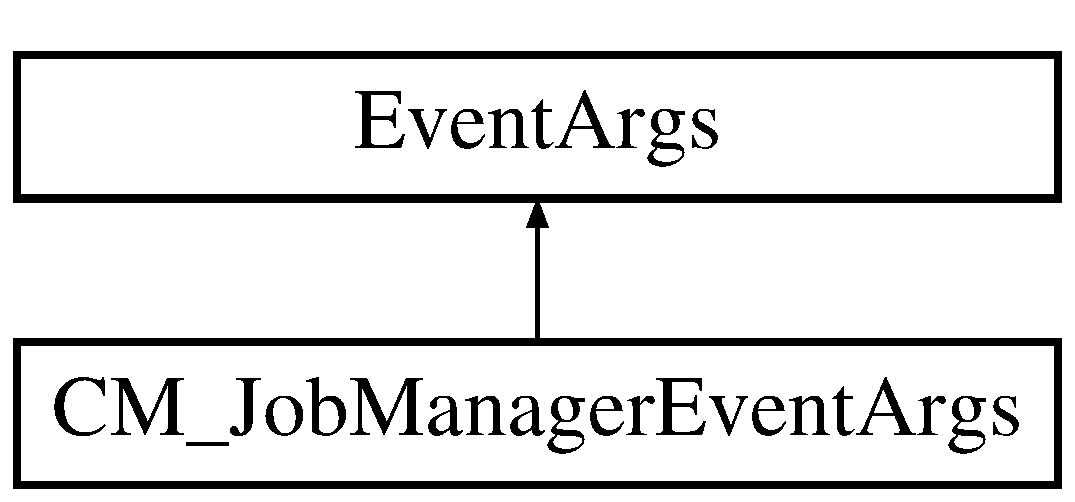
\includegraphics[height=2.000000cm]{class_c_m___job_manager_event_args}
\end{center}
\end{figure}
\subsection*{Public Member Functions}
\begin{DoxyCompactItemize}
\item 
\hyperlink{class_c_m___job_manager_event_args_a3bf019737d565f11c527b36e39dff77d}{C\+M\+\_\+\+Job\+Manager\+Event\+Args} (Dictionary$<$ string, \hyperlink{class_c_m___job}{C\+M\+\_\+\+Job} $>$ \hyperlink{class_c_m___job_manager_event_args_ab3f9e101be895139ac984b0a5abe5c55}{owned\+Jobs})
\begin{DoxyCompactList}\small\item\em Initializes a new instance of the \hyperlink{class_c_m___job_manager_event_args}{C\+M\+\_\+\+Job\+Manager\+Event\+Args} class. \end{DoxyCompactList}\end{DoxyCompactItemize}
\subsection*{Properties}
\begin{DoxyCompactItemize}
\item 
\hyperlink{class_c_m___job}{C\+M\+\_\+\+Job}\mbox{[}$\,$\mbox{]} \hyperlink{class_c_m___job_manager_event_args_ab3f9e101be895139ac984b0a5abe5c55}{owned\+Jobs}\hspace{0.3cm}{\ttfamily  \mbox{[}get\mbox{]}}
\begin{DoxyCompactList}\small\item\em Gets the owned jobs of the job manager at the time of the event being raised. \end{DoxyCompactList}\item 
\hyperlink{class_c_m___job}{C\+M\+\_\+\+Job}\mbox{[}$\,$\mbox{]} \hyperlink{class_c_m___job_manager_event_args_a354cda77d3151fa14c5a862de00c6fda}{running\+Jobs}\hspace{0.3cm}{\ttfamily  \mbox{[}get\mbox{]}}
\begin{DoxyCompactList}\small\item\em Gets the currently running jobs of the job manager at the time of the event being raised. \end{DoxyCompactList}\item 
\hyperlink{class_c_m___job}{C\+M\+\_\+\+Job}\mbox{[}$\,$\mbox{]} \hyperlink{class_c_m___job_manager_event_args_a655cd7e19559fa5cad8a10c8a4c40992}{paused\+Jobs}\hspace{0.3cm}{\ttfamily  \mbox{[}get\mbox{]}}
\begin{DoxyCompactList}\small\item\em Gets the paused jobs of the job manager at the time of the event being raised. \end{DoxyCompactList}\end{DoxyCompactItemize}


\subsection{Detailed Description}
Arguements used in events raised by \hyperlink{class_c_m___job_manager}{C\+M\+\_\+\+Job\+Manager}. 



\subsection{Constructor \& Destructor Documentation}
\hypertarget{class_c_m___job_manager_event_args_a3bf019737d565f11c527b36e39dff77d}{}\index{C\+M\+\_\+\+Job\+Manager\+Event\+Args@{C\+M\+\_\+\+Job\+Manager\+Event\+Args}!C\+M\+\_\+\+Job\+Manager\+Event\+Args@{C\+M\+\_\+\+Job\+Manager\+Event\+Args}}
\index{C\+M\+\_\+\+Job\+Manager\+Event\+Args@{C\+M\+\_\+\+Job\+Manager\+Event\+Args}!C\+M\+\_\+\+Job\+Manager\+Event\+Args@{C\+M\+\_\+\+Job\+Manager\+Event\+Args}}
\subsubsection[{C\+M\+\_\+\+Job\+Manager\+Event\+Args(\+Dictionary$<$ string, C\+M\+\_\+\+Job $>$ owned\+Jobs)}]{\setlength{\rightskip}{0pt plus 5cm}C\+M\+\_\+\+Job\+Manager\+Event\+Args.\+C\+M\+\_\+\+Job\+Manager\+Event\+Args (
\begin{DoxyParamCaption}
\item[{Dictionary$<$ string, {\bf C\+M\+\_\+\+Job} $>$}]{owned\+Jobs}
\end{DoxyParamCaption}
)}\label{class_c_m___job_manager_event_args_a3bf019737d565f11c527b36e39dff77d}


Initializes a new instance of the \hyperlink{class_c_m___job_manager_event_args}{C\+M\+\_\+\+Job\+Manager\+Event\+Args} class. 


\begin{DoxyParams}{Parameters}
{\em owned\+Jobs} & Owned jobs.\\
\hline
\end{DoxyParams}


\subsection{Property Documentation}
\hypertarget{class_c_m___job_manager_event_args_ab3f9e101be895139ac984b0a5abe5c55}{}\index{C\+M\+\_\+\+Job\+Manager\+Event\+Args@{C\+M\+\_\+\+Job\+Manager\+Event\+Args}!owned\+Jobs@{owned\+Jobs}}
\index{owned\+Jobs@{owned\+Jobs}!C\+M\+\_\+\+Job\+Manager\+Event\+Args@{C\+M\+\_\+\+Job\+Manager\+Event\+Args}}
\subsubsection[{owned\+Jobs}]{\setlength{\rightskip}{0pt plus 5cm}{\bf C\+M\+\_\+\+Job} \mbox{[}$\,$\mbox{]} C\+M\+\_\+\+Job\+Manager\+Event\+Args.\+owned\+Jobs\hspace{0.3cm}{\ttfamily [get]}}\label{class_c_m___job_manager_event_args_ab3f9e101be895139ac984b0a5abe5c55}


Gets the owned jobs of the job manager at the time of the event being raised. 

The owned jobs.\hypertarget{class_c_m___job_manager_event_args_a655cd7e19559fa5cad8a10c8a4c40992}{}\index{C\+M\+\_\+\+Job\+Manager\+Event\+Args@{C\+M\+\_\+\+Job\+Manager\+Event\+Args}!paused\+Jobs@{paused\+Jobs}}
\index{paused\+Jobs@{paused\+Jobs}!C\+M\+\_\+\+Job\+Manager\+Event\+Args@{C\+M\+\_\+\+Job\+Manager\+Event\+Args}}
\subsubsection[{paused\+Jobs}]{\setlength{\rightskip}{0pt plus 5cm}{\bf C\+M\+\_\+\+Job} \mbox{[}$\,$\mbox{]} C\+M\+\_\+\+Job\+Manager\+Event\+Args.\+paused\+Jobs\hspace{0.3cm}{\ttfamily [get]}}\label{class_c_m___job_manager_event_args_a655cd7e19559fa5cad8a10c8a4c40992}


Gets the paused jobs of the job manager at the time of the event being raised. 

The paused jobs.\hypertarget{class_c_m___job_manager_event_args_a354cda77d3151fa14c5a862de00c6fda}{}\index{C\+M\+\_\+\+Job\+Manager\+Event\+Args@{C\+M\+\_\+\+Job\+Manager\+Event\+Args}!running\+Jobs@{running\+Jobs}}
\index{running\+Jobs@{running\+Jobs}!C\+M\+\_\+\+Job\+Manager\+Event\+Args@{C\+M\+\_\+\+Job\+Manager\+Event\+Args}}
\subsubsection[{running\+Jobs}]{\setlength{\rightskip}{0pt plus 5cm}{\bf C\+M\+\_\+\+Job} \mbox{[}$\,$\mbox{]} C\+M\+\_\+\+Job\+Manager\+Event\+Args.\+running\+Jobs\hspace{0.3cm}{\ttfamily [get]}}\label{class_c_m___job_manager_event_args_a354cda77d3151fa14c5a862de00c6fda}


Gets the currently running jobs of the job manager at the time of the event being raised. 

The running jobs.

The documentation for this class was generated from the following file\+:\begin{DoxyCompactItemize}
\item 
C\+M\+\_\+\+Job\+Manager\+Event\+Args.\+cs\end{DoxyCompactItemize}

\hypertarget{class_c_m___job_manager_job_edited_event_args}{}\section{C\+M\+\_\+\+Job\+Manager\+Job\+Edited\+Event\+Args Class Reference}
\label{class_c_m___job_manager_job_edited_event_args}\index{C\+M\+\_\+\+Job\+Manager\+Job\+Edited\+Event\+Args@{C\+M\+\_\+\+Job\+Manager\+Job\+Edited\+Event\+Args}}


Arguements used in events raised by \hyperlink{class_c_m___job_manager}{C\+M\+\_\+\+Job\+Manager}.  


Inheritance diagram for C\+M\+\_\+\+Job\+Manager\+Job\+Edited\+Event\+Args\+:\begin{figure}[H]
\begin{center}
\leavevmode
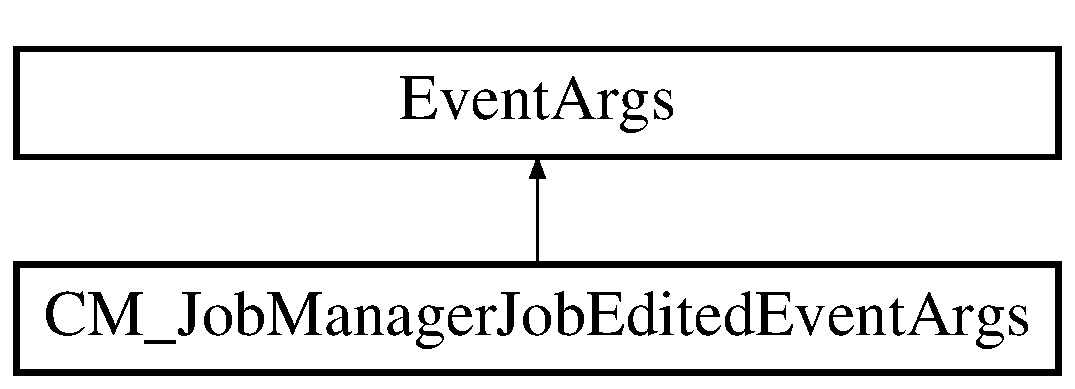
\includegraphics[height=2.000000cm]{class_c_m___job_manager_job_edited_event_args}
\end{center}
\end{figure}
\subsection*{Public Member Functions}
\begin{DoxyCompactItemize}
\item 
\hyperlink{class_c_m___job_manager_job_edited_event_args_a4affe52499a44d68c7c0cae61177583f}{C\+M\+\_\+\+Job\+Manager\+Job\+Edited\+Event\+Args} (Dictionary$<$ string, \hyperlink{class_c_m___job}{C\+M\+\_\+\+Job} $>$ owned\+Jobs, \hyperlink{class_c_m___job}{C\+M\+\_\+\+Job} \hyperlink{class_c_m___job_manager_job_edited_event_args_a7ffe2e303d15476afa5fc9d693367a8e}{job\+Edited})
\begin{DoxyCompactList}\small\item\em Initializes a new instance of the \hyperlink{class_c_m___job_manager_job_edited_event_args}{C\+M\+\_\+\+Job\+Manager\+Job\+Edited\+Event\+Args} class. \end{DoxyCompactList}\end{DoxyCompactItemize}
\subsection*{Properties}
\begin{DoxyCompactItemize}
\item 
\hyperlink{class_c_m___job_manager_event_args}{C\+M\+\_\+\+Job\+Manager\+Event\+Args} \hyperlink{class_c_m___job_manager_job_edited_event_args_a5baf47bf8ecddf8a6f88b0779a504670}{other\+Args}\hspace{0.3cm}{\ttfamily  \mbox{[}get\mbox{]}}
\begin{DoxyCompactList}\small\item\em Gets the other arguments. \end{DoxyCompactList}\item 
\hyperlink{class_c_m___job}{C\+M\+\_\+\+Job} \hyperlink{class_c_m___job_manager_job_edited_event_args_a7ffe2e303d15476afa5fc9d693367a8e}{job\+Edited}\hspace{0.3cm}{\ttfamily  \mbox{[}get\mbox{]}}
\begin{DoxyCompactList}\small\item\em Gets the job currently changed that caused the event to be raised. \end{DoxyCompactList}\end{DoxyCompactItemize}


\subsection{Detailed Description}
Arguements used in events raised by \hyperlink{class_c_m___job_manager}{C\+M\+\_\+\+Job\+Manager}. 



\subsection{Constructor \& Destructor Documentation}
\hypertarget{class_c_m___job_manager_job_edited_event_args_a4affe52499a44d68c7c0cae61177583f}{}\index{C\+M\+\_\+\+Job\+Manager\+Job\+Edited\+Event\+Args@{C\+M\+\_\+\+Job\+Manager\+Job\+Edited\+Event\+Args}!C\+M\+\_\+\+Job\+Manager\+Job\+Edited\+Event\+Args@{C\+M\+\_\+\+Job\+Manager\+Job\+Edited\+Event\+Args}}
\index{C\+M\+\_\+\+Job\+Manager\+Job\+Edited\+Event\+Args@{C\+M\+\_\+\+Job\+Manager\+Job\+Edited\+Event\+Args}!C\+M\+\_\+\+Job\+Manager\+Job\+Edited\+Event\+Args@{C\+M\+\_\+\+Job\+Manager\+Job\+Edited\+Event\+Args}}
\subsubsection[{C\+M\+\_\+\+Job\+Manager\+Job\+Edited\+Event\+Args(\+Dictionary$<$ string, C\+M\+\_\+\+Job $>$ owned\+Jobs, C\+M\+\_\+\+Job job\+Edited)}]{\setlength{\rightskip}{0pt plus 5cm}C\+M\+\_\+\+Job\+Manager\+Job\+Edited\+Event\+Args.\+C\+M\+\_\+\+Job\+Manager\+Job\+Edited\+Event\+Args (
\begin{DoxyParamCaption}
\item[{Dictionary$<$ string, {\bf C\+M\+\_\+\+Job} $>$}]{owned\+Jobs, }
\item[{{\bf C\+M\+\_\+\+Job}}]{job\+Edited}
\end{DoxyParamCaption}
)}\label{class_c_m___job_manager_job_edited_event_args_a4affe52499a44d68c7c0cae61177583f}


Initializes a new instance of the \hyperlink{class_c_m___job_manager_job_edited_event_args}{C\+M\+\_\+\+Job\+Manager\+Job\+Edited\+Event\+Args} class. 


\begin{DoxyParams}{Parameters}
{\em owned\+Jobs} & Owned jobs.\\
\hline
{\em job\+Edited} & Job edited.\\
\hline
\end{DoxyParams}


\subsection{Property Documentation}
\hypertarget{class_c_m___job_manager_job_edited_event_args_a7ffe2e303d15476afa5fc9d693367a8e}{}\index{C\+M\+\_\+\+Job\+Manager\+Job\+Edited\+Event\+Args@{C\+M\+\_\+\+Job\+Manager\+Job\+Edited\+Event\+Args}!job\+Edited@{job\+Edited}}
\index{job\+Edited@{job\+Edited}!C\+M\+\_\+\+Job\+Manager\+Job\+Edited\+Event\+Args@{C\+M\+\_\+\+Job\+Manager\+Job\+Edited\+Event\+Args}}
\subsubsection[{job\+Edited}]{\setlength{\rightskip}{0pt plus 5cm}{\bf C\+M\+\_\+\+Job} C\+M\+\_\+\+Job\+Manager\+Job\+Edited\+Event\+Args.\+job\+Edited\hspace{0.3cm}{\ttfamily [get]}}\label{class_c_m___job_manager_job_edited_event_args_a7ffe2e303d15476afa5fc9d693367a8e}


Gets the job currently changed that caused the event to be raised. 

The job edited.\hypertarget{class_c_m___job_manager_job_edited_event_args_a5baf47bf8ecddf8a6f88b0779a504670}{}\index{C\+M\+\_\+\+Job\+Manager\+Job\+Edited\+Event\+Args@{C\+M\+\_\+\+Job\+Manager\+Job\+Edited\+Event\+Args}!other\+Args@{other\+Args}}
\index{other\+Args@{other\+Args}!C\+M\+\_\+\+Job\+Manager\+Job\+Edited\+Event\+Args@{C\+M\+\_\+\+Job\+Manager\+Job\+Edited\+Event\+Args}}
\subsubsection[{other\+Args}]{\setlength{\rightskip}{0pt plus 5cm}{\bf C\+M\+\_\+\+Job\+Manager\+Event\+Args} C\+M\+\_\+\+Job\+Manager\+Job\+Edited\+Event\+Args.\+other\+Args\hspace{0.3cm}{\ttfamily [get]}}\label{class_c_m___job_manager_job_edited_event_args_a5baf47bf8ecddf8a6f88b0779a504670}


Gets the other arguments. 

The other arguments.

The documentation for this class was generated from the following file\+:\begin{DoxyCompactItemize}
\item 
C\+M\+\_\+\+Job\+Manager\+Job\+Edited\+Event\+Args.\+cs\end{DoxyCompactItemize}

\hypertarget{class_c_m___job_queue}{}\section{C\+M\+\_\+\+Job\+Queue Class Reference}
\label{class_c_m___job_queue}\index{C\+M\+\_\+\+Job\+Queue@{C\+M\+\_\+\+Job\+Queue}}


The main job queue class. Encapsulates all behaviour related to queueing a job. Provides access to events, and status (i.\+e. running, repeating).  


Inheritance diagram for C\+M\+\_\+\+Job\+Queue\+:\begin{figure}[H]
\begin{center}
\leavevmode
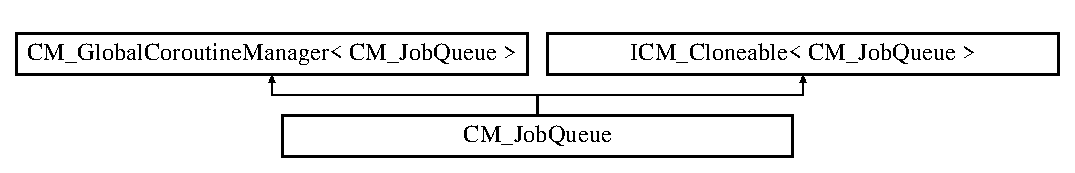
\includegraphics[height=1.872910cm]{class_c_m___job_queue}
\end{center}
\end{figure}
\subsection*{Public Member Functions}
\begin{DoxyCompactItemize}
\item 
\hyperlink{class_c_m___job_queue}{C\+M\+\_\+\+Job\+Queue} \hyperlink{class_c_m___job_queue_a32411811468c3df358fa1b1dd20da0e9}{Clone} ()
\begin{DoxyCompactList}\small\item\em Clone this instance. \end{DoxyCompactList}\item 
\hyperlink{class_c_m___job_queue}{C\+M\+\_\+\+Job\+Queue}\mbox{[}$\,$\mbox{]} \hyperlink{class_c_m___job_queue_ab9d4d607c63d9099694bbefcf46b0651}{Clone} (int num\+Of\+Copies)
\begin{DoxyCompactList}\small\item\em Clone this instance the specified num\+Of\+Copies. \end{DoxyCompactList}\item 
\hyperlink{class_c_m___job_queue}{C\+M\+\_\+\+Job\+Queue} \hyperlink{class_c_m___job_queue_a5eb3ac10485cd8620f53d38eb413a53d}{Enqueue} (\hyperlink{class_c_m___job_queue}{C\+M\+\_\+\+Job\+Queue} other)
\begin{DoxyCompactList}\small\item\em Enqueues the specified other queue. Adds the jobs from one queue to this queue and also adds the other queues event subscriptions. \end{DoxyCompactList}\item 
\hyperlink{class_c_m___job_queue}{C\+M\+\_\+\+Job\+Queue} \hyperlink{class_c_m___job_queue_a8d85bdcd2a9db1085837622ca6f39fb2}{Enqueue} (params \hyperlink{class_c_m___job}{C\+M\+\_\+\+Job}\mbox{[}$\,$\mbox{]} jobs)
\begin{DoxyCompactList}\small\item\em Enqueues the specified jobs. \end{DoxyCompactList}\item 
\hyperlink{class_c_m___job_queue}{C\+M\+\_\+\+Job\+Queue} \hyperlink{class_c_m___job_queue_a03261e561d34769b869c8f054e7c90d4}{Enqueue} (I\+List$<$ \hyperlink{class_c_m___job}{C\+M\+\_\+\+Job} $>$ jobs)
\begin{DoxyCompactList}\small\item\em Enqueues the specified jobs. \end{DoxyCompactList}\item 
\hyperlink{class_c_m___job_queue}{C\+M\+\_\+\+Job\+Queue} \hyperlink{class_c_m___job_queue_a8c3f4534e75a50c47a64d3324ca75f67}{Enqueue} (string id, I\+Enumerator routine)
\begin{DoxyCompactList}\small\item\em Creates a new job with specified id and coroutine and adds job to queue. \end{DoxyCompactList}\item 
\hyperlink{class_c_m___job_queue}{C\+M\+\_\+\+Job\+Queue} \hyperlink{class_c_m___job_queue_a36897e683ccf438e4f1e032645423cd5}{Enqueue} (I\+Enumerator routine)
\begin{DoxyCompactList}\small\item\em Creates a new job with specified id and coroutine and adds job to queue. \end{DoxyCompactList}\item 
\hyperlink{class_c_m___job_queue}{C\+M\+\_\+\+Job\+Queue} \hyperlink{class_c_m___job_queue_a5a0c5479c91848563c3dbc0e4c218f14}{Enqueue} (\hyperlink{class_c_m___job}{C\+M\+\_\+\+Job} job)
\begin{DoxyCompactList}\small\item\em Enqueues the specified job. \end{DoxyCompactList}\item 
\hyperlink{class_c_m___job_queue}{C\+M\+\_\+\+Job\+Queue} \hyperlink{class_c_m___job_queue_a0b741b6ee48616f0bc2f1e14360f0575}{Start} ()
\begin{DoxyCompactList}\small\item\em Start this instance of the queue immediately. \end{DoxyCompactList}\item 
\hyperlink{class_c_m___job_queue}{C\+M\+\_\+\+Job\+Queue} \hyperlink{class_c_m___job_queue_afacbda3a733d0a18f0791923ffcbb4fa}{Start} (float delay\+In\+Seconds)
\begin{DoxyCompactList}\small\item\em Start the specified instance after delay\+In\+Seconds. \end{DoxyCompactList}\item 
\hyperlink{class_c_m___job_queue}{C\+M\+\_\+\+Job\+Queue} \hyperlink{class_c_m___job_queue_acf86ac86cf4899aa34e1951f657ff66a}{Repeat} ()
\begin{DoxyCompactList}\small\item\em Sets this instance to repeat. The job is repeated when it has finished processing. \end{DoxyCompactList}\item 
\hyperlink{class_c_m___job_queue}{C\+M\+\_\+\+Job\+Queue} \hyperlink{class_c_m___job_queue_a26edb6cc573aed7c1804b7a6dae1d450}{Repeat} (int num\+Of\+Times)
\begin{DoxyCompactList}\small\item\em Sets this instance to repeat a number of times. The job is repeated when it has finished processing. \end{DoxyCompactList}\item 
\hyperlink{class_c_m___job_queue}{C\+M\+\_\+\+Job\+Queue} \hyperlink{class_c_m___job_queue_a4b9474030edaa4b85e120774858b2050}{Stop\+Repeat} ()
\begin{DoxyCompactList}\small\item\em Stops the repeat. \end{DoxyCompactList}\item 
\hyperlink{class_c_m___job_queue}{C\+M\+\_\+\+Job\+Queue} \hyperlink{class_c_m___job_queue_a863d01fa168f36f665787bb2b1a8be1c}{Stop\+Repeat} (float delay\+In\+Seconds)
\begin{DoxyCompactList}\small\item\em Stops the repeat after a specified delay in seconds. \end{DoxyCompactList}\item 
\hyperlink{class_c_m___job_queue}{C\+M\+\_\+\+Job\+Queue} \hyperlink{class_c_m___job_queue_a40d741107627777352ebd2e0478f3955}{Pause} ()
\begin{DoxyCompactList}\small\item\em Pauses this instance. \end{DoxyCompactList}\item 
\hyperlink{class_c_m___job_queue}{C\+M\+\_\+\+Job\+Queue} \hyperlink{class_c_m___job_queue_a705adde1f43487cf5b78599e09c85180}{Pause} (float delay\+In\+Seconds)
\begin{DoxyCompactList}\small\item\em Pause this instance after the specified delay\+In\+Seconds. \end{DoxyCompactList}\item 
\hyperlink{class_c_m___job_queue}{C\+M\+\_\+\+Job\+Queue} \hyperlink{class_c_m___job_queue_a6d3357eaff31b561a0db4de7e14e937b}{Resume} ()
\begin{DoxyCompactList}\small\item\em Resume this instance immediately. \end{DoxyCompactList}\item 
\hyperlink{class_c_m___job_queue}{C\+M\+\_\+\+Job\+Queue} \hyperlink{class_c_m___job_queue_a4d7818132595a2a97b9350f810405c1c}{Resume} (float delay\+In\+Seconds)
\begin{DoxyCompactList}\small\item\em Resume the instance after the specified delay\+In\+Seconds. \end{DoxyCompactList}\item 
\hyperlink{class_c_m___job_queue}{C\+M\+\_\+\+Job\+Queue} \hyperlink{class_c_m___job_queue_a8b0a472fcdce0ddba4576bfe39feb7ff}{Continous\+Running} ()
\begin{DoxyCompactList}\small\item\em Set the queue to run continously. \end{DoxyCompactList}\item 
\hyperlink{class_c_m___job_queue}{C\+M\+\_\+\+Job\+Queue} \hyperlink{class_c_m___job_queue_a636825476d970cc13724f73ae9e288ee}{Stop\+Continous\+Running} ()
\begin{DoxyCompactList}\small\item\em Stops the continous running of this queue. \end{DoxyCompactList}\item 
\hyperlink{class_c_m___job_queue}{C\+M\+\_\+\+Job\+Queue} \hyperlink{class_c_m___job_queue_a194f2954b520d2984ff313d3c675dce2}{Kill\+All} ()
\begin{DoxyCompactList}\small\item\em Kill all currently queued jobs immediately. Clears queue list. \end{DoxyCompactList}\item 
\hyperlink{class_c_m___job_queue}{C\+M\+\_\+\+Job\+Queue} \hyperlink{class_c_m___job_queue_adce8edbf35e9f320611f789262d215c6}{Kill\+All} (float delay\+In\+Seconds)
\begin{DoxyCompactList}\small\item\em Kill all currently queued jobs after the specified delay\+In\+Seconds. \end{DoxyCompactList}\item 
\hyperlink{class_c_m___job_queue}{C\+M\+\_\+\+Job\+Queue} \hyperlink{class_c_m___job_queue_aeb73327ca071773270823880e4ce9f31}{Kill\+Current} ()
\begin{DoxyCompactList}\small\item\em Kills the current running job immediately. \end{DoxyCompactList}\item 
\hyperlink{class_c_m___job_queue}{C\+M\+\_\+\+Job\+Queue} \hyperlink{class_c_m___job_queue_ac3cb68f5d7fb1f63d95cf8ac8eff0172}{Kill\+Current} (float delay\+In\+Seconds)
\begin{DoxyCompactList}\small\item\em Kills the current running job after the specified delay\+In\+Seconds. \end{DoxyCompactList}\item 
\hyperlink{class_c_m___job_queue}{C\+M\+\_\+\+Job\+Queue} \hyperlink{class_c_m___job_queue_a2918eb628f865860a22032eafa3618b5}{Notify\+On\+Queue\+Started} (Event\+Handler$<$ \hyperlink{class_c_m___queue_event_args}{C\+M\+\_\+\+Queue\+Event\+Args} $>$ e)
\begin{DoxyCompactList}\small\item\em Subscribes to the queue started event. \end{DoxyCompactList}\item 
\hyperlink{class_c_m___job_queue}{C\+M\+\_\+\+Job\+Queue} \hyperlink{class_c_m___job_queue_a772043be6d95571dffe266eefb99a99f}{Remove\+Notify\+On\+Queue\+Started} (Event\+Handler$<$ \hyperlink{class_c_m___queue_event_args}{C\+M\+\_\+\+Queue\+Event\+Args} $>$ e)
\begin{DoxyCompactList}\small\item\em Unsubscribes to the the queue started event. \end{DoxyCompactList}\item 
\hyperlink{class_c_m___job_queue}{C\+M\+\_\+\+Job\+Queue} \hyperlink{class_c_m___job_queue_af9aec1172b9818353bae58cb013b445d}{Notify\+On\+Queue\+Complete} (Event\+Handler$<$ \hyperlink{class_c_m___queue_event_args}{C\+M\+\_\+\+Queue\+Event\+Args} $>$ e)
\begin{DoxyCompactList}\small\item\em Subscribes to the queue completed event. \end{DoxyCompactList}\item 
\hyperlink{class_c_m___job_queue}{C\+M\+\_\+\+Job\+Queue} \hyperlink{class_c_m___job_queue_a77456f4bd081c75ba385f96e1d72077a}{Remove\+Notify\+On\+Queue\+Complete} (Event\+Handler$<$ \hyperlink{class_c_m___queue_event_args}{C\+M\+\_\+\+Queue\+Event\+Args} $>$ e)
\begin{DoxyCompactList}\small\item\em Unsubscribes to the queue completed event. \end{DoxyCompactList}\item 
\hyperlink{class_c_m___job_queue}{C\+M\+\_\+\+Job\+Queue} \hyperlink{class_c_m___job_queue_a6e17336d22c1588d5836d1053749467e}{Notify\+On\+Job\+Processed} (Event\+Handler$<$ \hyperlink{class_c_m___queue_event_args}{C\+M\+\_\+\+Queue\+Event\+Args} $>$ e)
\begin{DoxyCompactList}\small\item\em Subscribes to the the job processed event. \end{DoxyCompactList}\item 
\hyperlink{class_c_m___job_queue}{C\+M\+\_\+\+Job\+Queue} \hyperlink{class_c_m___job_queue_aa947d55c737bee485b24a621a3780046}{Remove\+Notify\+On\+Job\+Processed} (Event\+Handler$<$ \hyperlink{class_c_m___queue_event_args}{C\+M\+\_\+\+Queue\+Event\+Args} $>$ e)
\begin{DoxyCompactList}\small\item\em Unsubscribes to the the job processed event. This event is invoked every time a job in the queue has finished running. \end{DoxyCompactList}\end{DoxyCompactItemize}
\subsection*{Static Public Member Functions}
\begin{DoxyCompactItemize}
\item 
static \hyperlink{class_c_m___job_queue}{C\+M\+\_\+\+Job\+Queue} \hyperlink{class_c_m___job_queue_ab9832aba052e19ef3c726a05ca4849fa}{Make} ()
\begin{DoxyCompactList}\small\item\em Returns an initialised \hyperlink{class_c_m___job_queue}{C\+M\+\_\+\+Job\+Queue} instance. Provides static access to class. \end{DoxyCompactList}\end{DoxyCompactItemize}
\subsection*{Protected Member Functions}
\begin{DoxyCompactItemize}
\item 
void \hyperlink{class_c_m___job_queue_a3f9c1e210a1fb9d64459d50620548656}{On\+Queue\+Started} (\hyperlink{class_c_m___queue_event_args}{C\+M\+\_\+\+Queue\+Event\+Args} e)
\begin{DoxyCompactList}\small\item\em Raises the queue started event. \end{DoxyCompactList}\item 
void \hyperlink{class_c_m___job_queue_adc533901dffcd84b9e507e2dc848a414}{On\+Queue\+Complete} (\hyperlink{class_c_m___queue_event_args}{C\+M\+\_\+\+Queue\+Event\+Args} e)
\begin{DoxyCompactList}\small\item\em Raises the queue complete event. \end{DoxyCompactList}\item 
void \hyperlink{class_c_m___job_queue_a50f9608ca896727a3e993b2015a790a6}{On\+Job\+Processed} (\hyperlink{class_c_m___queue_event_args}{C\+M\+\_\+\+Queue\+Event\+Args} e)
\begin{DoxyCompactList}\small\item\em Raises the job processed event. \end{DoxyCompactList}\item 
override void \hyperlink{class_c_m___job_queue_afa8b77f601ce5094b44ad694d23e54f4}{Handlejob\+Complete} (object sender, \hyperlink{class_c_m___job_event_args}{C\+M\+\_\+\+Job\+Event\+Args} e)
\begin{DoxyCompactList}\small\item\em Invoked whenever a queued job has finished processing. Handles maintenance of queue and raising On\+Job\+Processed and On\+Queue\+Complete events. \end{DoxyCompactList}\end{DoxyCompactItemize}
\subsection*{Properties}
\begin{DoxyCompactItemize}
\item 
bool \hyperlink{class_c_m___job_queue_a652f13e97ccd6cd66fe899e0d4612842}{repeating}\hspace{0.3cm}{\ttfamily  \mbox{[}get\mbox{]}}
\begin{DoxyCompactList}\small\item\em Gets a value indicating whether this \hyperlink{class_c_m___job_queue}{C\+M\+\_\+\+Job\+Queue} is repeating. \end{DoxyCompactList}\item 
int \hyperlink{class_c_m___job_queue_a09c449c39674203848e7d939e3742460}{num\+Of\+Times\+Executed}\hspace{0.3cm}{\ttfamily  \mbox{[}get\mbox{]}}
\begin{DoxyCompactList}\small\item\em Gets the number of times this queue executed (used if repeating). \end{DoxyCompactList}\item 
bool \hyperlink{class_c_m___job_queue_aa7e3982beb8c64bf115c0adc30134d84}{running}\hspace{0.3cm}{\ttfamily  \mbox{[}get\mbox{]}}
\begin{DoxyCompactList}\small\item\em Gets a value indicating whether this \hyperlink{class_c_m___job_queue}{C\+M\+\_\+\+Job\+Queue} is running. \end{DoxyCompactList}\item 
bool \hyperlink{class_c_m___job_queue_a93ffe57018263669329b70e523ac8fa1}{continous\+Running}\hspace{0.3cm}{\ttfamily  \mbox{[}get\mbox{]}}
\begin{DoxyCompactList}\small\item\em Gets a value indicating whether this \hyperlink{class_c_m___job_queue}{C\+M\+\_\+\+Job\+Queue} is running continously i.\+e. will not stop running until Stop\+Continous\+Running is called. \end{DoxyCompactList}\end{DoxyCompactItemize}
\subsection*{Events}
\begin{DoxyCompactItemize}
\item 
Event\+Handler$<$ \hyperlink{class_c_m___queue_event_args}{C\+M\+\_\+\+Queue\+Event\+Args} $>$ \hyperlink{class_c_m___job_queue_a758ae5902e82e8690264d2f7a61f9ae0}{queue\+Started}
\begin{DoxyCompactList}\small\item\em Raised when queue started. \end{DoxyCompactList}\item 
Event\+Handler$<$ \hyperlink{class_c_m___queue_event_args}{C\+M\+\_\+\+Queue\+Event\+Args} $>$ \hyperlink{class_c_m___job_queue_a66eb2a7f16850398ae06ddf02372f64e}{queue\+Complete}
\begin{DoxyCompactList}\small\item\em Raised when queue complete. \end{DoxyCompactList}\item 
Event\+Handler$<$ \hyperlink{class_c_m___queue_event_args}{C\+M\+\_\+\+Queue\+Event\+Args} $>$ \hyperlink{class_c_m___job_queue_a331d3a29f310ac03de1e631e6af67404}{job\+Processed}
\begin{DoxyCompactList}\small\item\em Raised when a job in the queue has finished. \end{DoxyCompactList}\end{DoxyCompactItemize}


\subsection{Detailed Description}
The main job queue class. Encapsulates all behaviour related to queueing a job. Provides access to events, and status (i.\+e. running, repeating). 



\subsection{Member Function Documentation}
\hypertarget{class_c_m___job_queue_a32411811468c3df358fa1b1dd20da0e9}{}\index{C\+M\+\_\+\+Job\+Queue@{C\+M\+\_\+\+Job\+Queue}!Clone@{Clone}}
\index{Clone@{Clone}!C\+M\+\_\+\+Job\+Queue@{C\+M\+\_\+\+Job\+Queue}}
\subsubsection[{Clone()}]{\setlength{\rightskip}{0pt plus 5cm}{\bf C\+M\+\_\+\+Job\+Queue} C\+M\+\_\+\+Job\+Queue.\+Clone (
\begin{DoxyParamCaption}
{}
\end{DoxyParamCaption}
)}\label{class_c_m___job_queue_a32411811468c3df358fa1b1dd20da0e9}


Clone this instance. 

\hypertarget{class_c_m___job_queue_ab9d4d607c63d9099694bbefcf46b0651}{}\index{C\+M\+\_\+\+Job\+Queue@{C\+M\+\_\+\+Job\+Queue}!Clone@{Clone}}
\index{Clone@{Clone}!C\+M\+\_\+\+Job\+Queue@{C\+M\+\_\+\+Job\+Queue}}
\subsubsection[{Clone(int num\+Of\+Copies)}]{\setlength{\rightskip}{0pt plus 5cm}{\bf C\+M\+\_\+\+Job\+Queue} \mbox{[}$\,$\mbox{]} C\+M\+\_\+\+Job\+Queue.\+Clone (
\begin{DoxyParamCaption}
\item[{int}]{num\+Of\+Copies}
\end{DoxyParamCaption}
)}\label{class_c_m___job_queue_ab9d4d607c63d9099694bbefcf46b0651}


Clone this instance the specified num\+Of\+Copies. 


\begin{DoxyParams}{Parameters}
{\em num\+Of\+Copies} & Number of copies.\\
\hline
\end{DoxyParams}
\hypertarget{class_c_m___job_queue_a8b0a472fcdce0ddba4576bfe39feb7ff}{}\index{C\+M\+\_\+\+Job\+Queue@{C\+M\+\_\+\+Job\+Queue}!Continous\+Running@{Continous\+Running}}
\index{Continous\+Running@{Continous\+Running}!C\+M\+\_\+\+Job\+Queue@{C\+M\+\_\+\+Job\+Queue}}
\subsubsection[{Continous\+Running()}]{\setlength{\rightskip}{0pt plus 5cm}{\bf C\+M\+\_\+\+Job\+Queue} C\+M\+\_\+\+Job\+Queue.\+Continous\+Running (
\begin{DoxyParamCaption}
{}
\end{DoxyParamCaption}
)}\label{class_c_m___job_queue_a8b0a472fcdce0ddba4576bfe39feb7ff}


Set the queue to run continously. 

\hypertarget{class_c_m___job_queue_a5eb3ac10485cd8620f53d38eb413a53d}{}\index{C\+M\+\_\+\+Job\+Queue@{C\+M\+\_\+\+Job\+Queue}!Enqueue@{Enqueue}}
\index{Enqueue@{Enqueue}!C\+M\+\_\+\+Job\+Queue@{C\+M\+\_\+\+Job\+Queue}}
\subsubsection[{Enqueue(\+C\+M\+\_\+\+Job\+Queue other)}]{\setlength{\rightskip}{0pt plus 5cm}{\bf C\+M\+\_\+\+Job\+Queue} C\+M\+\_\+\+Job\+Queue.\+Enqueue (
\begin{DoxyParamCaption}
\item[{{\bf C\+M\+\_\+\+Job\+Queue}}]{other}
\end{DoxyParamCaption}
)}\label{class_c_m___job_queue_a5eb3ac10485cd8620f53d38eb413a53d}


Enqueues the specified other queue. Adds the jobs from one queue to this queue and also adds the other queues event subscriptions. 


\begin{DoxyParams}{Parameters}
{\em other} & Other.\\
\hline
\end{DoxyParams}
\hypertarget{class_c_m___job_queue_a8d85bdcd2a9db1085837622ca6f39fb2}{}\index{C\+M\+\_\+\+Job\+Queue@{C\+M\+\_\+\+Job\+Queue}!Enqueue@{Enqueue}}
\index{Enqueue@{Enqueue}!C\+M\+\_\+\+Job\+Queue@{C\+M\+\_\+\+Job\+Queue}}
\subsubsection[{Enqueue(params C\+M\+\_\+\+Job[] jobs)}]{\setlength{\rightskip}{0pt plus 5cm}{\bf C\+M\+\_\+\+Job\+Queue} C\+M\+\_\+\+Job\+Queue.\+Enqueue (
\begin{DoxyParamCaption}
\item[{params {\bf C\+M\+\_\+\+Job}\mbox{[}$\,$\mbox{]}}]{jobs}
\end{DoxyParamCaption}
)}\label{class_c_m___job_queue_a8d85bdcd2a9db1085837622ca6f39fb2}


Enqueues the specified jobs. 


\begin{DoxyParams}{Parameters}
{\em jobs} & Jobs.\\
\hline
\end{DoxyParams}
\hypertarget{class_c_m___job_queue_a03261e561d34769b869c8f054e7c90d4}{}\index{C\+M\+\_\+\+Job\+Queue@{C\+M\+\_\+\+Job\+Queue}!Enqueue@{Enqueue}}
\index{Enqueue@{Enqueue}!C\+M\+\_\+\+Job\+Queue@{C\+M\+\_\+\+Job\+Queue}}
\subsubsection[{Enqueue(\+I\+List$<$ C\+M\+\_\+\+Job $>$ jobs)}]{\setlength{\rightskip}{0pt plus 5cm}{\bf C\+M\+\_\+\+Job\+Queue} C\+M\+\_\+\+Job\+Queue.\+Enqueue (
\begin{DoxyParamCaption}
\item[{I\+List$<$ {\bf C\+M\+\_\+\+Job} $>$}]{jobs}
\end{DoxyParamCaption}
)}\label{class_c_m___job_queue_a03261e561d34769b869c8f054e7c90d4}


Enqueues the specified jobs. 


\begin{DoxyParams}{Parameters}
{\em jobs} & Jobs.\\
\hline
\end{DoxyParams}
\hypertarget{class_c_m___job_queue_a8c3f4534e75a50c47a64d3324ca75f67}{}\index{C\+M\+\_\+\+Job\+Queue@{C\+M\+\_\+\+Job\+Queue}!Enqueue@{Enqueue}}
\index{Enqueue@{Enqueue}!C\+M\+\_\+\+Job\+Queue@{C\+M\+\_\+\+Job\+Queue}}
\subsubsection[{Enqueue(string id, I\+Enumerator routine)}]{\setlength{\rightskip}{0pt plus 5cm}{\bf C\+M\+\_\+\+Job\+Queue} C\+M\+\_\+\+Job\+Queue.\+Enqueue (
\begin{DoxyParamCaption}
\item[{string}]{id, }
\item[{I\+Enumerator}]{routine}
\end{DoxyParamCaption}
)}\label{class_c_m___job_queue_a8c3f4534e75a50c47a64d3324ca75f67}


Creates a new job with specified id and coroutine and adds job to queue. 


\begin{DoxyParams}{Parameters}
{\em id} & Job Identifier.\\
\hline
{\em routine} & Routine.\\
\hline
\end{DoxyParams}
\hypertarget{class_c_m___job_queue_a36897e683ccf438e4f1e032645423cd5}{}\index{C\+M\+\_\+\+Job\+Queue@{C\+M\+\_\+\+Job\+Queue}!Enqueue@{Enqueue}}
\index{Enqueue@{Enqueue}!C\+M\+\_\+\+Job\+Queue@{C\+M\+\_\+\+Job\+Queue}}
\subsubsection[{Enqueue(\+I\+Enumerator routine)}]{\setlength{\rightskip}{0pt plus 5cm}{\bf C\+M\+\_\+\+Job\+Queue} C\+M\+\_\+\+Job\+Queue.\+Enqueue (
\begin{DoxyParamCaption}
\item[{I\+Enumerator}]{routine}
\end{DoxyParamCaption}
)}\label{class_c_m___job_queue_a36897e683ccf438e4f1e032645423cd5}


Creates a new job with specified id and coroutine and adds job to queue. 


\begin{DoxyParams}{Parameters}
{\em id} & Job Identifier.\\
\hline
{\em routine} & Routine.\\
\hline
\end{DoxyParams}
\hypertarget{class_c_m___job_queue_a5a0c5479c91848563c3dbc0e4c218f14}{}\index{C\+M\+\_\+\+Job\+Queue@{C\+M\+\_\+\+Job\+Queue}!Enqueue@{Enqueue}}
\index{Enqueue@{Enqueue}!C\+M\+\_\+\+Job\+Queue@{C\+M\+\_\+\+Job\+Queue}}
\subsubsection[{Enqueue(\+C\+M\+\_\+\+Job job)}]{\setlength{\rightskip}{0pt plus 5cm}{\bf C\+M\+\_\+\+Job\+Queue} C\+M\+\_\+\+Job\+Queue.\+Enqueue (
\begin{DoxyParamCaption}
\item[{{\bf C\+M\+\_\+\+Job}}]{job}
\end{DoxyParamCaption}
)}\label{class_c_m___job_queue_a5a0c5479c91848563c3dbc0e4c218f14}


Enqueues the specified job. 


\begin{DoxyParams}{Parameters}
{\em job} & Job.\\
\hline
\end{DoxyParams}
\hypertarget{class_c_m___job_queue_afa8b77f601ce5094b44ad694d23e54f4}{}\index{C\+M\+\_\+\+Job\+Queue@{C\+M\+\_\+\+Job\+Queue}!Handlejob\+Complete@{Handlejob\+Complete}}
\index{Handlejob\+Complete@{Handlejob\+Complete}!C\+M\+\_\+\+Job\+Queue@{C\+M\+\_\+\+Job\+Queue}}
\subsubsection[{Handlejob\+Complete(object sender, C\+M\+\_\+\+Job\+Event\+Args e)}]{\setlength{\rightskip}{0pt plus 5cm}override void C\+M\+\_\+\+Job\+Queue.\+Handlejob\+Complete (
\begin{DoxyParamCaption}
\item[{object}]{sender, }
\item[{{\bf C\+M\+\_\+\+Job\+Event\+Args}}]{e}
\end{DoxyParamCaption}
)\hspace{0.3cm}{\ttfamily [protected]}, {\ttfamily [virtual]}}\label{class_c_m___job_queue_afa8b77f601ce5094b44ad694d23e54f4}


Invoked whenever a queued job has finished processing. Handles maintenance of queue and raising On\+Job\+Processed and On\+Queue\+Complete events. 


\begin{DoxyParams}{Parameters}
{\em sender} & Sender.\\
\hline
{\em e} & E.\\
\hline
\end{DoxyParams}


Implements \hyperlink{class_c_m___global_coroutine_manager}{C\+M\+\_\+\+Global\+Coroutine\+Manager$<$ C\+M\+\_\+\+Job\+Queue $>$}.

\hypertarget{class_c_m___job_queue_a194f2954b520d2984ff313d3c675dce2}{}\index{C\+M\+\_\+\+Job\+Queue@{C\+M\+\_\+\+Job\+Queue}!Kill\+All@{Kill\+All}}
\index{Kill\+All@{Kill\+All}!C\+M\+\_\+\+Job\+Queue@{C\+M\+\_\+\+Job\+Queue}}
\subsubsection[{Kill\+All()}]{\setlength{\rightskip}{0pt plus 5cm}{\bf C\+M\+\_\+\+Job\+Queue} C\+M\+\_\+\+Job\+Queue.\+Kill\+All (
\begin{DoxyParamCaption}
{}
\end{DoxyParamCaption}
)}\label{class_c_m___job_queue_a194f2954b520d2984ff313d3c675dce2}


Kill all currently queued jobs immediately. Clears queue list. 

\hypertarget{class_c_m___job_queue_adce8edbf35e9f320611f789262d215c6}{}\index{C\+M\+\_\+\+Job\+Queue@{C\+M\+\_\+\+Job\+Queue}!Kill\+All@{Kill\+All}}
\index{Kill\+All@{Kill\+All}!C\+M\+\_\+\+Job\+Queue@{C\+M\+\_\+\+Job\+Queue}}
\subsubsection[{Kill\+All(float delay\+In\+Seconds)}]{\setlength{\rightskip}{0pt plus 5cm}{\bf C\+M\+\_\+\+Job\+Queue} C\+M\+\_\+\+Job\+Queue.\+Kill\+All (
\begin{DoxyParamCaption}
\item[{float}]{delay\+In\+Seconds}
\end{DoxyParamCaption}
)}\label{class_c_m___job_queue_adce8edbf35e9f320611f789262d215c6}


Kill all currently queued jobs after the specified delay\+In\+Seconds. 


\begin{DoxyParams}{Parameters}
{\em delay\+In\+Seconds} & Delay in seconds.\\
\hline
\end{DoxyParams}
\hypertarget{class_c_m___job_queue_aeb73327ca071773270823880e4ce9f31}{}\index{C\+M\+\_\+\+Job\+Queue@{C\+M\+\_\+\+Job\+Queue}!Kill\+Current@{Kill\+Current}}
\index{Kill\+Current@{Kill\+Current}!C\+M\+\_\+\+Job\+Queue@{C\+M\+\_\+\+Job\+Queue}}
\subsubsection[{Kill\+Current()}]{\setlength{\rightskip}{0pt plus 5cm}{\bf C\+M\+\_\+\+Job\+Queue} C\+M\+\_\+\+Job\+Queue.\+Kill\+Current (
\begin{DoxyParamCaption}
{}
\end{DoxyParamCaption}
)}\label{class_c_m___job_queue_aeb73327ca071773270823880e4ce9f31}


Kills the current running job immediately. 

\begin{DoxyReturn}{Returns}
The current.
\end{DoxyReturn}
\hypertarget{class_c_m___job_queue_ac3cb68f5d7fb1f63d95cf8ac8eff0172}{}\index{C\+M\+\_\+\+Job\+Queue@{C\+M\+\_\+\+Job\+Queue}!Kill\+Current@{Kill\+Current}}
\index{Kill\+Current@{Kill\+Current}!C\+M\+\_\+\+Job\+Queue@{C\+M\+\_\+\+Job\+Queue}}
\subsubsection[{Kill\+Current(float delay\+In\+Seconds)}]{\setlength{\rightskip}{0pt plus 5cm}{\bf C\+M\+\_\+\+Job\+Queue} C\+M\+\_\+\+Job\+Queue.\+Kill\+Current (
\begin{DoxyParamCaption}
\item[{float}]{delay\+In\+Seconds}
\end{DoxyParamCaption}
)}\label{class_c_m___job_queue_ac3cb68f5d7fb1f63d95cf8ac8eff0172}


Kills the current running job after the specified delay\+In\+Seconds. 

\begin{DoxyReturn}{Returns}
The current.
\end{DoxyReturn}

\begin{DoxyParams}{Parameters}
{\em delay\+In\+Seconds} & Delay in seconds.\\
\hline
\end{DoxyParams}
\hypertarget{class_c_m___job_queue_ab9832aba052e19ef3c726a05ca4849fa}{}\index{C\+M\+\_\+\+Job\+Queue@{C\+M\+\_\+\+Job\+Queue}!Make@{Make}}
\index{Make@{Make}!C\+M\+\_\+\+Job\+Queue@{C\+M\+\_\+\+Job\+Queue}}
\subsubsection[{Make()}]{\setlength{\rightskip}{0pt plus 5cm}static {\bf C\+M\+\_\+\+Job\+Queue} C\+M\+\_\+\+Job\+Queue.\+Make (
\begin{DoxyParamCaption}
{}
\end{DoxyParamCaption}
)\hspace{0.3cm}{\ttfamily [static]}}\label{class_c_m___job_queue_ab9832aba052e19ef3c726a05ca4849fa}


Returns an initialised \hyperlink{class_c_m___job_queue}{C\+M\+\_\+\+Job\+Queue} instance. Provides static access to class. 

\hypertarget{class_c_m___job_queue_a6e17336d22c1588d5836d1053749467e}{}\index{C\+M\+\_\+\+Job\+Queue@{C\+M\+\_\+\+Job\+Queue}!Notify\+On\+Job\+Processed@{Notify\+On\+Job\+Processed}}
\index{Notify\+On\+Job\+Processed@{Notify\+On\+Job\+Processed}!C\+M\+\_\+\+Job\+Queue@{C\+M\+\_\+\+Job\+Queue}}
\subsubsection[{Notify\+On\+Job\+Processed(\+Event\+Handler$<$ C\+M\+\_\+\+Queue\+Event\+Args $>$ e)}]{\setlength{\rightskip}{0pt plus 5cm}{\bf C\+M\+\_\+\+Job\+Queue} C\+M\+\_\+\+Job\+Queue.\+Notify\+On\+Job\+Processed (
\begin{DoxyParamCaption}
\item[{Event\+Handler$<$ {\bf C\+M\+\_\+\+Queue\+Event\+Args} $>$}]{e}
\end{DoxyParamCaption}
)}\label{class_c_m___job_queue_a6e17336d22c1588d5836d1053749467e}


Subscribes to the the job processed event. 


\begin{DoxyParams}{Parameters}
{\em e} & The event handler to be invoked on event.\\
\hline
\end{DoxyParams}
\hypertarget{class_c_m___job_queue_af9aec1172b9818353bae58cb013b445d}{}\index{C\+M\+\_\+\+Job\+Queue@{C\+M\+\_\+\+Job\+Queue}!Notify\+On\+Queue\+Complete@{Notify\+On\+Queue\+Complete}}
\index{Notify\+On\+Queue\+Complete@{Notify\+On\+Queue\+Complete}!C\+M\+\_\+\+Job\+Queue@{C\+M\+\_\+\+Job\+Queue}}
\subsubsection[{Notify\+On\+Queue\+Complete(\+Event\+Handler$<$ C\+M\+\_\+\+Queue\+Event\+Args $>$ e)}]{\setlength{\rightskip}{0pt plus 5cm}{\bf C\+M\+\_\+\+Job\+Queue} C\+M\+\_\+\+Job\+Queue.\+Notify\+On\+Queue\+Complete (
\begin{DoxyParamCaption}
\item[{Event\+Handler$<$ {\bf C\+M\+\_\+\+Queue\+Event\+Args} $>$}]{e}
\end{DoxyParamCaption}
)}\label{class_c_m___job_queue_af9aec1172b9818353bae58cb013b445d}


Subscribes to the queue completed event. 


\begin{DoxyParams}{Parameters}
{\em e} & The event handler to be invoked on event.\\
\hline
\end{DoxyParams}
\hypertarget{class_c_m___job_queue_a2918eb628f865860a22032eafa3618b5}{}\index{C\+M\+\_\+\+Job\+Queue@{C\+M\+\_\+\+Job\+Queue}!Notify\+On\+Queue\+Started@{Notify\+On\+Queue\+Started}}
\index{Notify\+On\+Queue\+Started@{Notify\+On\+Queue\+Started}!C\+M\+\_\+\+Job\+Queue@{C\+M\+\_\+\+Job\+Queue}}
\subsubsection[{Notify\+On\+Queue\+Started(\+Event\+Handler$<$ C\+M\+\_\+\+Queue\+Event\+Args $>$ e)}]{\setlength{\rightskip}{0pt plus 5cm}{\bf C\+M\+\_\+\+Job\+Queue} C\+M\+\_\+\+Job\+Queue.\+Notify\+On\+Queue\+Started (
\begin{DoxyParamCaption}
\item[{Event\+Handler$<$ {\bf C\+M\+\_\+\+Queue\+Event\+Args} $>$}]{e}
\end{DoxyParamCaption}
)}\label{class_c_m___job_queue_a2918eb628f865860a22032eafa3618b5}


Subscribes to the queue started event. 


\begin{DoxyParams}{Parameters}
{\em e} & The event handler to be invoked on event.\\
\hline
\end{DoxyParams}
\hypertarget{class_c_m___job_queue_a50f9608ca896727a3e993b2015a790a6}{}\index{C\+M\+\_\+\+Job\+Queue@{C\+M\+\_\+\+Job\+Queue}!On\+Job\+Processed@{On\+Job\+Processed}}
\index{On\+Job\+Processed@{On\+Job\+Processed}!C\+M\+\_\+\+Job\+Queue@{C\+M\+\_\+\+Job\+Queue}}
\subsubsection[{On\+Job\+Processed(\+C\+M\+\_\+\+Queue\+Event\+Args e)}]{\setlength{\rightskip}{0pt plus 5cm}void C\+M\+\_\+\+Job\+Queue.\+On\+Job\+Processed (
\begin{DoxyParamCaption}
\item[{{\bf C\+M\+\_\+\+Queue\+Event\+Args}}]{e}
\end{DoxyParamCaption}
)\hspace{0.3cm}{\ttfamily [protected]}}\label{class_c_m___job_queue_a50f9608ca896727a3e993b2015a790a6}


Raises the job processed event. 


\begin{DoxyParams}{Parameters}
{\em e} & E.\\
\hline
\end{DoxyParams}
\hypertarget{class_c_m___job_queue_adc533901dffcd84b9e507e2dc848a414}{}\index{C\+M\+\_\+\+Job\+Queue@{C\+M\+\_\+\+Job\+Queue}!On\+Queue\+Complete@{On\+Queue\+Complete}}
\index{On\+Queue\+Complete@{On\+Queue\+Complete}!C\+M\+\_\+\+Job\+Queue@{C\+M\+\_\+\+Job\+Queue}}
\subsubsection[{On\+Queue\+Complete(\+C\+M\+\_\+\+Queue\+Event\+Args e)}]{\setlength{\rightskip}{0pt plus 5cm}void C\+M\+\_\+\+Job\+Queue.\+On\+Queue\+Complete (
\begin{DoxyParamCaption}
\item[{{\bf C\+M\+\_\+\+Queue\+Event\+Args}}]{e}
\end{DoxyParamCaption}
)\hspace{0.3cm}{\ttfamily [protected]}}\label{class_c_m___job_queue_adc533901dffcd84b9e507e2dc848a414}


Raises the queue complete event. 


\begin{DoxyParams}{Parameters}
{\em e} & E.\\
\hline
\end{DoxyParams}
\hypertarget{class_c_m___job_queue_a3f9c1e210a1fb9d64459d50620548656}{}\index{C\+M\+\_\+\+Job\+Queue@{C\+M\+\_\+\+Job\+Queue}!On\+Queue\+Started@{On\+Queue\+Started}}
\index{On\+Queue\+Started@{On\+Queue\+Started}!C\+M\+\_\+\+Job\+Queue@{C\+M\+\_\+\+Job\+Queue}}
\subsubsection[{On\+Queue\+Started(\+C\+M\+\_\+\+Queue\+Event\+Args e)}]{\setlength{\rightskip}{0pt plus 5cm}void C\+M\+\_\+\+Job\+Queue.\+On\+Queue\+Started (
\begin{DoxyParamCaption}
\item[{{\bf C\+M\+\_\+\+Queue\+Event\+Args}}]{e}
\end{DoxyParamCaption}
)\hspace{0.3cm}{\ttfamily [protected]}}\label{class_c_m___job_queue_a3f9c1e210a1fb9d64459d50620548656}


Raises the queue started event. 


\begin{DoxyParams}{Parameters}
{\em e} & E.\\
\hline
\end{DoxyParams}
\hypertarget{class_c_m___job_queue_a40d741107627777352ebd2e0478f3955}{}\index{C\+M\+\_\+\+Job\+Queue@{C\+M\+\_\+\+Job\+Queue}!Pause@{Pause}}
\index{Pause@{Pause}!C\+M\+\_\+\+Job\+Queue@{C\+M\+\_\+\+Job\+Queue}}
\subsubsection[{Pause()}]{\setlength{\rightskip}{0pt plus 5cm}{\bf C\+M\+\_\+\+Job\+Queue} C\+M\+\_\+\+Job\+Queue.\+Pause (
\begin{DoxyParamCaption}
{}
\end{DoxyParamCaption}
)}\label{class_c_m___job_queue_a40d741107627777352ebd2e0478f3955}


Pauses this instance. 

\hypertarget{class_c_m___job_queue_a705adde1f43487cf5b78599e09c85180}{}\index{C\+M\+\_\+\+Job\+Queue@{C\+M\+\_\+\+Job\+Queue}!Pause@{Pause}}
\index{Pause@{Pause}!C\+M\+\_\+\+Job\+Queue@{C\+M\+\_\+\+Job\+Queue}}
\subsubsection[{Pause(float delay\+In\+Seconds)}]{\setlength{\rightskip}{0pt plus 5cm}{\bf C\+M\+\_\+\+Job\+Queue} C\+M\+\_\+\+Job\+Queue.\+Pause (
\begin{DoxyParamCaption}
\item[{float}]{delay\+In\+Seconds}
\end{DoxyParamCaption}
)}\label{class_c_m___job_queue_a705adde1f43487cf5b78599e09c85180}


Pause this instance after the specified delay\+In\+Seconds. 


\begin{DoxyParams}{Parameters}
{\em delay\+In\+Seconds} & Delay in seconds.\\
\hline
\end{DoxyParams}
\hypertarget{class_c_m___job_queue_aa947d55c737bee485b24a621a3780046}{}\index{C\+M\+\_\+\+Job\+Queue@{C\+M\+\_\+\+Job\+Queue}!Remove\+Notify\+On\+Job\+Processed@{Remove\+Notify\+On\+Job\+Processed}}
\index{Remove\+Notify\+On\+Job\+Processed@{Remove\+Notify\+On\+Job\+Processed}!C\+M\+\_\+\+Job\+Queue@{C\+M\+\_\+\+Job\+Queue}}
\subsubsection[{Remove\+Notify\+On\+Job\+Processed(\+Event\+Handler$<$ C\+M\+\_\+\+Queue\+Event\+Args $>$ e)}]{\setlength{\rightskip}{0pt plus 5cm}{\bf C\+M\+\_\+\+Job\+Queue} C\+M\+\_\+\+Job\+Queue.\+Remove\+Notify\+On\+Job\+Processed (
\begin{DoxyParamCaption}
\item[{Event\+Handler$<$ {\bf C\+M\+\_\+\+Queue\+Event\+Args} $>$}]{e}
\end{DoxyParamCaption}
)}\label{class_c_m___job_queue_aa947d55c737bee485b24a621a3780046}


Unsubscribes to the the job processed event. This event is invoked every time a job in the queue has finished running. 


\begin{DoxyParams}{Parameters}
{\em e} & The event handler to be invoked on event.\\
\hline
\end{DoxyParams}
\hypertarget{class_c_m___job_queue_a77456f4bd081c75ba385f96e1d72077a}{}\index{C\+M\+\_\+\+Job\+Queue@{C\+M\+\_\+\+Job\+Queue}!Remove\+Notify\+On\+Queue\+Complete@{Remove\+Notify\+On\+Queue\+Complete}}
\index{Remove\+Notify\+On\+Queue\+Complete@{Remove\+Notify\+On\+Queue\+Complete}!C\+M\+\_\+\+Job\+Queue@{C\+M\+\_\+\+Job\+Queue}}
\subsubsection[{Remove\+Notify\+On\+Queue\+Complete(\+Event\+Handler$<$ C\+M\+\_\+\+Queue\+Event\+Args $>$ e)}]{\setlength{\rightskip}{0pt plus 5cm}{\bf C\+M\+\_\+\+Job\+Queue} C\+M\+\_\+\+Job\+Queue.\+Remove\+Notify\+On\+Queue\+Complete (
\begin{DoxyParamCaption}
\item[{Event\+Handler$<$ {\bf C\+M\+\_\+\+Queue\+Event\+Args} $>$}]{e}
\end{DoxyParamCaption}
)}\label{class_c_m___job_queue_a77456f4bd081c75ba385f96e1d72077a}


Unsubscribes to the queue completed event. 


\begin{DoxyParams}{Parameters}
{\em e} & The event handler to be invoked on event.\\
\hline
\end{DoxyParams}
\hypertarget{class_c_m___job_queue_a772043be6d95571dffe266eefb99a99f}{}\index{C\+M\+\_\+\+Job\+Queue@{C\+M\+\_\+\+Job\+Queue}!Remove\+Notify\+On\+Queue\+Started@{Remove\+Notify\+On\+Queue\+Started}}
\index{Remove\+Notify\+On\+Queue\+Started@{Remove\+Notify\+On\+Queue\+Started}!C\+M\+\_\+\+Job\+Queue@{C\+M\+\_\+\+Job\+Queue}}
\subsubsection[{Remove\+Notify\+On\+Queue\+Started(\+Event\+Handler$<$ C\+M\+\_\+\+Queue\+Event\+Args $>$ e)}]{\setlength{\rightskip}{0pt plus 5cm}{\bf C\+M\+\_\+\+Job\+Queue} C\+M\+\_\+\+Job\+Queue.\+Remove\+Notify\+On\+Queue\+Started (
\begin{DoxyParamCaption}
\item[{Event\+Handler$<$ {\bf C\+M\+\_\+\+Queue\+Event\+Args} $>$}]{e}
\end{DoxyParamCaption}
)}\label{class_c_m___job_queue_a772043be6d95571dffe266eefb99a99f}


Unsubscribes to the the queue started event. 


\begin{DoxyParams}{Parameters}
{\em e} & The event handler to be invoked on event.\\
\hline
\end{DoxyParams}
\hypertarget{class_c_m___job_queue_acf86ac86cf4899aa34e1951f657ff66a}{}\index{C\+M\+\_\+\+Job\+Queue@{C\+M\+\_\+\+Job\+Queue}!Repeat@{Repeat}}
\index{Repeat@{Repeat}!C\+M\+\_\+\+Job\+Queue@{C\+M\+\_\+\+Job\+Queue}}
\subsubsection[{Repeat()}]{\setlength{\rightskip}{0pt plus 5cm}{\bf C\+M\+\_\+\+Job\+Queue} C\+M\+\_\+\+Job\+Queue.\+Repeat (
\begin{DoxyParamCaption}
{}
\end{DoxyParamCaption}
)}\label{class_c_m___job_queue_acf86ac86cf4899aa34e1951f657ff66a}


Sets this instance to repeat. The job is repeated when it has finished processing. 

\hypertarget{class_c_m___job_queue_a26edb6cc573aed7c1804b7a6dae1d450}{}\index{C\+M\+\_\+\+Job\+Queue@{C\+M\+\_\+\+Job\+Queue}!Repeat@{Repeat}}
\index{Repeat@{Repeat}!C\+M\+\_\+\+Job\+Queue@{C\+M\+\_\+\+Job\+Queue}}
\subsubsection[{Repeat(int num\+Of\+Times)}]{\setlength{\rightskip}{0pt plus 5cm}{\bf C\+M\+\_\+\+Job\+Queue} C\+M\+\_\+\+Job\+Queue.\+Repeat (
\begin{DoxyParamCaption}
\item[{int}]{num\+Of\+Times}
\end{DoxyParamCaption}
)}\label{class_c_m___job_queue_a26edb6cc573aed7c1804b7a6dae1d450}


Sets this instance to repeat a number of times. The job is repeated when it has finished processing. 

\hypertarget{class_c_m___job_queue_a6d3357eaff31b561a0db4de7e14e937b}{}\index{C\+M\+\_\+\+Job\+Queue@{C\+M\+\_\+\+Job\+Queue}!Resume@{Resume}}
\index{Resume@{Resume}!C\+M\+\_\+\+Job\+Queue@{C\+M\+\_\+\+Job\+Queue}}
\subsubsection[{Resume()}]{\setlength{\rightskip}{0pt plus 5cm}{\bf C\+M\+\_\+\+Job\+Queue} C\+M\+\_\+\+Job\+Queue.\+Resume (
\begin{DoxyParamCaption}
{}
\end{DoxyParamCaption}
)}\label{class_c_m___job_queue_a6d3357eaff31b561a0db4de7e14e937b}


Resume this instance immediately. 

\hypertarget{class_c_m___job_queue_a4d7818132595a2a97b9350f810405c1c}{}\index{C\+M\+\_\+\+Job\+Queue@{C\+M\+\_\+\+Job\+Queue}!Resume@{Resume}}
\index{Resume@{Resume}!C\+M\+\_\+\+Job\+Queue@{C\+M\+\_\+\+Job\+Queue}}
\subsubsection[{Resume(float delay\+In\+Seconds)}]{\setlength{\rightskip}{0pt plus 5cm}{\bf C\+M\+\_\+\+Job\+Queue} C\+M\+\_\+\+Job\+Queue.\+Resume (
\begin{DoxyParamCaption}
\item[{float}]{delay\+In\+Seconds}
\end{DoxyParamCaption}
)}\label{class_c_m___job_queue_a4d7818132595a2a97b9350f810405c1c}


Resume the instance after the specified delay\+In\+Seconds. 


\begin{DoxyParams}{Parameters}
{\em delay\+In\+Seconds} & Delay in seconds.\\
\hline
\end{DoxyParams}
\hypertarget{class_c_m___job_queue_a0b741b6ee48616f0bc2f1e14360f0575}{}\index{C\+M\+\_\+\+Job\+Queue@{C\+M\+\_\+\+Job\+Queue}!Start@{Start}}
\index{Start@{Start}!C\+M\+\_\+\+Job\+Queue@{C\+M\+\_\+\+Job\+Queue}}
\subsubsection[{Start()}]{\setlength{\rightskip}{0pt plus 5cm}{\bf C\+M\+\_\+\+Job\+Queue} C\+M\+\_\+\+Job\+Queue.\+Start (
\begin{DoxyParamCaption}
{}
\end{DoxyParamCaption}
)}\label{class_c_m___job_queue_a0b741b6ee48616f0bc2f1e14360f0575}


Start this instance of the queue immediately. 

\hypertarget{class_c_m___job_queue_afacbda3a733d0a18f0791923ffcbb4fa}{}\index{C\+M\+\_\+\+Job\+Queue@{C\+M\+\_\+\+Job\+Queue}!Start@{Start}}
\index{Start@{Start}!C\+M\+\_\+\+Job\+Queue@{C\+M\+\_\+\+Job\+Queue}}
\subsubsection[{Start(float delay\+In\+Seconds)}]{\setlength{\rightskip}{0pt plus 5cm}{\bf C\+M\+\_\+\+Job\+Queue} C\+M\+\_\+\+Job\+Queue.\+Start (
\begin{DoxyParamCaption}
\item[{float}]{delay\+In\+Seconds}
\end{DoxyParamCaption}
)}\label{class_c_m___job_queue_afacbda3a733d0a18f0791923ffcbb4fa}


Start the specified instance after delay\+In\+Seconds. 


\begin{DoxyParams}{Parameters}
{\em delay\+In\+Seconds} & Delay in seconds.\\
\hline
\end{DoxyParams}
\hypertarget{class_c_m___job_queue_a636825476d970cc13724f73ae9e288ee}{}\index{C\+M\+\_\+\+Job\+Queue@{C\+M\+\_\+\+Job\+Queue}!Stop\+Continous\+Running@{Stop\+Continous\+Running}}
\index{Stop\+Continous\+Running@{Stop\+Continous\+Running}!C\+M\+\_\+\+Job\+Queue@{C\+M\+\_\+\+Job\+Queue}}
\subsubsection[{Stop\+Continous\+Running()}]{\setlength{\rightskip}{0pt plus 5cm}{\bf C\+M\+\_\+\+Job\+Queue} C\+M\+\_\+\+Job\+Queue.\+Stop\+Continous\+Running (
\begin{DoxyParamCaption}
{}
\end{DoxyParamCaption}
)}\label{class_c_m___job_queue_a636825476d970cc13724f73ae9e288ee}


Stops the continous running of this queue. 

\hypertarget{class_c_m___job_queue_a4b9474030edaa4b85e120774858b2050}{}\index{C\+M\+\_\+\+Job\+Queue@{C\+M\+\_\+\+Job\+Queue}!Stop\+Repeat@{Stop\+Repeat}}
\index{Stop\+Repeat@{Stop\+Repeat}!C\+M\+\_\+\+Job\+Queue@{C\+M\+\_\+\+Job\+Queue}}
\subsubsection[{Stop\+Repeat()}]{\setlength{\rightskip}{0pt plus 5cm}{\bf C\+M\+\_\+\+Job\+Queue} C\+M\+\_\+\+Job\+Queue.\+Stop\+Repeat (
\begin{DoxyParamCaption}
{}
\end{DoxyParamCaption}
)}\label{class_c_m___job_queue_a4b9474030edaa4b85e120774858b2050}


Stops the repeat. 

\begin{DoxyReturn}{Returns}
The repeat.
\end{DoxyReturn}
\hypertarget{class_c_m___job_queue_a863d01fa168f36f665787bb2b1a8be1c}{}\index{C\+M\+\_\+\+Job\+Queue@{C\+M\+\_\+\+Job\+Queue}!Stop\+Repeat@{Stop\+Repeat}}
\index{Stop\+Repeat@{Stop\+Repeat}!C\+M\+\_\+\+Job\+Queue@{C\+M\+\_\+\+Job\+Queue}}
\subsubsection[{Stop\+Repeat(float delay\+In\+Seconds)}]{\setlength{\rightskip}{0pt plus 5cm}{\bf C\+M\+\_\+\+Job\+Queue} C\+M\+\_\+\+Job\+Queue.\+Stop\+Repeat (
\begin{DoxyParamCaption}
\item[{float}]{delay\+In\+Seconds}
\end{DoxyParamCaption}
)}\label{class_c_m___job_queue_a863d01fa168f36f665787bb2b1a8be1c}


Stops the repeat after a specified delay in seconds. 

\begin{DoxyReturn}{Returns}
The repeat.
\end{DoxyReturn}

\begin{DoxyParams}{Parameters}
{\em delay\+In\+Seconds} & Delay in seconds.\\
\hline
\end{DoxyParams}


\subsection{Property Documentation}
\hypertarget{class_c_m___job_queue_a93ffe57018263669329b70e523ac8fa1}{}\index{C\+M\+\_\+\+Job\+Queue@{C\+M\+\_\+\+Job\+Queue}!continous\+Running@{continous\+Running}}
\index{continous\+Running@{continous\+Running}!C\+M\+\_\+\+Job\+Queue@{C\+M\+\_\+\+Job\+Queue}}
\subsubsection[{continous\+Running}]{\setlength{\rightskip}{0pt plus 5cm}bool C\+M\+\_\+\+Job\+Queue.\+continous\+Running\hspace{0.3cm}{\ttfamily [get]}}\label{class_c_m___job_queue_a93ffe57018263669329b70e523ac8fa1}


Gets a value indicating whether this \hyperlink{class_c_m___job_queue}{C\+M\+\_\+\+Job\+Queue} is running continously i.\+e. will not stop running until Stop\+Continous\+Running is called. 

{\ttfamily true} if continous running; otherwise, {\ttfamily false}.\hypertarget{class_c_m___job_queue_a09c449c39674203848e7d939e3742460}{}\index{C\+M\+\_\+\+Job\+Queue@{C\+M\+\_\+\+Job\+Queue}!num\+Of\+Times\+Executed@{num\+Of\+Times\+Executed}}
\index{num\+Of\+Times\+Executed@{num\+Of\+Times\+Executed}!C\+M\+\_\+\+Job\+Queue@{C\+M\+\_\+\+Job\+Queue}}
\subsubsection[{num\+Of\+Times\+Executed}]{\setlength{\rightskip}{0pt plus 5cm}int C\+M\+\_\+\+Job\+Queue.\+num\+Of\+Times\+Executed\hspace{0.3cm}{\ttfamily [get]}}\label{class_c_m___job_queue_a09c449c39674203848e7d939e3742460}


Gets the number of times this queue executed (used if repeating). 

The number of times executed.\hypertarget{class_c_m___job_queue_a652f13e97ccd6cd66fe899e0d4612842}{}\index{C\+M\+\_\+\+Job\+Queue@{C\+M\+\_\+\+Job\+Queue}!repeating@{repeating}}
\index{repeating@{repeating}!C\+M\+\_\+\+Job\+Queue@{C\+M\+\_\+\+Job\+Queue}}
\subsubsection[{repeating}]{\setlength{\rightskip}{0pt plus 5cm}bool C\+M\+\_\+\+Job\+Queue.\+repeating\hspace{0.3cm}{\ttfamily [get]}}\label{class_c_m___job_queue_a652f13e97ccd6cd66fe899e0d4612842}


Gets a value indicating whether this \hyperlink{class_c_m___job_queue}{C\+M\+\_\+\+Job\+Queue} is repeating. 

{\ttfamily true} if repeating; otherwise, {\ttfamily false}.\hypertarget{class_c_m___job_queue_aa7e3982beb8c64bf115c0adc30134d84}{}\index{C\+M\+\_\+\+Job\+Queue@{C\+M\+\_\+\+Job\+Queue}!running@{running}}
\index{running@{running}!C\+M\+\_\+\+Job\+Queue@{C\+M\+\_\+\+Job\+Queue}}
\subsubsection[{running}]{\setlength{\rightskip}{0pt plus 5cm}bool C\+M\+\_\+\+Job\+Queue.\+running\hspace{0.3cm}{\ttfamily [get]}}\label{class_c_m___job_queue_aa7e3982beb8c64bf115c0adc30134d84}


Gets a value indicating whether this \hyperlink{class_c_m___job_queue}{C\+M\+\_\+\+Job\+Queue} is running. 

{\ttfamily true} if running; otherwise, {\ttfamily false}.

\subsection{Event Documentation}
\hypertarget{class_c_m___job_queue_a331d3a29f310ac03de1e631e6af67404}{}\index{C\+M\+\_\+\+Job\+Queue@{C\+M\+\_\+\+Job\+Queue}!job\+Processed@{job\+Processed}}
\index{job\+Processed@{job\+Processed}!C\+M\+\_\+\+Job\+Queue@{C\+M\+\_\+\+Job\+Queue}}
\subsubsection[{job\+Processed}]{\setlength{\rightskip}{0pt plus 5cm}Event\+Handler$<${\bf C\+M\+\_\+\+Queue\+Event\+Args}$>$ C\+M\+\_\+\+Job\+Queue.\+job\+Processed\hspace{0.3cm}{\ttfamily [protected]}}\label{class_c_m___job_queue_a331d3a29f310ac03de1e631e6af67404}


Raised when a job in the queue has finished. 

\hypertarget{class_c_m___job_queue_a66eb2a7f16850398ae06ddf02372f64e}{}\index{C\+M\+\_\+\+Job\+Queue@{C\+M\+\_\+\+Job\+Queue}!queue\+Complete@{queue\+Complete}}
\index{queue\+Complete@{queue\+Complete}!C\+M\+\_\+\+Job\+Queue@{C\+M\+\_\+\+Job\+Queue}}
\subsubsection[{queue\+Complete}]{\setlength{\rightskip}{0pt plus 5cm}Event\+Handler$<${\bf C\+M\+\_\+\+Queue\+Event\+Args}$>$ C\+M\+\_\+\+Job\+Queue.\+queue\+Complete\hspace{0.3cm}{\ttfamily [protected]}}\label{class_c_m___job_queue_a66eb2a7f16850398ae06ddf02372f64e}


Raised when queue complete. 

\hypertarget{class_c_m___job_queue_a758ae5902e82e8690264d2f7a61f9ae0}{}\index{C\+M\+\_\+\+Job\+Queue@{C\+M\+\_\+\+Job\+Queue}!queue\+Started@{queue\+Started}}
\index{queue\+Started@{queue\+Started}!C\+M\+\_\+\+Job\+Queue@{C\+M\+\_\+\+Job\+Queue}}
\subsubsection[{queue\+Started}]{\setlength{\rightskip}{0pt plus 5cm}Event\+Handler$<${\bf C\+M\+\_\+\+Queue\+Event\+Args}$>$ C\+M\+\_\+\+Job\+Queue.\+queue\+Started\hspace{0.3cm}{\ttfamily [protected]}}\label{class_c_m___job_queue_a758ae5902e82e8690264d2f7a61f9ae0}


Raised when queue started. 



The documentation for this class was generated from the following file\+:\begin{DoxyCompactItemize}
\item 
C\+M\+\_\+\+Job\+Queue.\+cs\end{DoxyCompactItemize}

\hypertarget{class_c_m___logger}{}\section{C\+M\+\_\+\+Logger Class Reference}
\label{class_c_m___logger}\index{C\+M\+\_\+\+Logger@{C\+M\+\_\+\+Logger}}


Simple logging class used by the Coroutine Manager.  


Inheritance diagram for C\+M\+\_\+\+Logger\+:\begin{figure}[H]
\begin{center}
\leavevmode
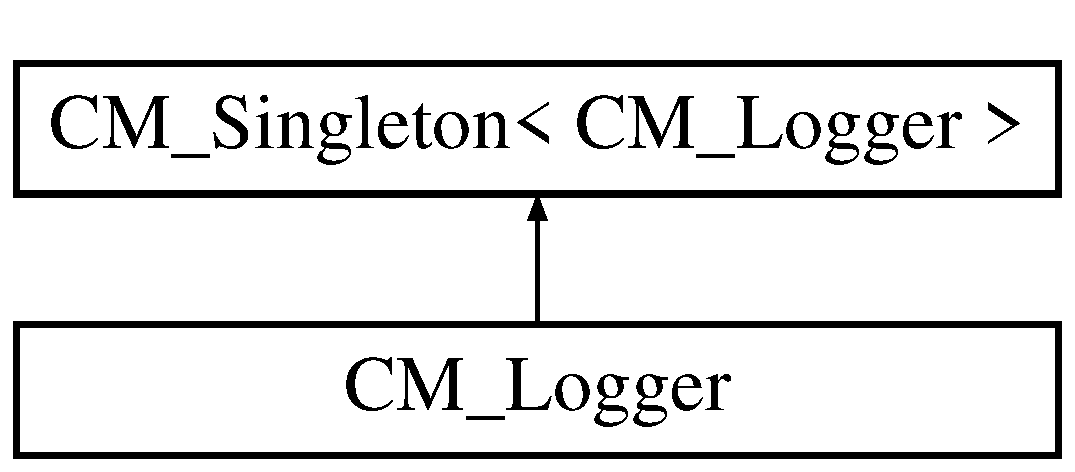
\includegraphics[height=2.000000cm]{class_c_m___logger}
\end{center}
\end{figure}
\subsection*{Classes}
\begin{DoxyCompactItemize}
\item 
class \hyperlink{class_c_m___logger_1_1_message}{Message}
\begin{DoxyCompactList}\small\item\em Encapsulates a message used by \hyperlink{class_c_m___logger}{C\+M\+\_\+\+Logger}. \end{DoxyCompactList}\end{DoxyCompactItemize}
\subsection*{Public Types}
\begin{DoxyCompactItemize}
\item 
enum \hyperlink{class_c_m___logger_ac2e71ba1ec4f24a09693eeae7b77611c}{Status} \{ {\bfseries Log}, 
{\bfseries Warning}, 
{\bfseries Error}
 \}\begin{DoxyCompactList}\small\item\em The status level of the message. \end{DoxyCompactList}
\end{DoxyCompactItemize}
\subsection*{Public Member Functions}
\begin{DoxyCompactItemize}
\item 
void \hyperlink{class_c_m___logger_a0fc384c005b14bcb9364fee0b82cfd96}{Log} (object message)
\begin{DoxyCompactList}\small\item\em Log the specified message with default log status. \end{DoxyCompactList}\item 
void \hyperlink{class_c_m___logger_a9000aa99a894afb7002eff79cf788483}{Log} (object context, object message)
\begin{DoxyCompactList}\small\item\em Log the message with the specified context. \end{DoxyCompactList}\item 
void \hyperlink{class_c_m___logger_ad08aaafdb501fce63a5fac80e2077e44}{Log} (object message, \hyperlink{class_c_m___logger_ac2e71ba1ec4f24a09693eeae7b77611c}{Status} status)
\begin{DoxyCompactList}\small\item\em Uses a lookup to either write a log, warning, or error based on the status. \end{DoxyCompactList}\end{DoxyCompactItemize}
\subsection*{Additional Inherited Members}


\subsection{Detailed Description}
Simple logging class used by the Coroutine Manager. 



\subsection{Member Enumeration Documentation}
\hypertarget{class_c_m___logger_ac2e71ba1ec4f24a09693eeae7b77611c}{}\index{C\+M\+\_\+\+Logger@{C\+M\+\_\+\+Logger}!Status@{Status}}
\index{Status@{Status}!C\+M\+\_\+\+Logger@{C\+M\+\_\+\+Logger}}
\subsubsection[{Status}]{\setlength{\rightskip}{0pt plus 5cm}enum {\bf C\+M\+\_\+\+Logger.\+Status}\hspace{0.3cm}{\ttfamily [strong]}}\label{class_c_m___logger_ac2e71ba1ec4f24a09693eeae7b77611c}


The status level of the message. 



\subsection{Member Function Documentation}
\hypertarget{class_c_m___logger_a0fc384c005b14bcb9364fee0b82cfd96}{}\index{C\+M\+\_\+\+Logger@{C\+M\+\_\+\+Logger}!Log@{Log}}
\index{Log@{Log}!C\+M\+\_\+\+Logger@{C\+M\+\_\+\+Logger}}
\subsubsection[{Log(object message)}]{\setlength{\rightskip}{0pt plus 5cm}void C\+M\+\_\+\+Logger.\+Log (
\begin{DoxyParamCaption}
\item[{object}]{message}
\end{DoxyParamCaption}
)}\label{class_c_m___logger_a0fc384c005b14bcb9364fee0b82cfd96}


Log the specified message with default log status. 


\begin{DoxyParams}{Parameters}
{\em message} & \hyperlink{class_c_m___logger_1_1_message}{Message}.\\
\hline
\end{DoxyParams}
\hypertarget{class_c_m___logger_a9000aa99a894afb7002eff79cf788483}{}\index{C\+M\+\_\+\+Logger@{C\+M\+\_\+\+Logger}!Log@{Log}}
\index{Log@{Log}!C\+M\+\_\+\+Logger@{C\+M\+\_\+\+Logger}}
\subsubsection[{Log(object context, object message)}]{\setlength{\rightskip}{0pt plus 5cm}void C\+M\+\_\+\+Logger.\+Log (
\begin{DoxyParamCaption}
\item[{object}]{context, }
\item[{object}]{message}
\end{DoxyParamCaption}
)}\label{class_c_m___logger_a9000aa99a894afb7002eff79cf788483}


Log the message with the specified context. 


\begin{DoxyParams}{Parameters}
{\em context} & Context i.\+e. the calling class.\\
\hline
{\em message} & \hyperlink{class_c_m___logger_1_1_message}{Message}.\\
\hline
\end{DoxyParams}
\hypertarget{class_c_m___logger_ad08aaafdb501fce63a5fac80e2077e44}{}\index{C\+M\+\_\+\+Logger@{C\+M\+\_\+\+Logger}!Log@{Log}}
\index{Log@{Log}!C\+M\+\_\+\+Logger@{C\+M\+\_\+\+Logger}}
\subsubsection[{Log(object message, Status status)}]{\setlength{\rightskip}{0pt plus 5cm}void C\+M\+\_\+\+Logger.\+Log (
\begin{DoxyParamCaption}
\item[{object}]{message, }
\item[{{\bf Status}}]{status}
\end{DoxyParamCaption}
)}\label{class_c_m___logger_ad08aaafdb501fce63a5fac80e2077e44}


Uses a lookup to either write a log, warning, or error based on the status. 


\begin{DoxyParams}{Parameters}
{\em message} & \hyperlink{class_c_m___logger_1_1_message}{Message}.\\
\hline
{\em status} & Status.\\
\hline
\end{DoxyParams}


The documentation for this class was generated from the following file\+:\begin{DoxyCompactItemize}
\item 
C\+M\+\_\+\+Logger.\+cs\end{DoxyCompactItemize}

\hypertarget{class_c_m___queue_event_args}{}\section{C\+M\+\_\+\+Queue\+Event\+Args Class Reference}
\label{class_c_m___queue_event_args}\index{C\+M\+\_\+\+Queue\+Event\+Args@{C\+M\+\_\+\+Queue\+Event\+Args}}


Arguements used by events raised by \hyperlink{class_c_m___job_queue}{C\+M\+\_\+\+Job\+Queue}.  


Inheritance diagram for C\+M\+\_\+\+Queue\+Event\+Args\+:\begin{figure}[H]
\begin{center}
\leavevmode
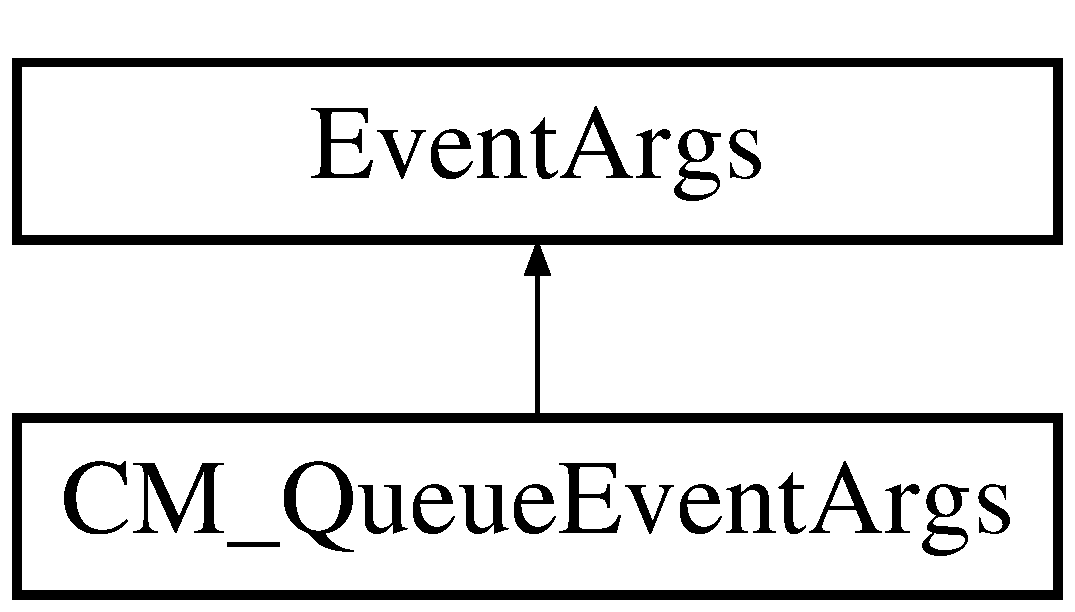
\includegraphics[height=2.000000cm]{class_c_m___queue_event_args}
\end{center}
\end{figure}
\subsection*{Public Member Functions}
\begin{DoxyCompactItemize}
\item 
\hyperlink{class_c_m___queue_event_args_a4345d4c604133866fab4bfd40143f70b}{C\+M\+\_\+\+Queue\+Event\+Args} (\hyperlink{class_c_m___job}{C\+M\+\_\+\+Job}\mbox{[}$\,$\mbox{]} \hyperlink{class_c_m___queue_event_args_a9a7016a83b4d77bfede3932565c13704}{queued\+Jobs}, \hyperlink{class_c_m___job}{C\+M\+\_\+\+Job}\mbox{[}$\,$\mbox{]} \hyperlink{class_c_m___queue_event_args_a89e1c990b52231168f5534204edfa25a}{completed\+Jobs}, \hyperlink{class_c_m___job_queue}{C\+M\+\_\+\+Job\+Queue} job\+Queue)
\begin{DoxyCompactList}\small\item\em Initializes a new instance of the \hyperlink{class_c_m___queue_event_args}{C\+M\+\_\+\+Queue\+Event\+Args} class. \end{DoxyCompactList}\end{DoxyCompactItemize}
\subsection*{Properties}
\begin{DoxyCompactItemize}
\item 
bool \hyperlink{class_c_m___queue_event_args_abc07a71f168a798661e040ad0f824591}{has\+Jobs\+In\+Queue}\hspace{0.3cm}{\ttfamily  \mbox{[}get\mbox{]}}
\begin{DoxyCompactList}\small\item\em Gets a value indicating whether this \hyperlink{class_c_m___queue_event_args}{C\+M\+\_\+\+Queue\+Event\+Args} has jobs in queue. \end{DoxyCompactList}\item 
\hyperlink{class_c_m___job}{C\+M\+\_\+\+Job}\mbox{[}$\,$\mbox{]} \hyperlink{class_c_m___queue_event_args_a9a7016a83b4d77bfede3932565c13704}{queued\+Jobs}\hspace{0.3cm}{\ttfamily  \mbox{[}get\mbox{]}}
\begin{DoxyCompactList}\small\item\em Gets the queued jobs. \end{DoxyCompactList}\item 
bool \hyperlink{class_c_m___queue_event_args_afa1760a1c067cea569209cf7458d1e5b}{has\+Completed\+Jobs}\hspace{0.3cm}{\ttfamily  \mbox{[}get\mbox{]}}
\begin{DoxyCompactList}\small\item\em Gets a value indicating whether this \hyperlink{class_c_m___queue_event_args}{C\+M\+\_\+\+Queue\+Event\+Args} has completed jobs. \end{DoxyCompactList}\item 
\hyperlink{class_c_m___job}{C\+M\+\_\+\+Job}\mbox{[}$\,$\mbox{]} \hyperlink{class_c_m___queue_event_args_a89e1c990b52231168f5534204edfa25a}{completed\+Jobs}\hspace{0.3cm}{\ttfamily  \mbox{[}get\mbox{]}}
\begin{DoxyCompactList}\small\item\em Gets the completed jobs. \end{DoxyCompactList}\item 
\hypertarget{class_c_m___queue_event_args_a4712e29b49def5bf891e70cb05182dbe}{}\hyperlink{class_c_m___job_queue}{C\+M\+\_\+\+Job\+Queue} {\bfseries job\+Queue}\hspace{0.3cm}{\ttfamily  \mbox{[}get\mbox{]}}\label{class_c_m___queue_event_args_a4712e29b49def5bf891e70cb05182dbe}

\end{DoxyCompactItemize}


\subsection{Detailed Description}
Arguements used by events raised by \hyperlink{class_c_m___job_queue}{C\+M\+\_\+\+Job\+Queue}. 



\subsection{Constructor \& Destructor Documentation}
\hypertarget{class_c_m___queue_event_args_a4345d4c604133866fab4bfd40143f70b}{}\index{C\+M\+\_\+\+Queue\+Event\+Args@{C\+M\+\_\+\+Queue\+Event\+Args}!C\+M\+\_\+\+Queue\+Event\+Args@{C\+M\+\_\+\+Queue\+Event\+Args}}
\index{C\+M\+\_\+\+Queue\+Event\+Args@{C\+M\+\_\+\+Queue\+Event\+Args}!C\+M\+\_\+\+Queue\+Event\+Args@{C\+M\+\_\+\+Queue\+Event\+Args}}
\subsubsection[{C\+M\+\_\+\+Queue\+Event\+Args(\+C\+M\+\_\+\+Job[] queued\+Jobs, C\+M\+\_\+\+Job[] completed\+Jobs, C\+M\+\_\+\+Job\+Queue job\+Queue)}]{\setlength{\rightskip}{0pt plus 5cm}C\+M\+\_\+\+Queue\+Event\+Args.\+C\+M\+\_\+\+Queue\+Event\+Args (
\begin{DoxyParamCaption}
\item[{{\bf C\+M\+\_\+\+Job}\mbox{[}$\,$\mbox{]}}]{queued\+Jobs, }
\item[{{\bf C\+M\+\_\+\+Job}\mbox{[}$\,$\mbox{]}}]{completed\+Jobs, }
\item[{{\bf C\+M\+\_\+\+Job\+Queue}}]{job\+Queue}
\end{DoxyParamCaption}
)}\label{class_c_m___queue_event_args_a4345d4c604133866fab4bfd40143f70b}


Initializes a new instance of the \hyperlink{class_c_m___queue_event_args}{C\+M\+\_\+\+Queue\+Event\+Args} class. 


\begin{DoxyParams}{Parameters}
{\em queued\+Jobs} & Queued jobs.\\
\hline
{\em completed\+Jobs} & Completed jobs.\\
\hline
\end{DoxyParams}


\subsection{Property Documentation}
\hypertarget{class_c_m___queue_event_args_a89e1c990b52231168f5534204edfa25a}{}\index{C\+M\+\_\+\+Queue\+Event\+Args@{C\+M\+\_\+\+Queue\+Event\+Args}!completed\+Jobs@{completed\+Jobs}}
\index{completed\+Jobs@{completed\+Jobs}!C\+M\+\_\+\+Queue\+Event\+Args@{C\+M\+\_\+\+Queue\+Event\+Args}}
\subsubsection[{completed\+Jobs}]{\setlength{\rightskip}{0pt plus 5cm}{\bf C\+M\+\_\+\+Job} \mbox{[}$\,$\mbox{]} C\+M\+\_\+\+Queue\+Event\+Args.\+completed\+Jobs\hspace{0.3cm}{\ttfamily [get]}}\label{class_c_m___queue_event_args_a89e1c990b52231168f5534204edfa25a}


Gets the completed jobs. 

The completed jobs.\hypertarget{class_c_m___queue_event_args_afa1760a1c067cea569209cf7458d1e5b}{}\index{C\+M\+\_\+\+Queue\+Event\+Args@{C\+M\+\_\+\+Queue\+Event\+Args}!has\+Completed\+Jobs@{has\+Completed\+Jobs}}
\index{has\+Completed\+Jobs@{has\+Completed\+Jobs}!C\+M\+\_\+\+Queue\+Event\+Args@{C\+M\+\_\+\+Queue\+Event\+Args}}
\subsubsection[{has\+Completed\+Jobs}]{\setlength{\rightskip}{0pt plus 5cm}bool C\+M\+\_\+\+Queue\+Event\+Args.\+has\+Completed\+Jobs\hspace{0.3cm}{\ttfamily [get]}}\label{class_c_m___queue_event_args_afa1760a1c067cea569209cf7458d1e5b}


Gets a value indicating whether this \hyperlink{class_c_m___queue_event_args}{C\+M\+\_\+\+Queue\+Event\+Args} has completed jobs. 

{\ttfamily true} if has completed jobs; otherwise, {\ttfamily false}.\hypertarget{class_c_m___queue_event_args_abc07a71f168a798661e040ad0f824591}{}\index{C\+M\+\_\+\+Queue\+Event\+Args@{C\+M\+\_\+\+Queue\+Event\+Args}!has\+Jobs\+In\+Queue@{has\+Jobs\+In\+Queue}}
\index{has\+Jobs\+In\+Queue@{has\+Jobs\+In\+Queue}!C\+M\+\_\+\+Queue\+Event\+Args@{C\+M\+\_\+\+Queue\+Event\+Args}}
\subsubsection[{has\+Jobs\+In\+Queue}]{\setlength{\rightskip}{0pt plus 5cm}bool C\+M\+\_\+\+Queue\+Event\+Args.\+has\+Jobs\+In\+Queue\hspace{0.3cm}{\ttfamily [get]}}\label{class_c_m___queue_event_args_abc07a71f168a798661e040ad0f824591}


Gets a value indicating whether this \hyperlink{class_c_m___queue_event_args}{C\+M\+\_\+\+Queue\+Event\+Args} has jobs in queue. 

{\ttfamily true} if has jobs in queue; otherwise, {\ttfamily false}.\hypertarget{class_c_m___queue_event_args_a9a7016a83b4d77bfede3932565c13704}{}\index{C\+M\+\_\+\+Queue\+Event\+Args@{C\+M\+\_\+\+Queue\+Event\+Args}!queued\+Jobs@{queued\+Jobs}}
\index{queued\+Jobs@{queued\+Jobs}!C\+M\+\_\+\+Queue\+Event\+Args@{C\+M\+\_\+\+Queue\+Event\+Args}}
\subsubsection[{queued\+Jobs}]{\setlength{\rightskip}{0pt plus 5cm}{\bf C\+M\+\_\+\+Job} \mbox{[}$\,$\mbox{]} C\+M\+\_\+\+Queue\+Event\+Args.\+queued\+Jobs\hspace{0.3cm}{\ttfamily [get]}}\label{class_c_m___queue_event_args_a9a7016a83b4d77bfede3932565c13704}


Gets the queued jobs. 

The queued jobs.

The documentation for this class was generated from the following file\+:\begin{DoxyCompactItemize}
\item 
C\+M\+\_\+\+Queue\+Event\+Args.\+cs\end{DoxyCompactItemize}

\hypertarget{class_c_m___singleton}{}\section{C\+M\+\_\+\+Singleton$<$ T $>$ Class Template Reference}
\label{class_c_m___singleton}\index{C\+M\+\_\+\+Singleton$<$ T $>$@{C\+M\+\_\+\+Singleton$<$ T $>$}}


A base class for any Singleton. Provides global singular access to a Mono\+Behaviour.  


Inheritance diagram for C\+M\+\_\+\+Singleton$<$ T $>$\+:\begin{figure}[H]
\begin{center}
\leavevmode
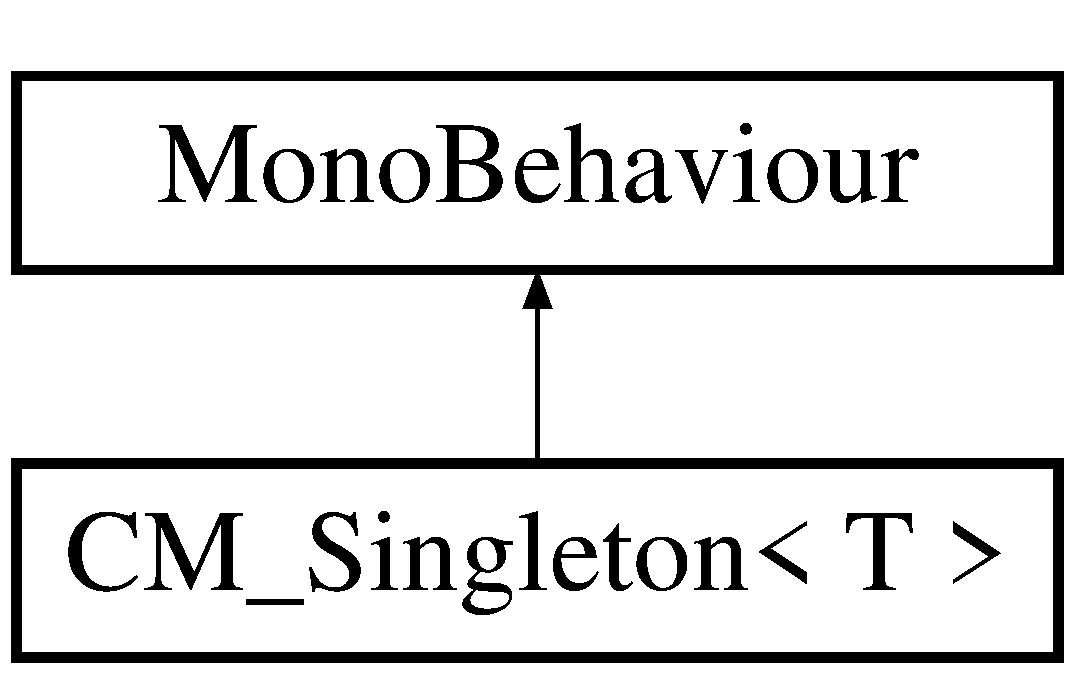
\includegraphics[height=2.000000cm]{class_c_m___singleton}
\end{center}
\end{figure}
\subsection*{Protected Member Functions}
\begin{DoxyCompactItemize}
\item 
\hypertarget{class_c_m___singleton_af232ba062023581cc42e779598abe148}{}virtual void {\bfseries On\+Destroy} ()\label{class_c_m___singleton_af232ba062023581cc42e779598abe148}

\item 
\hypertarget{class_c_m___singleton_a902c7afbd9bfce107ff99c137dbf8d5f}{}virtual void {\bfseries On\+Application\+Quit} ()\label{class_c_m___singleton_a902c7afbd9bfce107ff99c137dbf8d5f}

\end{DoxyCompactItemize}
\subsection*{Properties}
\begin{DoxyCompactItemize}
\item 
static bool \hyperlink{class_c_m___singleton_a2d488ea5c08e0b2a2bd78e3e8658f0d4}{Is\+Destroyed}\hspace{0.3cm}{\ttfamily  \mbox{[}get\mbox{]}}
\begin{DoxyCompactList}\small\item\em Gets a value indicating whether this instance is destroyed. \end{DoxyCompactList}\item 
static T \hyperlink{class_c_m___singleton_af2377c7977dd169962d9b76dc0fb2f45}{instance}\hspace{0.3cm}{\ttfamily  \mbox{[}get\mbox{]}}
\begin{DoxyCompactList}\small\item\em Gets the instance. The instance is created if not currently past of the scene. \end{DoxyCompactList}\end{DoxyCompactItemize}


\subsection{Detailed Description}
A base class for any Singleton. Provides global singular access to a Mono\+Behaviour. 

\begin{Desc}
\item[Type Constraints]\begin{description}
\item[{\em T} : {\em Mono\+Behaviour}]\end{description}
\end{Desc}


\subsection{Property Documentation}
\hypertarget{class_c_m___singleton_af2377c7977dd169962d9b76dc0fb2f45}{}\index{C\+M\+\_\+\+Singleton@{C\+M\+\_\+\+Singleton}!instance@{instance}}
\index{instance@{instance}!C\+M\+\_\+\+Singleton@{C\+M\+\_\+\+Singleton}}
\subsubsection[{instance}]{\setlength{\rightskip}{0pt plus 5cm}T {\bf C\+M\+\_\+\+Singleton}$<$ T $>$.instance\hspace{0.3cm}{\ttfamily [static]}, {\ttfamily [get]}}\label{class_c_m___singleton_af2377c7977dd169962d9b76dc0fb2f45}


Gets the instance. The instance is created if not currently past of the scene. 

The instance.\hypertarget{class_c_m___singleton_a2d488ea5c08e0b2a2bd78e3e8658f0d4}{}\index{C\+M\+\_\+\+Singleton@{C\+M\+\_\+\+Singleton}!Is\+Destroyed@{Is\+Destroyed}}
\index{Is\+Destroyed@{Is\+Destroyed}!C\+M\+\_\+\+Singleton@{C\+M\+\_\+\+Singleton}}
\subsubsection[{Is\+Destroyed}]{\setlength{\rightskip}{0pt plus 5cm}bool {\bf C\+M\+\_\+\+Singleton}$<$ T $>$.Is\+Destroyed\hspace{0.3cm}{\ttfamily [static]}, {\ttfamily [get]}}\label{class_c_m___singleton_a2d488ea5c08e0b2a2bd78e3e8658f0d4}


Gets a value indicating whether this instance is destroyed. 

{\ttfamily true} if is destroyed; otherwise, {\ttfamily false}.

The documentation for this class was generated from the following file\+:\begin{DoxyCompactItemize}
\item 
C\+M\+\_\+\+Singleton.\+cs\end{DoxyCompactItemize}

\hypertarget{class_example_character_damage}{}\section{Example\+Character\+Damage Class Reference}
\label{class_example_character_damage}\index{Example\+Character\+Damage@{Example\+Character\+Damage}}


Example character with action queue.  


Inheritance diagram for Example\+Character\+Damage\+:\begin{figure}[H]
\begin{center}
\leavevmode
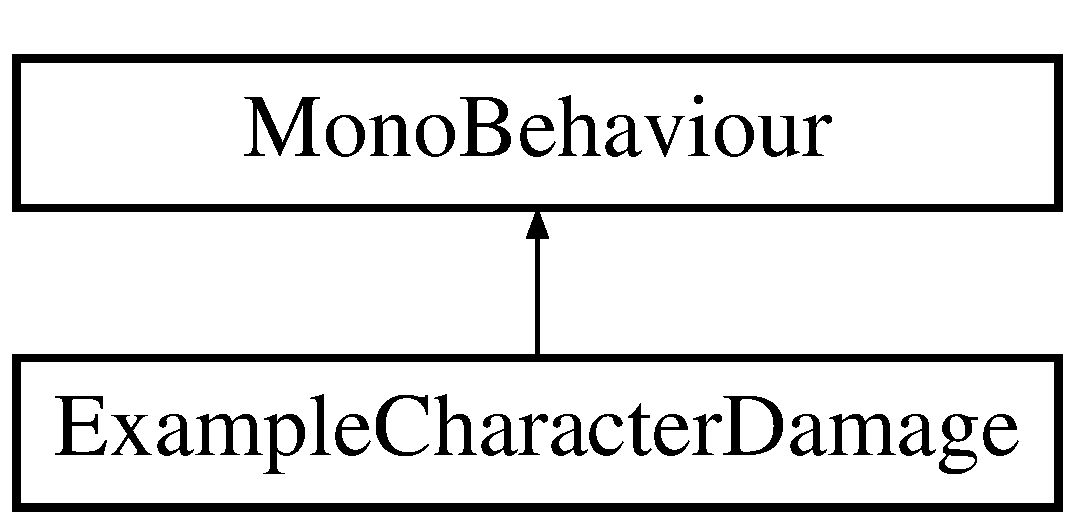
\includegraphics[height=2.000000cm]{class_example_character_damage}
\end{center}
\end{figure}
\subsection*{Public Member Functions}
\begin{DoxyCompactItemize}
\item 
void \hyperlink{class_example_character_damage_a0befb25f1d266a74f6ea9b2bb25b8d6d}{Add\+Action\+To\+Queue} (\hyperlink{class_c_m___job}{C\+M\+\_\+\+Job} action)
\begin{DoxyCompactList}\small\item\em Adds the action to the current queue. An action can be any coroutine you want. \end{DoxyCompactList}\item 
I\+Enumerator \hyperlink{class_example_character_damage_af25a43f4182d205ca89e73d7dc0794f3}{Apply\+Damage} (string damage\+Type, float time)
\begin{DoxyCompactList}\small\item\em Simulates the application of damage over time. \end{DoxyCompactList}\item 
I\+Enumerator \hyperlink{class_example_character_damage_aeb1574e48eac8ed8c211b5ea0d488782}{Restore\+Health} (float time)
\begin{DoxyCompactList}\small\item\em Simulates restoring of health over time. \end{DoxyCompactList}\end{DoxyCompactItemize}
\subsection*{Public Attributes}
\begin{DoxyCompactItemize}
\item 
\hypertarget{class_example_character_damage_a9f184018de86afde217ec6978018874d}{}float {\bfseries health} = 20f\label{class_example_character_damage_a9f184018de86afde217ec6978018874d}

\end{DoxyCompactItemize}


\subsection{Detailed Description}
Example character with action queue. 



\subsection{Member Function Documentation}
\hypertarget{class_example_character_damage_a0befb25f1d266a74f6ea9b2bb25b8d6d}{}\index{Example\+Character\+Damage@{Example\+Character\+Damage}!Add\+Action\+To\+Queue@{Add\+Action\+To\+Queue}}
\index{Add\+Action\+To\+Queue@{Add\+Action\+To\+Queue}!Example\+Character\+Damage@{Example\+Character\+Damage}}
\subsubsection[{Add\+Action\+To\+Queue(\+C\+M\+\_\+\+Job action)}]{\setlength{\rightskip}{0pt plus 5cm}void Example\+Character\+Damage.\+Add\+Action\+To\+Queue (
\begin{DoxyParamCaption}
\item[{{\bf C\+M\+\_\+\+Job}}]{action}
\end{DoxyParamCaption}
)}\label{class_example_character_damage_a0befb25f1d266a74f6ea9b2bb25b8d6d}


Adds the action to the current queue. An action can be any coroutine you want. 


\begin{DoxyParams}{Parameters}
{\em action} & Action.\\
\hline
\end{DoxyParams}
\hypertarget{class_example_character_damage_af25a43f4182d205ca89e73d7dc0794f3}{}\index{Example\+Character\+Damage@{Example\+Character\+Damage}!Apply\+Damage@{Apply\+Damage}}
\index{Apply\+Damage@{Apply\+Damage}!Example\+Character\+Damage@{Example\+Character\+Damage}}
\subsubsection[{Apply\+Damage(string damage\+Type, float time)}]{\setlength{\rightskip}{0pt plus 5cm}I\+Enumerator Example\+Character\+Damage.\+Apply\+Damage (
\begin{DoxyParamCaption}
\item[{string}]{damage\+Type, }
\item[{float}]{time}
\end{DoxyParamCaption}
)}\label{class_example_character_damage_af25a43f4182d205ca89e73d7dc0794f3}


Simulates the application of damage over time. 

\begin{DoxyReturn}{Returns}
The damage.
\end{DoxyReturn}

\begin{DoxyParams}{Parameters}
{\em damage\+Type} & Damage type.\\
\hline
{\em time} & Time.\\
\hline
\end{DoxyParams}
\hypertarget{class_example_character_damage_aeb1574e48eac8ed8c211b5ea0d488782}{}\index{Example\+Character\+Damage@{Example\+Character\+Damage}!Restore\+Health@{Restore\+Health}}
\index{Restore\+Health@{Restore\+Health}!Example\+Character\+Damage@{Example\+Character\+Damage}}
\subsubsection[{Restore\+Health(float time)}]{\setlength{\rightskip}{0pt plus 5cm}I\+Enumerator Example\+Character\+Damage.\+Restore\+Health (
\begin{DoxyParamCaption}
\item[{float}]{time}
\end{DoxyParamCaption}
)}\label{class_example_character_damage_aeb1574e48eac8ed8c211b5ea0d488782}


Simulates restoring of health over time. 

\begin{DoxyReturn}{Returns}
The health.
\end{DoxyReturn}

\begin{DoxyParams}{Parameters}
{\em time} & Time.\\
\hline
\end{DoxyParams}


The documentation for this class was generated from the following file\+:\begin{DoxyCompactItemize}
\item 
Example\+Character\+Damage.\+cs\end{DoxyCompactItemize}

\hypertarget{class_example_character_movement}{}\section{Example\+Character\+Movement Class Reference}
\label{class_example_character_movement}\index{Example\+Character\+Movement@{Example\+Character\+Movement}}


Example Script. A simple script showing how you can use \hyperlink{class_c_m___job_queue}{C\+M\+\_\+\+Job\+Queue} to create easily repeatable character movement.  


Inheritance diagram for Example\+Character\+Movement\+:\begin{figure}[H]
\begin{center}
\leavevmode
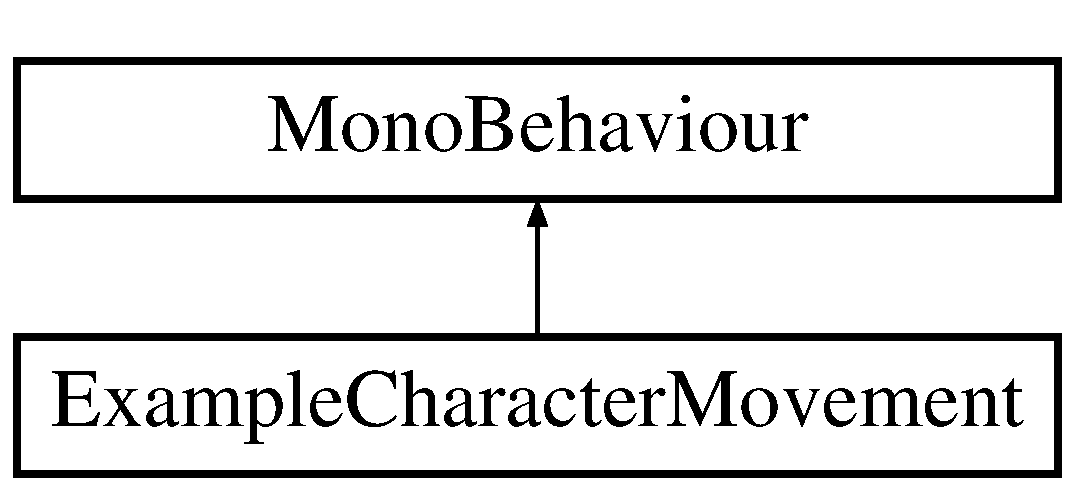
\includegraphics[height=2.000000cm]{class_example_character_movement}
\end{center}
\end{figure}
\subsection*{Public Attributes}
\begin{DoxyCompactItemize}
\item 
float \hyperlink{class_example_character_movement_a2b35a1171dcecd39d3a8f60c5d5b037a}{move\+Speed} = 10f
\begin{DoxyCompactList}\small\item\em The movement speed of the character. \end{DoxyCompactList}\end{DoxyCompactItemize}


\subsection{Detailed Description}
Example Script. A simple script showing how you can use \hyperlink{class_c_m___job_queue}{C\+M\+\_\+\+Job\+Queue} to create easily repeatable character movement. 



\subsection{Member Data Documentation}
\hypertarget{class_example_character_movement_a2b35a1171dcecd39d3a8f60c5d5b037a}{}\index{Example\+Character\+Movement@{Example\+Character\+Movement}!move\+Speed@{move\+Speed}}
\index{move\+Speed@{move\+Speed}!Example\+Character\+Movement@{Example\+Character\+Movement}}
\subsubsection[{move\+Speed}]{\setlength{\rightskip}{0pt plus 5cm}float Example\+Character\+Movement.\+move\+Speed = 10f}\label{class_example_character_movement_a2b35a1171dcecd39d3a8f60c5d5b037a}


The movement speed of the character. 



The documentation for this class was generated from the following file\+:\begin{DoxyCompactItemize}
\item 
Example\+Character\+Movement.\+cs\end{DoxyCompactItemize}

\hypertarget{class_example_continous_spawner}{}\section{Example\+Continous\+Spawner Class Reference}
\label{class_example_continous_spawner}\index{Example\+Continous\+Spawner@{Example\+Continous\+Spawner}}


Example Script. Used to spawn a number of objects using \hyperlink{class_c_m___job}{C\+M\+\_\+\+Job}.  


Inheritance diagram for Example\+Continous\+Spawner\+:\begin{figure}[H]
\begin{center}
\leavevmode
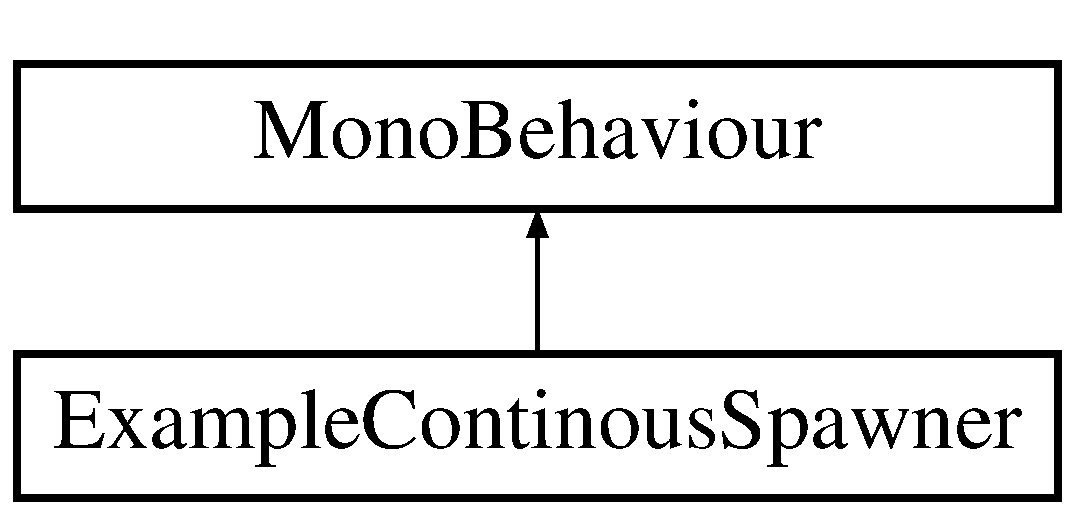
\includegraphics[height=2.000000cm]{class_example_continous_spawner}
\end{center}
\end{figure}
\subsection*{Public Attributes}
\begin{DoxyCompactItemize}
\item 
Game\+Object \hyperlink{class_example_continous_spawner_ad4617f03c5d944453742b8ce30b25396}{prefab}
\begin{DoxyCompactList}\small\item\em The prefab to spawn. \end{DoxyCompactList}\item 
int \hyperlink{class_example_continous_spawner_af4226a3d4c13b1e447003b3a45e5638f}{num\+To\+Spawn} = 200
\begin{DoxyCompactList}\small\item\em The number of objects to spawn. \end{DoxyCompactList}\item 
float \hyperlink{class_example_continous_spawner_a99d962ed337668df7b9ce0a99042eec1}{time\+Between\+Spawns} = 0.\+1f
\begin{DoxyCompactList}\small\item\em The time between spawns. \end{DoxyCompactList}\end{DoxyCompactItemize}


\subsection{Detailed Description}
Example Script. Used to spawn a number of objects using \hyperlink{class_c_m___job}{C\+M\+\_\+\+Job}. 



\subsection{Member Data Documentation}
\hypertarget{class_example_continous_spawner_af4226a3d4c13b1e447003b3a45e5638f}{}\index{Example\+Continous\+Spawner@{Example\+Continous\+Spawner}!num\+To\+Spawn@{num\+To\+Spawn}}
\index{num\+To\+Spawn@{num\+To\+Spawn}!Example\+Continous\+Spawner@{Example\+Continous\+Spawner}}
\subsubsection[{num\+To\+Spawn}]{\setlength{\rightskip}{0pt plus 5cm}int Example\+Continous\+Spawner.\+num\+To\+Spawn = 200}\label{class_example_continous_spawner_af4226a3d4c13b1e447003b3a45e5638f}


The number of objects to spawn. 

\hypertarget{class_example_continous_spawner_ad4617f03c5d944453742b8ce30b25396}{}\index{Example\+Continous\+Spawner@{Example\+Continous\+Spawner}!prefab@{prefab}}
\index{prefab@{prefab}!Example\+Continous\+Spawner@{Example\+Continous\+Spawner}}
\subsubsection[{prefab}]{\setlength{\rightskip}{0pt plus 5cm}Game\+Object Example\+Continous\+Spawner.\+prefab}\label{class_example_continous_spawner_ad4617f03c5d944453742b8ce30b25396}


The prefab to spawn. 

\hypertarget{class_example_continous_spawner_a99d962ed337668df7b9ce0a99042eec1}{}\index{Example\+Continous\+Spawner@{Example\+Continous\+Spawner}!time\+Between\+Spawns@{time\+Between\+Spawns}}
\index{time\+Between\+Spawns@{time\+Between\+Spawns}!Example\+Continous\+Spawner@{Example\+Continous\+Spawner}}
\subsubsection[{time\+Between\+Spawns}]{\setlength{\rightskip}{0pt plus 5cm}float Example\+Continous\+Spawner.\+time\+Between\+Spawns = 0.\+1f}\label{class_example_continous_spawner_a99d962ed337668df7b9ce0a99042eec1}


The time between spawns. 



The documentation for this class was generated from the following file\+:\begin{DoxyCompactItemize}
\item 
Example\+Continous\+Spawner.\+cs\end{DoxyCompactItemize}

\hypertarget{class_example_damage_applier}{}\section{Example\+Damage\+Applier Class Reference}
\label{class_example_damage_applier}\index{Example\+Damage\+Applier@{Example\+Damage\+Applier}}


Applies damage actions to the example character.  


Inheritance diagram for Example\+Damage\+Applier\+:\begin{figure}[H]
\begin{center}
\leavevmode
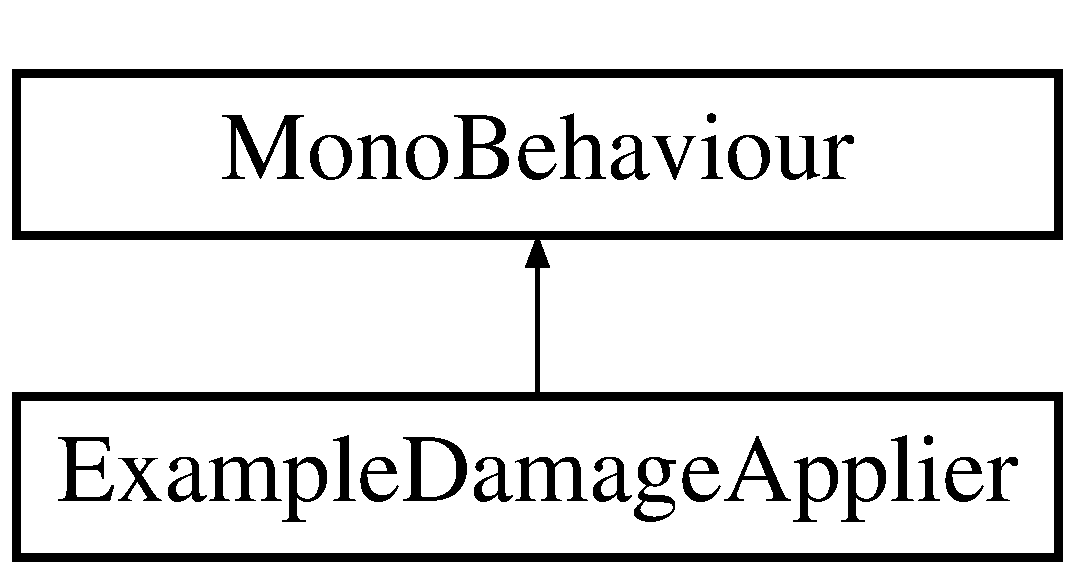
\includegraphics[height=2.000000cm]{class_example_damage_applier}
\end{center}
\end{figure}
\subsection*{Public Attributes}
\begin{DoxyCompactItemize}
\item 
\hyperlink{class_example_character_damage}{Example\+Character\+Damage} \hyperlink{class_example_damage_applier_a1275e973ce691cf54b0f3e5c1fa90007}{character}
\begin{DoxyCompactList}\small\item\em The character to apply damage actions to. \end{DoxyCompactList}\end{DoxyCompactItemize}


\subsection{Detailed Description}
Applies damage actions to the example character. 



\subsection{Member Data Documentation}
\hypertarget{class_example_damage_applier_a1275e973ce691cf54b0f3e5c1fa90007}{}\index{Example\+Damage\+Applier@{Example\+Damage\+Applier}!character@{character}}
\index{character@{character}!Example\+Damage\+Applier@{Example\+Damage\+Applier}}
\subsubsection[{character}]{\setlength{\rightskip}{0pt plus 5cm}{\bf Example\+Character\+Damage} Example\+Damage\+Applier.\+character}\label{class_example_damage_applier_a1275e973ce691cf54b0f3e5c1fa90007}


The character to apply damage actions to. 



The documentation for this class was generated from the following file\+:\begin{DoxyCompactItemize}
\item 
Example\+Damage\+Applier.\+cs\end{DoxyCompactItemize}

\hypertarget{class_example_g_u_i}{}\section{Example\+G\+U\+I Class Reference}
\label{class_example_g_u_i}\index{Example\+G\+U\+I@{Example\+G\+U\+I}}


Simple G\+U\+I controller. Uses a \hyperlink{class_c_m___job_queue}{C\+M\+\_\+\+Job\+Queue} to enqueue a number of gui actions.  


Inheritance diagram for Example\+G\+U\+I\+:\begin{figure}[H]
\begin{center}
\leavevmode
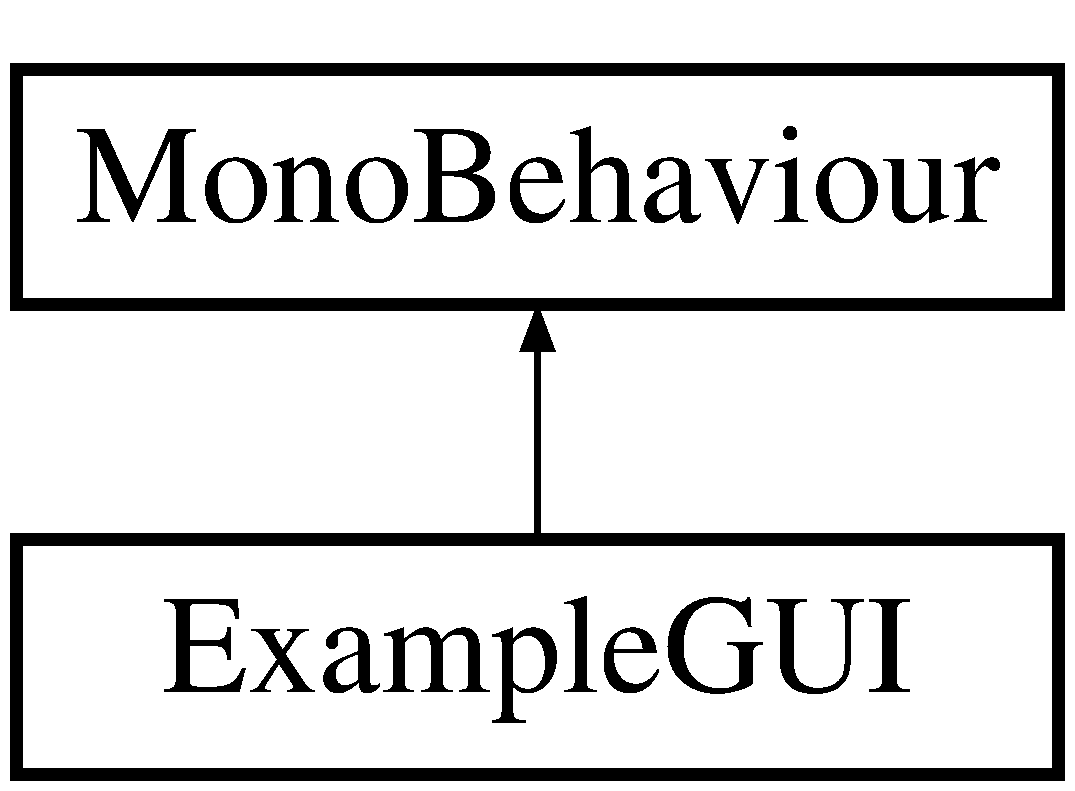
\includegraphics[height=2.000000cm]{class_example_g_u_i}
\end{center}
\end{figure}
\subsection*{Public Attributes}
\begin{DoxyCompactItemize}
\item 
Text \hyperlink{class_example_g_u_i_a2eaf69cbe810531fcc820e264c288698}{title\+Text}
\begin{DoxyCompactList}\small\item\em T\+He G\+U\+I text \end{DoxyCompactList}\end{DoxyCompactItemize}


\subsection{Detailed Description}
Simple G\+U\+I controller. Uses a \hyperlink{class_c_m___job_queue}{C\+M\+\_\+\+Job\+Queue} to enqueue a number of gui actions. 



\subsection{Member Data Documentation}
\hypertarget{class_example_g_u_i_a2eaf69cbe810531fcc820e264c288698}{}\index{Example\+G\+U\+I@{Example\+G\+U\+I}!title\+Text@{title\+Text}}
\index{title\+Text@{title\+Text}!Example\+G\+U\+I@{Example\+G\+U\+I}}
\subsubsection[{title\+Text}]{\setlength{\rightskip}{0pt plus 5cm}Text Example\+G\+U\+I.\+title\+Text}\label{class_example_g_u_i_a2eaf69cbe810531fcc820e264c288698}


T\+He G\+U\+I text 



The documentation for this class was generated from the following file\+:\begin{DoxyCompactItemize}
\item 
Example\+G\+U\+I.\+cs\end{DoxyCompactItemize}

\hypertarget{class_example_job_manager_test}{}\section{Example\+Job\+Manager\+Test Class Reference}
\label{class_example_job_manager_test}\index{Example\+Job\+Manager\+Test@{Example\+Job\+Manager\+Test}}


Includes a number of methods to test the functionality of the \hyperlink{class_c_m___job_manager}{C\+M\+\_\+\+Job\+Manager} class. Each method showcases a particular functionality of the \hyperlink{class_c_m___job_manager}{C\+M\+\_\+\+Job\+Manager} that you can implement in your own projects.  


Inheritance diagram for Example\+Job\+Manager\+Test\+:\begin{figure}[H]
\begin{center}
\leavevmode
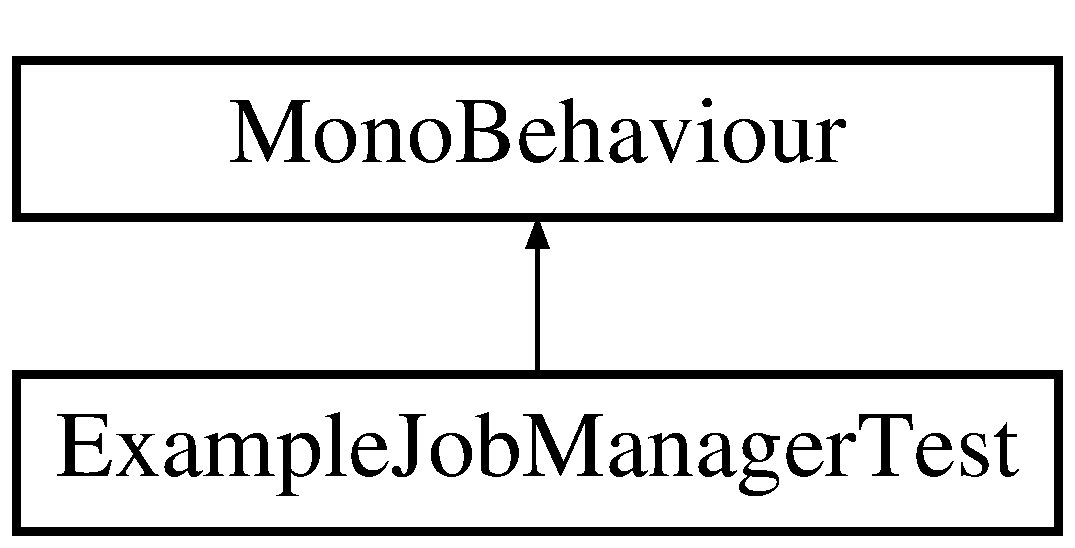
\includegraphics[height=2.000000cm]{class_example_job_manager_test}
\end{center}
\end{figure}
\subsection*{Public Member Functions}
\begin{DoxyCompactItemize}
\item 
void \hyperlink{class_example_job_manager_test_a2e12fad77a94ff2cbcc3b7da2cb16362}{Global\+Job\+Manager\+Event\+Test} ()
\begin{DoxyCompactList}\small\item\em Subscribes to each of the global managers events. Notify\+On\+Job\+Added\+: called everytime a job is added to the global manager, Notify\+On\+Job\+Removed\+: called everytime a job is removed, Notify\+On\+All\+Jobs\+Killed\+: called when \hyperlink{class_c_m___job_manager_ab5a27b84b4fd3893e1dc271570930e62}{C\+M\+\_\+\+Job\+Manager.\+Kill\+All} is invoked, Notify\+On\+All\+Jobs\+Resumed\+: called when \hyperlink{class_c_m___job_manager_a838152b138f04a0c4c254f3b56bd31fe}{C\+M\+\_\+\+Job\+Manager.\+Resume\+All} is called, Notify\+On\+All\+Jobs\+Paused\+: called when \hyperlink{class_c_m___job_manager_ab1e48755bb929871595acfca595ae01b}{C\+M\+\_\+\+Job\+Manager.\+Pause\+All} is invoked, and Notify\+On\+All\+Jobs\+Cleared\+: called when \hyperlink{class_c_m___job_manager_a7684d8a980b6dd3004feb35e978e2163}{C\+M\+\_\+\+Job\+Manager.\+Clear\+Job\+List} is invoked. \end{DoxyCompactList}\item 
void \hyperlink{class_example_job_manager_test_ae4b00ba638975a806c58d4fea116406b}{Global\+Job\+Start\+Test} ()
\begin{DoxyCompactList}\small\item\em Starts the test job. \end{DoxyCompactList}\item 
void \hyperlink{class_example_job_manager_test_ab38e4ec613dc3f50c4204ac3e1963dac}{Global\+Job\+Pause\+Test} ()
\begin{DoxyCompactList}\small\item\em Pauses the test job. \end{DoxyCompactList}\item 
void \hyperlink{class_example_job_manager_test_a2ba384ab22381d74acbf229ad81f5e6e}{Global\+Job\+Resume\+Test} ()
\begin{DoxyCompactList}\small\item\em Resumes the test job. \end{DoxyCompactList}\item 
void \hyperlink{class_example_job_manager_test_ae9165213486f9d72a0fd0bfc59ab0ab4}{Global\+Job\+Stop\+Test} ()
\begin{DoxyCompactList}\small\item\em Stops the test job. This also removes the reference from the Job\+Manager. \end{DoxyCompactList}\item 
void \hyperlink{class_example_job_manager_test_a031ebb468ce25cdda0d946eda3a8108c}{Global\+Start\+All\+Test} ()
\begin{DoxyCompactList}\small\item\em Starts all jobs owned by the global Job\+Manager. \end{DoxyCompactList}\item 
void \hyperlink{class_example_job_manager_test_a90dd8a5a25c6ad18e507fca1967aca21}{Delayed\+Pause\+All\+Test} ()
\begin{DoxyCompactList}\small\item\em Pauses all jobs owned by the global Job\+Manager after 1 second has passed. \end{DoxyCompactList}\item 
void \hyperlink{class_example_job_manager_test_aa47f66fa961dbf64f689a7e1306ffafc}{Delayed\+Resume\+All\+Test} ()
\begin{DoxyCompactList}\small\item\em Resumes all jobs owned by the global Job\+Manager after 1.\+5 seconds have passed. \end{DoxyCompactList}\item 
void \hyperlink{class_example_job_manager_test_a6fb632a5a0a84a997e093b3cd04b1a1b}{Delayed\+Kill\+All\+Test} ()
\begin{DoxyCompactList}\small\item\em Kills all jobs owned by the global Job\+Manager after 2 seconds have passed. This also removes all references to those jobs from the Job\+Manager. \end{DoxyCompactList}\item 
void \hyperlink{class_example_job_manager_test_ae02ae80e68427cd8604e527982ee8b54}{Local\+Job\+Manager\+Test} ()
\begin{DoxyCompactList}\small\item\em Local job manager test. Creates a new local Job\+Manager, subscribes to \hyperlink{class_c_m___job_manager_a0f3c4dff8b782e1b64abcbb7dc19cd8a}{C\+M\+\_\+\+Job\+Manager.\+job\+Added} and \hyperlink{class_c_m___job_manager_a3a24d267ce0e6a09a2cf8f13429f2b73}{C\+M\+\_\+\+Job\+Manager.\+job\+Removed} events, adds a test job to the local Job\+Manager, and finally starts, pauses, resumes, and stops this test job. This is used to show that anything you can do with the glocal Job\+Manager you can also do with a local Job\+Manager. This is useful if you want to create seperate Job\+Managers for seperate parts of your codebase. \end{DoxyCompactList}\end{DoxyCompactItemize}


\subsection{Detailed Description}
Includes a number of methods to test the functionality of the \hyperlink{class_c_m___job_manager}{C\+M\+\_\+\+Job\+Manager} class. Each method showcases a particular functionality of the \hyperlink{class_c_m___job_manager}{C\+M\+\_\+\+Job\+Manager} that you can implement in your own projects. 



\subsection{Member Function Documentation}
\hypertarget{class_example_job_manager_test_a6fb632a5a0a84a997e093b3cd04b1a1b}{}\index{Example\+Job\+Manager\+Test@{Example\+Job\+Manager\+Test}!Delayed\+Kill\+All\+Test@{Delayed\+Kill\+All\+Test}}
\index{Delayed\+Kill\+All\+Test@{Delayed\+Kill\+All\+Test}!Example\+Job\+Manager\+Test@{Example\+Job\+Manager\+Test}}
\subsubsection[{Delayed\+Kill\+All\+Test()}]{\setlength{\rightskip}{0pt plus 5cm}void Example\+Job\+Manager\+Test.\+Delayed\+Kill\+All\+Test (
\begin{DoxyParamCaption}
{}
\end{DoxyParamCaption}
)}\label{class_example_job_manager_test_a6fb632a5a0a84a997e093b3cd04b1a1b}


Kills all jobs owned by the global Job\+Manager after 2 seconds have passed. This also removes all references to those jobs from the Job\+Manager. 

\hypertarget{class_example_job_manager_test_a90dd8a5a25c6ad18e507fca1967aca21}{}\index{Example\+Job\+Manager\+Test@{Example\+Job\+Manager\+Test}!Delayed\+Pause\+All\+Test@{Delayed\+Pause\+All\+Test}}
\index{Delayed\+Pause\+All\+Test@{Delayed\+Pause\+All\+Test}!Example\+Job\+Manager\+Test@{Example\+Job\+Manager\+Test}}
\subsubsection[{Delayed\+Pause\+All\+Test()}]{\setlength{\rightskip}{0pt plus 5cm}void Example\+Job\+Manager\+Test.\+Delayed\+Pause\+All\+Test (
\begin{DoxyParamCaption}
{}
\end{DoxyParamCaption}
)}\label{class_example_job_manager_test_a90dd8a5a25c6ad18e507fca1967aca21}


Pauses all jobs owned by the global Job\+Manager after 1 second has passed. 

\hypertarget{class_example_job_manager_test_aa47f66fa961dbf64f689a7e1306ffafc}{}\index{Example\+Job\+Manager\+Test@{Example\+Job\+Manager\+Test}!Delayed\+Resume\+All\+Test@{Delayed\+Resume\+All\+Test}}
\index{Delayed\+Resume\+All\+Test@{Delayed\+Resume\+All\+Test}!Example\+Job\+Manager\+Test@{Example\+Job\+Manager\+Test}}
\subsubsection[{Delayed\+Resume\+All\+Test()}]{\setlength{\rightskip}{0pt plus 5cm}void Example\+Job\+Manager\+Test.\+Delayed\+Resume\+All\+Test (
\begin{DoxyParamCaption}
{}
\end{DoxyParamCaption}
)}\label{class_example_job_manager_test_aa47f66fa961dbf64f689a7e1306ffafc}


Resumes all jobs owned by the global Job\+Manager after 1.\+5 seconds have passed. 

\hypertarget{class_example_job_manager_test_a2e12fad77a94ff2cbcc3b7da2cb16362}{}\index{Example\+Job\+Manager\+Test@{Example\+Job\+Manager\+Test}!Global\+Job\+Manager\+Event\+Test@{Global\+Job\+Manager\+Event\+Test}}
\index{Global\+Job\+Manager\+Event\+Test@{Global\+Job\+Manager\+Event\+Test}!Example\+Job\+Manager\+Test@{Example\+Job\+Manager\+Test}}
\subsubsection[{Global\+Job\+Manager\+Event\+Test()}]{\setlength{\rightskip}{0pt plus 5cm}void Example\+Job\+Manager\+Test.\+Global\+Job\+Manager\+Event\+Test (
\begin{DoxyParamCaption}
{}
\end{DoxyParamCaption}
)}\label{class_example_job_manager_test_a2e12fad77a94ff2cbcc3b7da2cb16362}


Subscribes to each of the global managers events. Notify\+On\+Job\+Added\+: called everytime a job is added to the global manager, Notify\+On\+Job\+Removed\+: called everytime a job is removed, Notify\+On\+All\+Jobs\+Killed\+: called when \hyperlink{class_c_m___job_manager_ab5a27b84b4fd3893e1dc271570930e62}{C\+M\+\_\+\+Job\+Manager.\+Kill\+All} is invoked, Notify\+On\+All\+Jobs\+Resumed\+: called when \hyperlink{class_c_m___job_manager_a838152b138f04a0c4c254f3b56bd31fe}{C\+M\+\_\+\+Job\+Manager.\+Resume\+All} is called, Notify\+On\+All\+Jobs\+Paused\+: called when \hyperlink{class_c_m___job_manager_ab1e48755bb929871595acfca595ae01b}{C\+M\+\_\+\+Job\+Manager.\+Pause\+All} is invoked, and Notify\+On\+All\+Jobs\+Cleared\+: called when \hyperlink{class_c_m___job_manager_a7684d8a980b6dd3004feb35e978e2163}{C\+M\+\_\+\+Job\+Manager.\+Clear\+Job\+List} is invoked. 

\hypertarget{class_example_job_manager_test_ab38e4ec613dc3f50c4204ac3e1963dac}{}\index{Example\+Job\+Manager\+Test@{Example\+Job\+Manager\+Test}!Global\+Job\+Pause\+Test@{Global\+Job\+Pause\+Test}}
\index{Global\+Job\+Pause\+Test@{Global\+Job\+Pause\+Test}!Example\+Job\+Manager\+Test@{Example\+Job\+Manager\+Test}}
\subsubsection[{Global\+Job\+Pause\+Test()}]{\setlength{\rightskip}{0pt plus 5cm}void Example\+Job\+Manager\+Test.\+Global\+Job\+Pause\+Test (
\begin{DoxyParamCaption}
{}
\end{DoxyParamCaption}
)}\label{class_example_job_manager_test_ab38e4ec613dc3f50c4204ac3e1963dac}


Pauses the test job. 

\hypertarget{class_example_job_manager_test_a2ba384ab22381d74acbf229ad81f5e6e}{}\index{Example\+Job\+Manager\+Test@{Example\+Job\+Manager\+Test}!Global\+Job\+Resume\+Test@{Global\+Job\+Resume\+Test}}
\index{Global\+Job\+Resume\+Test@{Global\+Job\+Resume\+Test}!Example\+Job\+Manager\+Test@{Example\+Job\+Manager\+Test}}
\subsubsection[{Global\+Job\+Resume\+Test()}]{\setlength{\rightskip}{0pt plus 5cm}void Example\+Job\+Manager\+Test.\+Global\+Job\+Resume\+Test (
\begin{DoxyParamCaption}
{}
\end{DoxyParamCaption}
)}\label{class_example_job_manager_test_a2ba384ab22381d74acbf229ad81f5e6e}


Resumes the test job. 

\hypertarget{class_example_job_manager_test_ae4b00ba638975a806c58d4fea116406b}{}\index{Example\+Job\+Manager\+Test@{Example\+Job\+Manager\+Test}!Global\+Job\+Start\+Test@{Global\+Job\+Start\+Test}}
\index{Global\+Job\+Start\+Test@{Global\+Job\+Start\+Test}!Example\+Job\+Manager\+Test@{Example\+Job\+Manager\+Test}}
\subsubsection[{Global\+Job\+Start\+Test()}]{\setlength{\rightskip}{0pt plus 5cm}void Example\+Job\+Manager\+Test.\+Global\+Job\+Start\+Test (
\begin{DoxyParamCaption}
{}
\end{DoxyParamCaption}
)}\label{class_example_job_manager_test_ae4b00ba638975a806c58d4fea116406b}


Starts the test job. 

\hypertarget{class_example_job_manager_test_ae9165213486f9d72a0fd0bfc59ab0ab4}{}\index{Example\+Job\+Manager\+Test@{Example\+Job\+Manager\+Test}!Global\+Job\+Stop\+Test@{Global\+Job\+Stop\+Test}}
\index{Global\+Job\+Stop\+Test@{Global\+Job\+Stop\+Test}!Example\+Job\+Manager\+Test@{Example\+Job\+Manager\+Test}}
\subsubsection[{Global\+Job\+Stop\+Test()}]{\setlength{\rightskip}{0pt plus 5cm}void Example\+Job\+Manager\+Test.\+Global\+Job\+Stop\+Test (
\begin{DoxyParamCaption}
{}
\end{DoxyParamCaption}
)}\label{class_example_job_manager_test_ae9165213486f9d72a0fd0bfc59ab0ab4}


Stops the test job. This also removes the reference from the Job\+Manager. 

\hypertarget{class_example_job_manager_test_a031ebb468ce25cdda0d946eda3a8108c}{}\index{Example\+Job\+Manager\+Test@{Example\+Job\+Manager\+Test}!Global\+Start\+All\+Test@{Global\+Start\+All\+Test}}
\index{Global\+Start\+All\+Test@{Global\+Start\+All\+Test}!Example\+Job\+Manager\+Test@{Example\+Job\+Manager\+Test}}
\subsubsection[{Global\+Start\+All\+Test()}]{\setlength{\rightskip}{0pt plus 5cm}void Example\+Job\+Manager\+Test.\+Global\+Start\+All\+Test (
\begin{DoxyParamCaption}
{}
\end{DoxyParamCaption}
)}\label{class_example_job_manager_test_a031ebb468ce25cdda0d946eda3a8108c}


Starts all jobs owned by the global Job\+Manager. 

\hypertarget{class_example_job_manager_test_ae02ae80e68427cd8604e527982ee8b54}{}\index{Example\+Job\+Manager\+Test@{Example\+Job\+Manager\+Test}!Local\+Job\+Manager\+Test@{Local\+Job\+Manager\+Test}}
\index{Local\+Job\+Manager\+Test@{Local\+Job\+Manager\+Test}!Example\+Job\+Manager\+Test@{Example\+Job\+Manager\+Test}}
\subsubsection[{Local\+Job\+Manager\+Test()}]{\setlength{\rightskip}{0pt plus 5cm}void Example\+Job\+Manager\+Test.\+Local\+Job\+Manager\+Test (
\begin{DoxyParamCaption}
{}
\end{DoxyParamCaption}
)}\label{class_example_job_manager_test_ae02ae80e68427cd8604e527982ee8b54}


Local job manager test. Creates a new local Job\+Manager, subscribes to \hyperlink{class_c_m___job_manager_a0f3c4dff8b782e1b64abcbb7dc19cd8a}{C\+M\+\_\+\+Job\+Manager.\+job\+Added} and \hyperlink{class_c_m___job_manager_a3a24d267ce0e6a09a2cf8f13429f2b73}{C\+M\+\_\+\+Job\+Manager.\+job\+Removed} events, adds a test job to the local Job\+Manager, and finally starts, pauses, resumes, and stops this test job. This is used to show that anything you can do with the glocal Job\+Manager you can also do with a local Job\+Manager. This is useful if you want to create seperate Job\+Managers for seperate parts of your codebase. 



The documentation for this class was generated from the following file\+:\begin{DoxyCompactItemize}
\item 
Example\+Job\+Manager\+Test.\+cs\end{DoxyCompactItemize}

\hypertarget{class_example_job_queue_test}{}\section{Example\+Job\+Queue\+Test Class Reference}
\label{class_example_job_queue_test}\index{Example\+Job\+Queue\+Test@{Example\+Job\+Queue\+Test}}


Includes a number of methods to test the functionality of the \hyperlink{class_c_m___job_queue}{C\+M\+\_\+\+Job\+Queue} class. Each method showcases a particular functionality of the \hyperlink{class_c_m___job_queue}{C\+M\+\_\+\+Job\+Queue} that you can implement in your own projects. Each method returns an ienumerator so that it can added to a seperate job queue to be run in sequence for test purposes.  


Inheritance diagram for Example\+Job\+Queue\+Test\+:\begin{figure}[H]
\begin{center}
\leavevmode
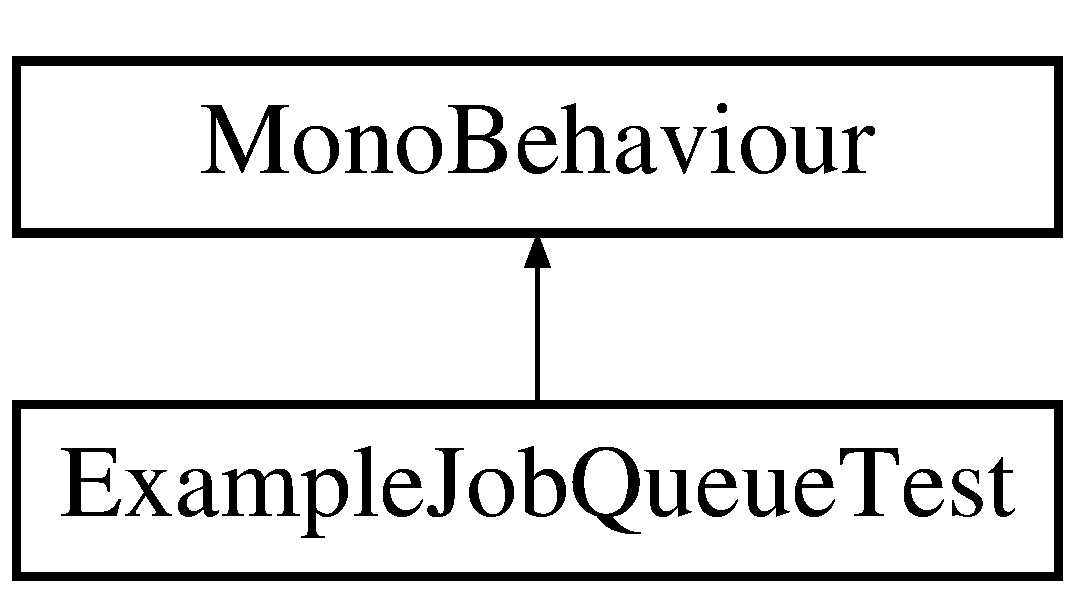
\includegraphics[height=2.000000cm]{class_example_job_queue_test}
\end{center}
\end{figure}
\subsection*{Public Member Functions}
\begin{DoxyCompactItemize}
\item 
I\+Enumerator \hyperlink{class_example_job_queue_test_a45a4cc204d6396b39b6ff3844c4dbc2f}{Simple\+Global\+Queue\+Test} ()
\begin{DoxyCompactList}\small\item\em Creates a list of jobs, adds them to the global queue and starts global queue. The global queue can be accessed from any script. \end{DoxyCompactList}\item 
I\+Enumerator \hyperlink{class_example_job_queue_test_a65d6aaf0f94ba848ce1be82a6d90e780}{Simple\+Local\+Queue\+Test} ()
\begin{DoxyCompactList}\small\item\em Creates a list of jobs, adds them to a newly created local queue and starts the queue. \end{DoxyCompactList}\item 
I\+Enumerator \hyperlink{class_example_job_queue_test_abe5f18a717e6699715d829f8fe797da5}{Local\+Queue\+Delayed\+Start\+Test} ()
\begin{DoxyCompactList}\small\item\em Creates and starts a queue after a delay of two seconds. \end{DoxyCompactList}\item 
I\+Enumerator \hyperlink{class_example_job_queue_test_a1463e2c77a6e293cb5d1a596a970d405}{Local\+Queue\+Delayed\+Pause\+And\+Resume\+Test} ()
\begin{DoxyCompactList}\small\item\em Creates a local queue, starts queue, pauses queue after 1 seconds, and lastly resumes queue after 3 seconds. \end{DoxyCompactList}\item 
I\+Enumerator \hyperlink{class_example_job_queue_test_ac09ae706637551c37837a36d951fbac6}{Queue\+Event\+Test} ()
\begin{DoxyCompactList}\small\item\em Subscribes to the global queue \char`\"{}queue\+Started\char`\"{}, \char`\"{}job\+Processed\char`\"{}, and \char`\"{}queue\+Complete\char`\"{} events. \end{DoxyCompactList}\item 
I\+Enumerator \hyperlink{class_example_job_queue_test_a56d063006d12236d417219ae1711706b}{Delayed\+Kill\+Current\+Test} ()
\begin{DoxyCompactList}\small\item\em Creates a local queue and sets the current job in the queue to be killed after three seconds. This kills the currently running job but the queue still executes. \end{DoxyCompactList}\item 
I\+Enumerator \hyperlink{class_example_job_queue_test_a3c5d23ccdb5c3edfd54ca39c4f93a22e}{Delayed\+Kill\+All\+Test} ()
\begin{DoxyCompactList}\small\item\em Creates a local queue and sets all jobs in the queue to be killed after one second. This kills all jobs and clears the queue. \end{DoxyCompactList}\item 
I\+Enumerator \hyperlink{class_example_job_queue_test_a628f7061c7818786b52a6b9371a1af6c}{Add\+Local\+Queue\+To\+Global\+Queue\+Test} ()
\begin{DoxyCompactList}\small\item\em Creates a local queue and then adds it to the glocal queue. The event subscriptions are also added to the global queue. \end{DoxyCompactList}\item 
I\+Enumerator \hyperlink{class_example_job_queue_test_a1ffd555683806c216251f462bb69cb40}{Add\+Repeating\+Job\+To\+Queue\+Test} ()
\begin{DoxyCompactList}\small\item\em Adds a repeating job to a queue. Queue will not progress if a repeating job is added until that job is manually killed or has reached its set number of times to repeat. \end{DoxyCompactList}\item 
I\+Enumerator \hyperlink{class_example_job_queue_test_a037cbad8b6d50077e844cb28e9412741}{Set\+Number\+Repeating\+Queue\+Test} ()
\begin{DoxyCompactList}\small\item\em Creates a new local queue, adds a number of test jobs and sets the queue to repeat two times. \end{DoxyCompactList}\item 
I\+Enumerator \hyperlink{class_example_job_queue_test_a3b7bf466ad7ad9b4039402a8fab519cf}{Timed\+Repeating\+Queue\+Test} ()
\begin{DoxyCompactList}\small\item\em Creates a new local queue, sets it to repeat and then stop repeating after 1 seconds. \end{DoxyCompactList}\item 
I\+Enumerator \hyperlink{class_example_job_queue_test_aee4d70589eda67ae5237f27c3398f19f}{Cloned\+Repeating\+Queue\+Test} ()
\begin{DoxyCompactList}\small\item\em Creates a local queue and sets it to repeat twice. The queue is then cloned and started. The new cloned queue will contain the original queues repeat status and event subscriptions. \end{DoxyCompactList}\item 
I\+Enumerator \hyperlink{class_example_job_queue_test_ac1f5d324d824d30fb115a012c97a7f68}{Multiple\+Cloned\+Queue\+Test} ()
\begin{DoxyCompactList}\small\item\em Creates a local queue and clones the queue twice. Both of the cloned queues are then started. \end{DoxyCompactList}\end{DoxyCompactItemize}


\subsection{Detailed Description}
Includes a number of methods to test the functionality of the \hyperlink{class_c_m___job_queue}{C\+M\+\_\+\+Job\+Queue} class. Each method showcases a particular functionality of the \hyperlink{class_c_m___job_queue}{C\+M\+\_\+\+Job\+Queue} that you can implement in your own projects. Each method returns an ienumerator so that it can added to a seperate job queue to be run in sequence for test purposes. 



\subsection{Member Function Documentation}
\hypertarget{class_example_job_queue_test_a628f7061c7818786b52a6b9371a1af6c}{}\index{Example\+Job\+Queue\+Test@{Example\+Job\+Queue\+Test}!Add\+Local\+Queue\+To\+Global\+Queue\+Test@{Add\+Local\+Queue\+To\+Global\+Queue\+Test}}
\index{Add\+Local\+Queue\+To\+Global\+Queue\+Test@{Add\+Local\+Queue\+To\+Global\+Queue\+Test}!Example\+Job\+Queue\+Test@{Example\+Job\+Queue\+Test}}
\subsubsection[{Add\+Local\+Queue\+To\+Global\+Queue\+Test()}]{\setlength{\rightskip}{0pt plus 5cm}I\+Enumerator Example\+Job\+Queue\+Test.\+Add\+Local\+Queue\+To\+Global\+Queue\+Test (
\begin{DoxyParamCaption}
{}
\end{DoxyParamCaption}
)}\label{class_example_job_queue_test_a628f7061c7818786b52a6b9371a1af6c}


Creates a local queue and then adds it to the glocal queue. The event subscriptions are also added to the global queue. 

\hypertarget{class_example_job_queue_test_a1ffd555683806c216251f462bb69cb40}{}\index{Example\+Job\+Queue\+Test@{Example\+Job\+Queue\+Test}!Add\+Repeating\+Job\+To\+Queue\+Test@{Add\+Repeating\+Job\+To\+Queue\+Test}}
\index{Add\+Repeating\+Job\+To\+Queue\+Test@{Add\+Repeating\+Job\+To\+Queue\+Test}!Example\+Job\+Queue\+Test@{Example\+Job\+Queue\+Test}}
\subsubsection[{Add\+Repeating\+Job\+To\+Queue\+Test()}]{\setlength{\rightskip}{0pt plus 5cm}I\+Enumerator Example\+Job\+Queue\+Test.\+Add\+Repeating\+Job\+To\+Queue\+Test (
\begin{DoxyParamCaption}
{}
\end{DoxyParamCaption}
)}\label{class_example_job_queue_test_a1ffd555683806c216251f462bb69cb40}


Adds a repeating job to a queue. Queue will not progress if a repeating job is added until that job is manually killed or has reached its set number of times to repeat. 

\hypertarget{class_example_job_queue_test_aee4d70589eda67ae5237f27c3398f19f}{}\index{Example\+Job\+Queue\+Test@{Example\+Job\+Queue\+Test}!Cloned\+Repeating\+Queue\+Test@{Cloned\+Repeating\+Queue\+Test}}
\index{Cloned\+Repeating\+Queue\+Test@{Cloned\+Repeating\+Queue\+Test}!Example\+Job\+Queue\+Test@{Example\+Job\+Queue\+Test}}
\subsubsection[{Cloned\+Repeating\+Queue\+Test()}]{\setlength{\rightskip}{0pt plus 5cm}I\+Enumerator Example\+Job\+Queue\+Test.\+Cloned\+Repeating\+Queue\+Test (
\begin{DoxyParamCaption}
{}
\end{DoxyParamCaption}
)}\label{class_example_job_queue_test_aee4d70589eda67ae5237f27c3398f19f}


Creates a local queue and sets it to repeat twice. The queue is then cloned and started. The new cloned queue will contain the original queues repeat status and event subscriptions. 

\hypertarget{class_example_job_queue_test_a3c5d23ccdb5c3edfd54ca39c4f93a22e}{}\index{Example\+Job\+Queue\+Test@{Example\+Job\+Queue\+Test}!Delayed\+Kill\+All\+Test@{Delayed\+Kill\+All\+Test}}
\index{Delayed\+Kill\+All\+Test@{Delayed\+Kill\+All\+Test}!Example\+Job\+Queue\+Test@{Example\+Job\+Queue\+Test}}
\subsubsection[{Delayed\+Kill\+All\+Test()}]{\setlength{\rightskip}{0pt plus 5cm}I\+Enumerator Example\+Job\+Queue\+Test.\+Delayed\+Kill\+All\+Test (
\begin{DoxyParamCaption}
{}
\end{DoxyParamCaption}
)}\label{class_example_job_queue_test_a3c5d23ccdb5c3edfd54ca39c4f93a22e}


Creates a local queue and sets all jobs in the queue to be killed after one second. This kills all jobs and clears the queue. 

\hypertarget{class_example_job_queue_test_a56d063006d12236d417219ae1711706b}{}\index{Example\+Job\+Queue\+Test@{Example\+Job\+Queue\+Test}!Delayed\+Kill\+Current\+Test@{Delayed\+Kill\+Current\+Test}}
\index{Delayed\+Kill\+Current\+Test@{Delayed\+Kill\+Current\+Test}!Example\+Job\+Queue\+Test@{Example\+Job\+Queue\+Test}}
\subsubsection[{Delayed\+Kill\+Current\+Test()}]{\setlength{\rightskip}{0pt plus 5cm}I\+Enumerator Example\+Job\+Queue\+Test.\+Delayed\+Kill\+Current\+Test (
\begin{DoxyParamCaption}
{}
\end{DoxyParamCaption}
)}\label{class_example_job_queue_test_a56d063006d12236d417219ae1711706b}


Creates a local queue and sets the current job in the queue to be killed after three seconds. This kills the currently running job but the queue still executes. 

\hypertarget{class_example_job_queue_test_a1463e2c77a6e293cb5d1a596a970d405}{}\index{Example\+Job\+Queue\+Test@{Example\+Job\+Queue\+Test}!Local\+Queue\+Delayed\+Pause\+And\+Resume\+Test@{Local\+Queue\+Delayed\+Pause\+And\+Resume\+Test}}
\index{Local\+Queue\+Delayed\+Pause\+And\+Resume\+Test@{Local\+Queue\+Delayed\+Pause\+And\+Resume\+Test}!Example\+Job\+Queue\+Test@{Example\+Job\+Queue\+Test}}
\subsubsection[{Local\+Queue\+Delayed\+Pause\+And\+Resume\+Test()}]{\setlength{\rightskip}{0pt plus 5cm}I\+Enumerator Example\+Job\+Queue\+Test.\+Local\+Queue\+Delayed\+Pause\+And\+Resume\+Test (
\begin{DoxyParamCaption}
{}
\end{DoxyParamCaption}
)}\label{class_example_job_queue_test_a1463e2c77a6e293cb5d1a596a970d405}


Creates a local queue, starts queue, pauses queue after 1 seconds, and lastly resumes queue after 3 seconds. 

\hypertarget{class_example_job_queue_test_abe5f18a717e6699715d829f8fe797da5}{}\index{Example\+Job\+Queue\+Test@{Example\+Job\+Queue\+Test}!Local\+Queue\+Delayed\+Start\+Test@{Local\+Queue\+Delayed\+Start\+Test}}
\index{Local\+Queue\+Delayed\+Start\+Test@{Local\+Queue\+Delayed\+Start\+Test}!Example\+Job\+Queue\+Test@{Example\+Job\+Queue\+Test}}
\subsubsection[{Local\+Queue\+Delayed\+Start\+Test()}]{\setlength{\rightskip}{0pt plus 5cm}I\+Enumerator Example\+Job\+Queue\+Test.\+Local\+Queue\+Delayed\+Start\+Test (
\begin{DoxyParamCaption}
{}
\end{DoxyParamCaption}
)}\label{class_example_job_queue_test_abe5f18a717e6699715d829f8fe797da5}


Creates and starts a queue after a delay of two seconds. 

\hypertarget{class_example_job_queue_test_ac1f5d324d824d30fb115a012c97a7f68}{}\index{Example\+Job\+Queue\+Test@{Example\+Job\+Queue\+Test}!Multiple\+Cloned\+Queue\+Test@{Multiple\+Cloned\+Queue\+Test}}
\index{Multiple\+Cloned\+Queue\+Test@{Multiple\+Cloned\+Queue\+Test}!Example\+Job\+Queue\+Test@{Example\+Job\+Queue\+Test}}
\subsubsection[{Multiple\+Cloned\+Queue\+Test()}]{\setlength{\rightskip}{0pt plus 5cm}I\+Enumerator Example\+Job\+Queue\+Test.\+Multiple\+Cloned\+Queue\+Test (
\begin{DoxyParamCaption}
{}
\end{DoxyParamCaption}
)}\label{class_example_job_queue_test_ac1f5d324d824d30fb115a012c97a7f68}


Creates a local queue and clones the queue twice. Both of the cloned queues are then started. 

\hypertarget{class_example_job_queue_test_ac09ae706637551c37837a36d951fbac6}{}\index{Example\+Job\+Queue\+Test@{Example\+Job\+Queue\+Test}!Queue\+Event\+Test@{Queue\+Event\+Test}}
\index{Queue\+Event\+Test@{Queue\+Event\+Test}!Example\+Job\+Queue\+Test@{Example\+Job\+Queue\+Test}}
\subsubsection[{Queue\+Event\+Test()}]{\setlength{\rightskip}{0pt plus 5cm}I\+Enumerator Example\+Job\+Queue\+Test.\+Queue\+Event\+Test (
\begin{DoxyParamCaption}
{}
\end{DoxyParamCaption}
)}\label{class_example_job_queue_test_ac09ae706637551c37837a36d951fbac6}


Subscribes to the global queue \char`\"{}queue\+Started\char`\"{}, \char`\"{}job\+Processed\char`\"{}, and \char`\"{}queue\+Complete\char`\"{} events. 

\hypertarget{class_example_job_queue_test_a037cbad8b6d50077e844cb28e9412741}{}\index{Example\+Job\+Queue\+Test@{Example\+Job\+Queue\+Test}!Set\+Number\+Repeating\+Queue\+Test@{Set\+Number\+Repeating\+Queue\+Test}}
\index{Set\+Number\+Repeating\+Queue\+Test@{Set\+Number\+Repeating\+Queue\+Test}!Example\+Job\+Queue\+Test@{Example\+Job\+Queue\+Test}}
\subsubsection[{Set\+Number\+Repeating\+Queue\+Test()}]{\setlength{\rightskip}{0pt plus 5cm}I\+Enumerator Example\+Job\+Queue\+Test.\+Set\+Number\+Repeating\+Queue\+Test (
\begin{DoxyParamCaption}
{}
\end{DoxyParamCaption}
)}\label{class_example_job_queue_test_a037cbad8b6d50077e844cb28e9412741}


Creates a new local queue, adds a number of test jobs and sets the queue to repeat two times. 

\hypertarget{class_example_job_queue_test_a45a4cc204d6396b39b6ff3844c4dbc2f}{}\index{Example\+Job\+Queue\+Test@{Example\+Job\+Queue\+Test}!Simple\+Global\+Queue\+Test@{Simple\+Global\+Queue\+Test}}
\index{Simple\+Global\+Queue\+Test@{Simple\+Global\+Queue\+Test}!Example\+Job\+Queue\+Test@{Example\+Job\+Queue\+Test}}
\subsubsection[{Simple\+Global\+Queue\+Test()}]{\setlength{\rightskip}{0pt plus 5cm}I\+Enumerator Example\+Job\+Queue\+Test.\+Simple\+Global\+Queue\+Test (
\begin{DoxyParamCaption}
{}
\end{DoxyParamCaption}
)}\label{class_example_job_queue_test_a45a4cc204d6396b39b6ff3844c4dbc2f}


Creates a list of jobs, adds them to the global queue and starts global queue. The global queue can be accessed from any script. 

\hypertarget{class_example_job_queue_test_a65d6aaf0f94ba848ce1be82a6d90e780}{}\index{Example\+Job\+Queue\+Test@{Example\+Job\+Queue\+Test}!Simple\+Local\+Queue\+Test@{Simple\+Local\+Queue\+Test}}
\index{Simple\+Local\+Queue\+Test@{Simple\+Local\+Queue\+Test}!Example\+Job\+Queue\+Test@{Example\+Job\+Queue\+Test}}
\subsubsection[{Simple\+Local\+Queue\+Test()}]{\setlength{\rightskip}{0pt plus 5cm}I\+Enumerator Example\+Job\+Queue\+Test.\+Simple\+Local\+Queue\+Test (
\begin{DoxyParamCaption}
{}
\end{DoxyParamCaption}
)}\label{class_example_job_queue_test_a65d6aaf0f94ba848ce1be82a6d90e780}


Creates a list of jobs, adds them to a newly created local queue and starts the queue. 

\hypertarget{class_example_job_queue_test_a3b7bf466ad7ad9b4039402a8fab519cf}{}\index{Example\+Job\+Queue\+Test@{Example\+Job\+Queue\+Test}!Timed\+Repeating\+Queue\+Test@{Timed\+Repeating\+Queue\+Test}}
\index{Timed\+Repeating\+Queue\+Test@{Timed\+Repeating\+Queue\+Test}!Example\+Job\+Queue\+Test@{Example\+Job\+Queue\+Test}}
\subsubsection[{Timed\+Repeating\+Queue\+Test()}]{\setlength{\rightskip}{0pt plus 5cm}I\+Enumerator Example\+Job\+Queue\+Test.\+Timed\+Repeating\+Queue\+Test (
\begin{DoxyParamCaption}
{}
\end{DoxyParamCaption}
)}\label{class_example_job_queue_test_a3b7bf466ad7ad9b4039402a8fab519cf}


Creates a new local queue, sets it to repeat and then stop repeating after 1 seconds. 



The documentation for this class was generated from the following file\+:\begin{DoxyCompactItemize}
\item 
Example\+Job\+Queue\+Test.\+cs\end{DoxyCompactItemize}

\hypertarget{class_example_job_test}{}\section{Example\+Job\+Test Class Reference}
\label{class_example_job_test}\index{Example\+Job\+Test@{Example\+Job\+Test}}


Includes a number of methods to test the functionality of the \hyperlink{class_c_m___job}{C\+M\+\_\+\+Job} class. Each method showcases a particular functionality of the \hyperlink{class_c_m___job}{C\+M\+\_\+\+Job} class that you can implement in your own projects. Each method returns an ienumerator so that it can added to a job queue to be run in sequence for test purposes.  


Inheritance diagram for Example\+Job\+Test\+:\begin{figure}[H]
\begin{center}
\leavevmode
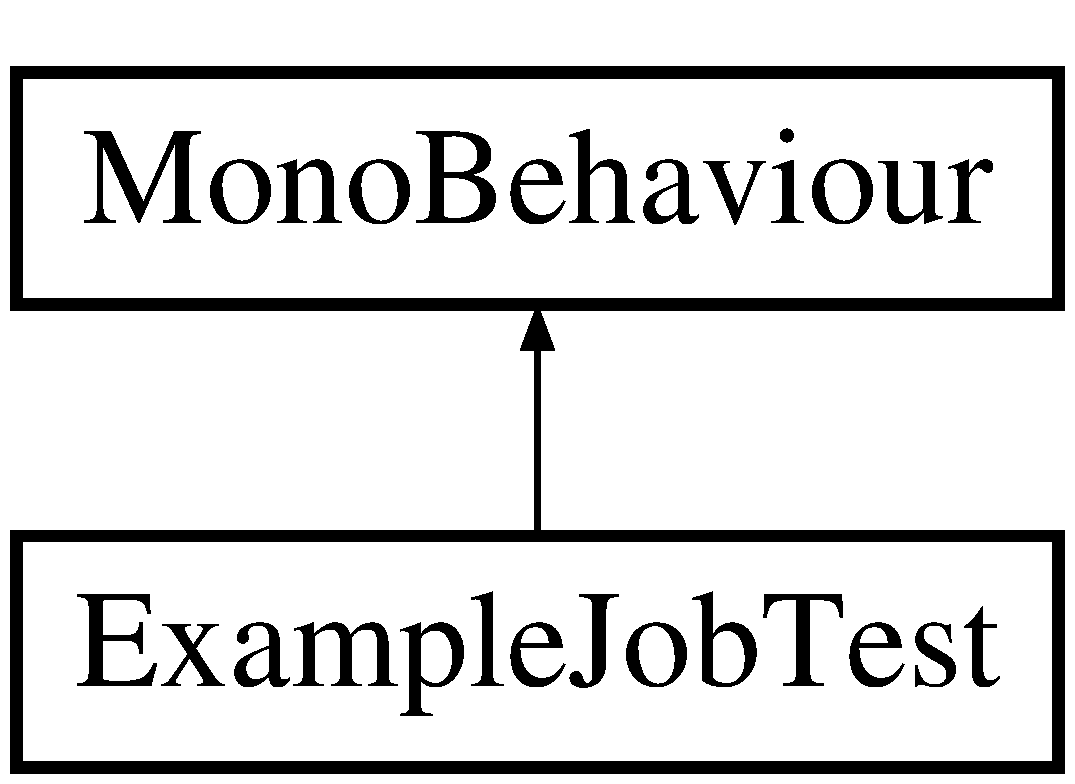
\includegraphics[height=2.000000cm]{class_example_job_test}
\end{center}
\end{figure}
\subsection*{Public Member Functions}
\begin{DoxyCompactItemize}
\item 
I\+Enumerator \hyperlink{class_example_job_test_ab235738389e731b6e1c1a0936bfb6585}{Simple\+Job\+Test} ()
\begin{DoxyCompactList}\small\item\em Creates and starts a job. \end{DoxyCompactList}\item 
I\+Enumerator \hyperlink{class_example_job_test_a1bf38c8133ef7854e4b3ef89103888df}{Job\+Test\+With\+Delayed\+Start} ()
\begin{DoxyCompactList}\small\item\em Creates and starts a job after a delay. \end{DoxyCompactList}\item 
I\+Enumerator \hyperlink{class_example_job_test_ac390bb8191f6ba7b6df2deb646c7c7de}{Job\+Test\+With\+Delayed\+Pause} ()
\begin{DoxyCompactList}\small\item\em Creates coroutine job, starts job immediately and then pauses coroutine after 4 seconds. This paused job is then stored and can be resumed/killed from any class that has a reference to that job. \end{DoxyCompactList}\item 
I\+Enumerator \hyperlink{class_example_job_test_af80fb4b62309ca6833878c49b82df703}{Job\+Test\+With\+Delayed\+Resume} ()
\begin{DoxyCompactList}\small\item\em Creates new job, pauses after 1 second, and resumes after 3 seconds. \end{DoxyCompactList}\item 
I\+Enumerator \hyperlink{class_example_job_test_a95678534abfb975339db76044a92b28d}{Job\+Test\+With\+Delayed\+Kill} ()
\begin{DoxyCompactList}\small\item\em Creates coroutine job, starts job immediately and then sets the job to be killed after 4 seconds. \end{DoxyCompactList}\item 
I\+Enumerator \hyperlink{class_example_job_test_a5c211a493fa17b33b35ba64214d1bb09}{Job\+Test\+With\+Start\+And\+End\+Events} ()
\begin{DoxyCompactList}\small\item\em Creates new job, subscribes to the job start and end events and then starts job to be run immediately. \end{DoxyCompactList}\item 
I\+Enumerator \hyperlink{class_example_job_test_a95dc6aea129056f6565484c7efd6ab03}{Child\+Job\+Test} ()
\begin{DoxyCompactList}\small\item\em Child job test. Creates new job, adds two children (parent will not complete until children have finished processing) and starts the job. \end{DoxyCompactList}\item 
I\+Enumerator \hyperlink{class_example_job_test_a7a5819f751f3ba68941dd5530bf7a365}{Single\+Clone\+Job\+Test} ()
\begin{DoxyCompactList}\small\item\em Creates a new job, clones job, and then runs clone. \end{DoxyCompactList}\item 
I\+Enumerator \hyperlink{class_example_job_test_a707273ae104f9aac979fa8d697e306b5}{Multiple\+Clone\+Job\+Test} ()
\begin{DoxyCompactList}\small\item\em Creates a new job, clones five copies of the original job, and then starts a random clone. \end{DoxyCompactList}\item 
I\+Enumerator \hyperlink{class_example_job_test_a8941dbc9a2ba2c401785414a669b6331}{Infinitely\+Repeatable\+Job\+Test} ()
\begin{DoxyCompactList}\small\item\em Creates and starts a job that will repeat for 3 seconds. The job complete event is subscribed to, this is used to display how many times the job will be repeated. \end{DoxyCompactList}\item 
I\+Enumerator \hyperlink{class_example_job_test_a11f7ec3104852950a7f35208b75671e5}{Multiple\+Repeatable\+Job\+Test} ()
\begin{DoxyCompactList}\small\item\em Creates and starts a job that will repeat three times. The job complete event is subscribed to, this is used to display how many times the job will be repeated. \end{DoxyCompactList}\item 
I\+Enumerator \hyperlink{class_example_job_test_a4d476fb823d8c82dfe1fe17f37d4fdf7}{Mutltiple\+Repeatable\+Job\+Test\+With\+Child} ()
\begin{DoxyCompactList}\small\item\em Creates and starts a job that will repeat three times. Adds a child job that will also repeat three times. The job complete event and child job complete events are subscribed to, this is used to display how many times the job will be repeated. \end{DoxyCompactList}\end{DoxyCompactItemize}


\subsection{Detailed Description}
Includes a number of methods to test the functionality of the \hyperlink{class_c_m___job}{C\+M\+\_\+\+Job} class. Each method showcases a particular functionality of the \hyperlink{class_c_m___job}{C\+M\+\_\+\+Job} class that you can implement in your own projects. Each method returns an ienumerator so that it can added to a job queue to be run in sequence for test purposes. 



\subsection{Member Function Documentation}
\hypertarget{class_example_job_test_a95dc6aea129056f6565484c7efd6ab03}{}\index{Example\+Job\+Test@{Example\+Job\+Test}!Child\+Job\+Test@{Child\+Job\+Test}}
\index{Child\+Job\+Test@{Child\+Job\+Test}!Example\+Job\+Test@{Example\+Job\+Test}}
\subsubsection[{Child\+Job\+Test()}]{\setlength{\rightskip}{0pt plus 5cm}I\+Enumerator Example\+Job\+Test.\+Child\+Job\+Test (
\begin{DoxyParamCaption}
{}
\end{DoxyParamCaption}
)}\label{class_example_job_test_a95dc6aea129056f6565484c7efd6ab03}


Child job test. Creates new job, adds two children (parent will not complete until children have finished processing) and starts the job. 

\hypertarget{class_example_job_test_a8941dbc9a2ba2c401785414a669b6331}{}\index{Example\+Job\+Test@{Example\+Job\+Test}!Infinitely\+Repeatable\+Job\+Test@{Infinitely\+Repeatable\+Job\+Test}}
\index{Infinitely\+Repeatable\+Job\+Test@{Infinitely\+Repeatable\+Job\+Test}!Example\+Job\+Test@{Example\+Job\+Test}}
\subsubsection[{Infinitely\+Repeatable\+Job\+Test()}]{\setlength{\rightskip}{0pt plus 5cm}I\+Enumerator Example\+Job\+Test.\+Infinitely\+Repeatable\+Job\+Test (
\begin{DoxyParamCaption}
{}
\end{DoxyParamCaption}
)}\label{class_example_job_test_a8941dbc9a2ba2c401785414a669b6331}


Creates and starts a job that will repeat for 3 seconds. The job complete event is subscribed to, this is used to display how many times the job will be repeated. 

\hypertarget{class_example_job_test_a95678534abfb975339db76044a92b28d}{}\index{Example\+Job\+Test@{Example\+Job\+Test}!Job\+Test\+With\+Delayed\+Kill@{Job\+Test\+With\+Delayed\+Kill}}
\index{Job\+Test\+With\+Delayed\+Kill@{Job\+Test\+With\+Delayed\+Kill}!Example\+Job\+Test@{Example\+Job\+Test}}
\subsubsection[{Job\+Test\+With\+Delayed\+Kill()}]{\setlength{\rightskip}{0pt plus 5cm}I\+Enumerator Example\+Job\+Test.\+Job\+Test\+With\+Delayed\+Kill (
\begin{DoxyParamCaption}
{}
\end{DoxyParamCaption}
)}\label{class_example_job_test_a95678534abfb975339db76044a92b28d}


Creates coroutine job, starts job immediately and then sets the job to be killed after 4 seconds. 

\hypertarget{class_example_job_test_ac390bb8191f6ba7b6df2deb646c7c7de}{}\index{Example\+Job\+Test@{Example\+Job\+Test}!Job\+Test\+With\+Delayed\+Pause@{Job\+Test\+With\+Delayed\+Pause}}
\index{Job\+Test\+With\+Delayed\+Pause@{Job\+Test\+With\+Delayed\+Pause}!Example\+Job\+Test@{Example\+Job\+Test}}
\subsubsection[{Job\+Test\+With\+Delayed\+Pause()}]{\setlength{\rightskip}{0pt plus 5cm}I\+Enumerator Example\+Job\+Test.\+Job\+Test\+With\+Delayed\+Pause (
\begin{DoxyParamCaption}
{}
\end{DoxyParamCaption}
)}\label{class_example_job_test_ac390bb8191f6ba7b6df2deb646c7c7de}


Creates coroutine job, starts job immediately and then pauses coroutine after 4 seconds. This paused job is then stored and can be resumed/killed from any class that has a reference to that job. 

\hypertarget{class_example_job_test_af80fb4b62309ca6833878c49b82df703}{}\index{Example\+Job\+Test@{Example\+Job\+Test}!Job\+Test\+With\+Delayed\+Resume@{Job\+Test\+With\+Delayed\+Resume}}
\index{Job\+Test\+With\+Delayed\+Resume@{Job\+Test\+With\+Delayed\+Resume}!Example\+Job\+Test@{Example\+Job\+Test}}
\subsubsection[{Job\+Test\+With\+Delayed\+Resume()}]{\setlength{\rightskip}{0pt plus 5cm}I\+Enumerator Example\+Job\+Test.\+Job\+Test\+With\+Delayed\+Resume (
\begin{DoxyParamCaption}
{}
\end{DoxyParamCaption}
)}\label{class_example_job_test_af80fb4b62309ca6833878c49b82df703}


Creates new job, pauses after 1 second, and resumes after 3 seconds. 

\hypertarget{class_example_job_test_a1bf38c8133ef7854e4b3ef89103888df}{}\index{Example\+Job\+Test@{Example\+Job\+Test}!Job\+Test\+With\+Delayed\+Start@{Job\+Test\+With\+Delayed\+Start}}
\index{Job\+Test\+With\+Delayed\+Start@{Job\+Test\+With\+Delayed\+Start}!Example\+Job\+Test@{Example\+Job\+Test}}
\subsubsection[{Job\+Test\+With\+Delayed\+Start()}]{\setlength{\rightskip}{0pt plus 5cm}I\+Enumerator Example\+Job\+Test.\+Job\+Test\+With\+Delayed\+Start (
\begin{DoxyParamCaption}
{}
\end{DoxyParamCaption}
)}\label{class_example_job_test_a1bf38c8133ef7854e4b3ef89103888df}


Creates and starts a job after a delay. 

\hypertarget{class_example_job_test_a5c211a493fa17b33b35ba64214d1bb09}{}\index{Example\+Job\+Test@{Example\+Job\+Test}!Job\+Test\+With\+Start\+And\+End\+Events@{Job\+Test\+With\+Start\+And\+End\+Events}}
\index{Job\+Test\+With\+Start\+And\+End\+Events@{Job\+Test\+With\+Start\+And\+End\+Events}!Example\+Job\+Test@{Example\+Job\+Test}}
\subsubsection[{Job\+Test\+With\+Start\+And\+End\+Events()}]{\setlength{\rightskip}{0pt plus 5cm}I\+Enumerator Example\+Job\+Test.\+Job\+Test\+With\+Start\+And\+End\+Events (
\begin{DoxyParamCaption}
{}
\end{DoxyParamCaption}
)}\label{class_example_job_test_a5c211a493fa17b33b35ba64214d1bb09}


Creates new job, subscribes to the job start and end events and then starts job to be run immediately. 

\hypertarget{class_example_job_test_a707273ae104f9aac979fa8d697e306b5}{}\index{Example\+Job\+Test@{Example\+Job\+Test}!Multiple\+Clone\+Job\+Test@{Multiple\+Clone\+Job\+Test}}
\index{Multiple\+Clone\+Job\+Test@{Multiple\+Clone\+Job\+Test}!Example\+Job\+Test@{Example\+Job\+Test}}
\subsubsection[{Multiple\+Clone\+Job\+Test()}]{\setlength{\rightskip}{0pt plus 5cm}I\+Enumerator Example\+Job\+Test.\+Multiple\+Clone\+Job\+Test (
\begin{DoxyParamCaption}
{}
\end{DoxyParamCaption}
)}\label{class_example_job_test_a707273ae104f9aac979fa8d697e306b5}


Creates a new job, clones five copies of the original job, and then starts a random clone. 

\hypertarget{class_example_job_test_a11f7ec3104852950a7f35208b75671e5}{}\index{Example\+Job\+Test@{Example\+Job\+Test}!Multiple\+Repeatable\+Job\+Test@{Multiple\+Repeatable\+Job\+Test}}
\index{Multiple\+Repeatable\+Job\+Test@{Multiple\+Repeatable\+Job\+Test}!Example\+Job\+Test@{Example\+Job\+Test}}
\subsubsection[{Multiple\+Repeatable\+Job\+Test()}]{\setlength{\rightskip}{0pt plus 5cm}I\+Enumerator Example\+Job\+Test.\+Multiple\+Repeatable\+Job\+Test (
\begin{DoxyParamCaption}
{}
\end{DoxyParamCaption}
)}\label{class_example_job_test_a11f7ec3104852950a7f35208b75671e5}


Creates and starts a job that will repeat three times. The job complete event is subscribed to, this is used to display how many times the job will be repeated. 

\hypertarget{class_example_job_test_a4d476fb823d8c82dfe1fe17f37d4fdf7}{}\index{Example\+Job\+Test@{Example\+Job\+Test}!Mutltiple\+Repeatable\+Job\+Test\+With\+Child@{Mutltiple\+Repeatable\+Job\+Test\+With\+Child}}
\index{Mutltiple\+Repeatable\+Job\+Test\+With\+Child@{Mutltiple\+Repeatable\+Job\+Test\+With\+Child}!Example\+Job\+Test@{Example\+Job\+Test}}
\subsubsection[{Mutltiple\+Repeatable\+Job\+Test\+With\+Child()}]{\setlength{\rightskip}{0pt plus 5cm}I\+Enumerator Example\+Job\+Test.\+Mutltiple\+Repeatable\+Job\+Test\+With\+Child (
\begin{DoxyParamCaption}
{}
\end{DoxyParamCaption}
)}\label{class_example_job_test_a4d476fb823d8c82dfe1fe17f37d4fdf7}


Creates and starts a job that will repeat three times. Adds a child job that will also repeat three times. The job complete event and child job complete events are subscribed to, this is used to display how many times the job will be repeated. 

\hypertarget{class_example_job_test_ab235738389e731b6e1c1a0936bfb6585}{}\index{Example\+Job\+Test@{Example\+Job\+Test}!Simple\+Job\+Test@{Simple\+Job\+Test}}
\index{Simple\+Job\+Test@{Simple\+Job\+Test}!Example\+Job\+Test@{Example\+Job\+Test}}
\subsubsection[{Simple\+Job\+Test()}]{\setlength{\rightskip}{0pt plus 5cm}I\+Enumerator Example\+Job\+Test.\+Simple\+Job\+Test (
\begin{DoxyParamCaption}
{}
\end{DoxyParamCaption}
)}\label{class_example_job_test_ab235738389e731b6e1c1a0936bfb6585}


Creates and starts a job. 

\hypertarget{class_example_job_test_a7a5819f751f3ba68941dd5530bf7a365}{}\index{Example\+Job\+Test@{Example\+Job\+Test}!Single\+Clone\+Job\+Test@{Single\+Clone\+Job\+Test}}
\index{Single\+Clone\+Job\+Test@{Single\+Clone\+Job\+Test}!Example\+Job\+Test@{Example\+Job\+Test}}
\subsubsection[{Single\+Clone\+Job\+Test()}]{\setlength{\rightskip}{0pt plus 5cm}I\+Enumerator Example\+Job\+Test.\+Single\+Clone\+Job\+Test (
\begin{DoxyParamCaption}
{}
\end{DoxyParamCaption}
)}\label{class_example_job_test_a7a5819f751f3ba68941dd5530bf7a365}


Creates a new job, clones job, and then runs clone. 



The documentation for this class was generated from the following file\+:\begin{DoxyCompactItemize}
\item 
Example\+Job\+Test.\+cs\end{DoxyCompactItemize}

\hypertarget{class_example_timer}{}\section{Example\+Timer Class Reference}
\label{class_example_timer}\index{Example\+Timer@{Example\+Timer}}


Creates new coroutine job to update a text object with time since startup. Adds job to global job manager so that it can be paused and resumed as required.  


Inheritance diagram for Example\+Timer\+:\begin{figure}[H]
\begin{center}
\leavevmode
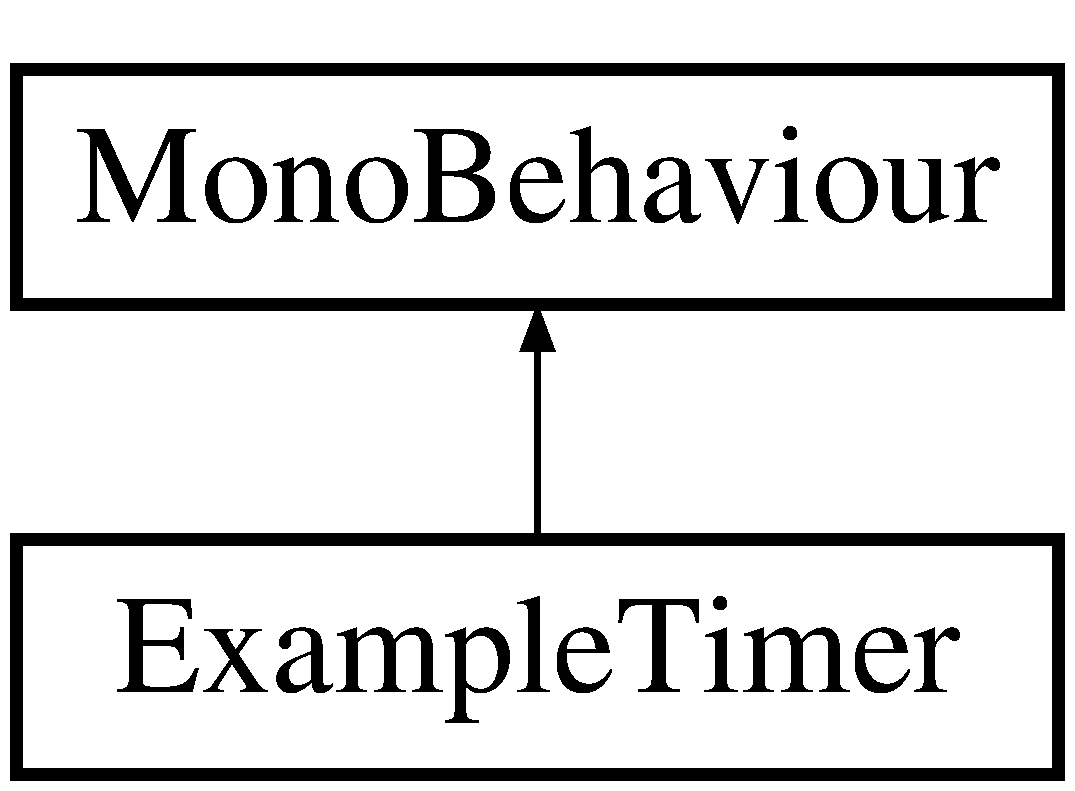
\includegraphics[height=2.000000cm]{class_example_timer}
\end{center}
\end{figure}


\subsection{Detailed Description}
Creates new coroutine job to update a text object with time since startup. Adds job to global job manager so that it can be paused and resumed as required. 



The documentation for this class was generated from the following file\+:\begin{DoxyCompactItemize}
\item 
Example\+Timer.\+cs\end{DoxyCompactItemize}

\hypertarget{class_example_t_imer_pause_resume}{}\section{Example\+T\+Imer\+Pause\+Resume Class Reference}
\label{class_example_t_imer_pause_resume}\index{Example\+T\+Imer\+Pause\+Resume@{Example\+T\+Imer\+Pause\+Resume}}


Pauses all jobs associated with the Job\+Manager when user clicks left mouse button and resumes all jobs with user clicks right mouse button.  


Inheritance diagram for Example\+T\+Imer\+Pause\+Resume\+:\begin{figure}[H]
\begin{center}
\leavevmode
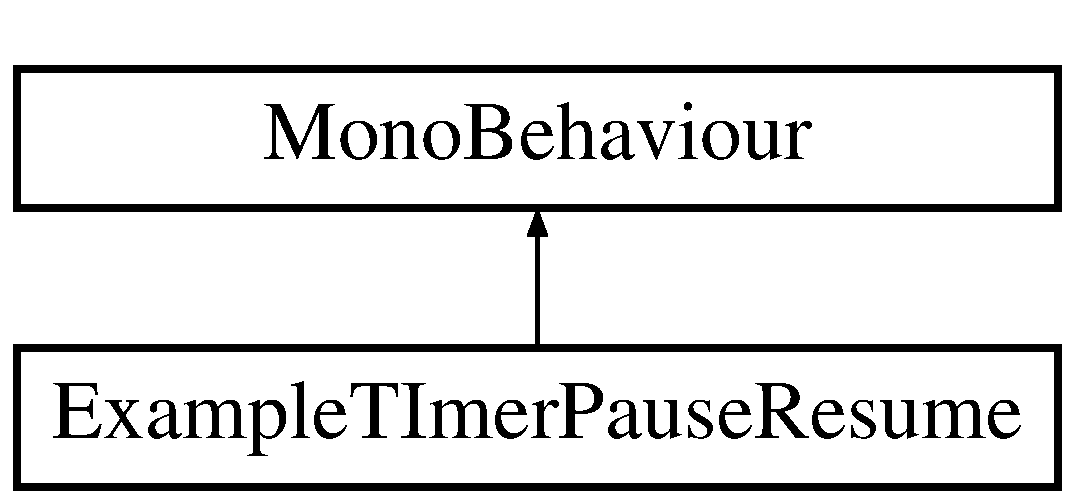
\includegraphics[height=2.000000cm]{class_example_t_imer_pause_resume}
\end{center}
\end{figure}


\subsection{Detailed Description}
Pauses all jobs associated with the Job\+Manager when user clicks left mouse button and resumes all jobs with user clicks right mouse button. 



The documentation for this class was generated from the following file\+:\begin{DoxyCompactItemize}
\item 
Example\+T\+Imer\+Pause\+Resume.\+cs\end{DoxyCompactItemize}

\hypertarget{interface_i_c_m___cloneable}{}\section{I\+C\+M\+\_\+\+Cloneable$<$ T $>$ Interface Template Reference}
\label{interface_i_c_m___cloneable}\index{I\+C\+M\+\_\+\+Cloneable$<$ T $>$@{I\+C\+M\+\_\+\+Cloneable$<$ T $>$}}


An interface for all classes used by the coroutine manager that can be cloned.  


\subsection*{Public Member Functions}
\begin{DoxyCompactItemize}
\item 
T \hyperlink{interface_i_c_m___cloneable_ae8b9fb9338e27c094a82d75a0c6c25ac}{Clone} ()
\begin{DoxyCompactList}\small\item\em Clone this instance. \end{DoxyCompactList}\item 
T\mbox{[}$\,$\mbox{]} \hyperlink{interface_i_c_m___cloneable_a2b520d18d778c682836ecc870155a5d8}{Clone} (int num\+Of\+Copies)
\begin{DoxyCompactList}\small\item\em Clone the specified num\+Of\+Copies. \end{DoxyCompactList}\end{DoxyCompactItemize}


\subsection{Detailed Description}
An interface for all classes used by the coroutine manager that can be cloned. 



\subsection{Member Function Documentation}
\hypertarget{interface_i_c_m___cloneable_ae8b9fb9338e27c094a82d75a0c6c25ac}{}\index{I\+C\+M\+\_\+\+Cloneable@{I\+C\+M\+\_\+\+Cloneable}!Clone@{Clone}}
\index{Clone@{Clone}!I\+C\+M\+\_\+\+Cloneable@{I\+C\+M\+\_\+\+Cloneable}}
\subsubsection[{Clone()}]{\setlength{\rightskip}{0pt plus 5cm}T {\bf I\+C\+M\+\_\+\+Cloneable}$<$ T $>$.Clone (
\begin{DoxyParamCaption}
{}
\end{DoxyParamCaption}
)}\label{interface_i_c_m___cloneable_ae8b9fb9338e27c094a82d75a0c6c25ac}


Clone this instance. 

\hypertarget{interface_i_c_m___cloneable_a2b520d18d778c682836ecc870155a5d8}{}\index{I\+C\+M\+\_\+\+Cloneable@{I\+C\+M\+\_\+\+Cloneable}!Clone@{Clone}}
\index{Clone@{Clone}!I\+C\+M\+\_\+\+Cloneable@{I\+C\+M\+\_\+\+Cloneable}}
\subsubsection[{Clone(int num\+Of\+Copies)}]{\setlength{\rightskip}{0pt plus 5cm}T \mbox{[}$\,$\mbox{]} {\bf I\+C\+M\+\_\+\+Cloneable}$<$ T $>$.Clone (
\begin{DoxyParamCaption}
\item[{int}]{num\+Of\+Copies}
\end{DoxyParamCaption}
)}\label{interface_i_c_m___cloneable_a2b520d18d778c682836ecc870155a5d8}


Clone the specified num\+Of\+Copies. 


\begin{DoxyParams}{Parameters}
{\em num\+Of\+Copies} & Number of copies.\\
\hline
\end{DoxyParams}


The documentation for this interface was generated from the following file\+:\begin{DoxyCompactItemize}
\item 
I\+C\+M\+\_\+\+Cloneable.\+cs\end{DoxyCompactItemize}

\hypertarget{class_c_m___logger_1_1_message}{}\section{C\+M\+\_\+\+Logger.\+Message Class Reference}
\label{class_c_m___logger_1_1_message}\index{C\+M\+\_\+\+Logger.\+Message@{C\+M\+\_\+\+Logger.\+Message}}


Encapsulates a message used by \hyperlink{class_c_m___logger}{C\+M\+\_\+\+Logger}.  


\subsection*{Public Member Functions}
\begin{DoxyCompactItemize}
\item 
\hyperlink{class_c_m___logger_1_1_message_af8da84fc7f2102870ce62695f3e2a38a}{Message} (object \hyperlink{class_c_m___logger_1_1_message_ad9921bbcd73048b60d9ba2c3b77286ae}{invoker}, object \hyperlink{class_c_m___logger_1_1_message_ac403c59f0f7f9452ad2cc3d7abf22844}{content})
\begin{DoxyCompactList}\small\item\em Initializes a new instance of the C\+M\+\_\+\+Logger+\+Message class. \end{DoxyCompactList}\item 
override string \hyperlink{class_c_m___logger_1_1_message_a011dbf54bd844f4400f30d9acacee254}{To\+String} ()
\begin{DoxyCompactList}\small\item\em Returns a System.\+String that represents the current C\+M\+\_\+\+Logger+\+Message. \end{DoxyCompactList}\end{DoxyCompactItemize}
\subsection*{Properties}
\begin{DoxyCompactItemize}
\item 
object \hyperlink{class_c_m___logger_1_1_message_ac403c59f0f7f9452ad2cc3d7abf22844}{content}\hspace{0.3cm}{\ttfamily  \mbox{[}get\mbox{]}}
\begin{DoxyCompactList}\small\item\em Gets the content of the message. \end{DoxyCompactList}\item 
object \hyperlink{class_c_m___logger_1_1_message_ad9921bbcd73048b60d9ba2c3b77286ae}{invoker}\hspace{0.3cm}{\ttfamily  \mbox{[}get\mbox{]}}
\begin{DoxyCompactList}\small\item\em Gets the invoker of the message. \end{DoxyCompactList}\end{DoxyCompactItemize}


\subsection{Detailed Description}
Encapsulates a message used by \hyperlink{class_c_m___logger}{C\+M\+\_\+\+Logger}. 



\subsection{Constructor \& Destructor Documentation}
\hypertarget{class_c_m___logger_1_1_message_af8da84fc7f2102870ce62695f3e2a38a}{}\index{C\+M\+\_\+\+Logger\+::\+Message@{C\+M\+\_\+\+Logger\+::\+Message}!Message@{Message}}
\index{Message@{Message}!C\+M\+\_\+\+Logger\+::\+Message@{C\+M\+\_\+\+Logger\+::\+Message}}
\subsubsection[{Message(object invoker, object content)}]{\setlength{\rightskip}{0pt plus 5cm}C\+M\+\_\+\+Logger.\+Message.\+Message (
\begin{DoxyParamCaption}
\item[{object}]{invoker, }
\item[{object}]{content}
\end{DoxyParamCaption}
)}\label{class_c_m___logger_1_1_message_af8da84fc7f2102870ce62695f3e2a38a}


Initializes a new instance of the C\+M\+\_\+\+Logger+\+Message class. 


\begin{DoxyParams}{Parameters}
{\em invoker} & Invoker.\\
\hline
{\em content} & Content.\\
\hline
\end{DoxyParams}


\subsection{Member Function Documentation}
\hypertarget{class_c_m___logger_1_1_message_a011dbf54bd844f4400f30d9acacee254}{}\index{C\+M\+\_\+\+Logger\+::\+Message@{C\+M\+\_\+\+Logger\+::\+Message}!To\+String@{To\+String}}
\index{To\+String@{To\+String}!C\+M\+\_\+\+Logger\+::\+Message@{C\+M\+\_\+\+Logger\+::\+Message}}
\subsubsection[{To\+String()}]{\setlength{\rightskip}{0pt plus 5cm}override string C\+M\+\_\+\+Logger.\+Message.\+To\+String (
\begin{DoxyParamCaption}
{}
\end{DoxyParamCaption}
)}\label{class_c_m___logger_1_1_message_a011dbf54bd844f4400f30d9acacee254}


Returns a System.\+String that represents the current C\+M\+\_\+\+Logger+\+Message. 

\begin{DoxyReturn}{Returns}
A System.\+String that represents the current C\+M\+\_\+\+Logger+\+Message.
\end{DoxyReturn}


\subsection{Property Documentation}
\hypertarget{class_c_m___logger_1_1_message_ac403c59f0f7f9452ad2cc3d7abf22844}{}\index{C\+M\+\_\+\+Logger\+::\+Message@{C\+M\+\_\+\+Logger\+::\+Message}!content@{content}}
\index{content@{content}!C\+M\+\_\+\+Logger\+::\+Message@{C\+M\+\_\+\+Logger\+::\+Message}}
\subsubsection[{content}]{\setlength{\rightskip}{0pt plus 5cm}object C\+M\+\_\+\+Logger.\+Message.\+content\hspace{0.3cm}{\ttfamily [get]}}\label{class_c_m___logger_1_1_message_ac403c59f0f7f9452ad2cc3d7abf22844}


Gets the content of the message. 

The content.\hypertarget{class_c_m___logger_1_1_message_ad9921bbcd73048b60d9ba2c3b77286ae}{}\index{C\+M\+\_\+\+Logger\+::\+Message@{C\+M\+\_\+\+Logger\+::\+Message}!invoker@{invoker}}
\index{invoker@{invoker}!C\+M\+\_\+\+Logger\+::\+Message@{C\+M\+\_\+\+Logger\+::\+Message}}
\subsubsection[{invoker}]{\setlength{\rightskip}{0pt plus 5cm}object C\+M\+\_\+\+Logger.\+Message.\+invoker\hspace{0.3cm}{\ttfamily [get]}}\label{class_c_m___logger_1_1_message_ad9921bbcd73048b60d9ba2c3b77286ae}


Gets the invoker of the message. 

The invoker.

The documentation for this class was generated from the following file\+:\begin{DoxyCompactItemize}
\item 
C\+M\+\_\+\+Logger.\+cs\end{DoxyCompactItemize}

%--- End generated contents ---

% Index
\backmatter
\newpage
\phantomsection
\clearemptydoublepage
\addcontentsline{toc}{chapter}{Index}
\printindex

\end{document}
